\documentclass[12pt]{article}
\usepackage[utf8]{inputenc}
\usepackage[letterpaper, margin=0.25in, headheight=10pt]{geometry}
\usepackage{amsmath}
\usepackage{amssymb}
\usepackage{graphicx}
\usepackage{pdflscape}

\newcommand\figWidth{7in}
\newcommand\figWidthLarge{7in}

\begin{document}

\begin{figure}
    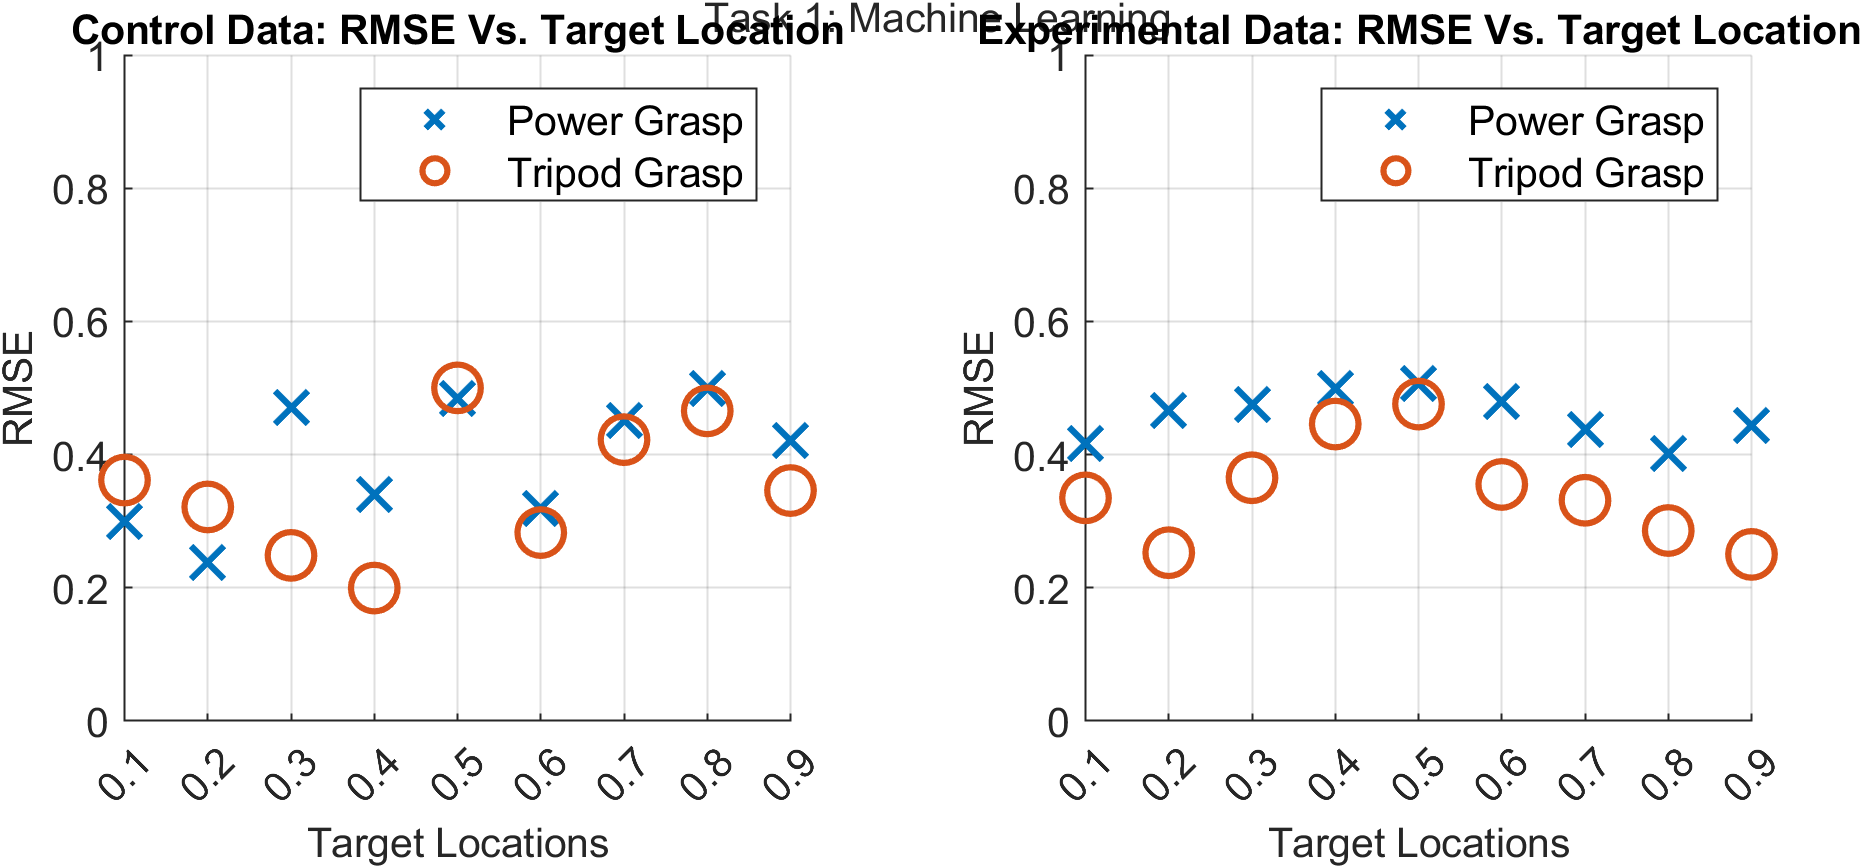
\includegraphics[width = \figWidth]{t1-rmse-reg.png}
\end{figure}
\newpage
\clearpage
\begin{figure}
    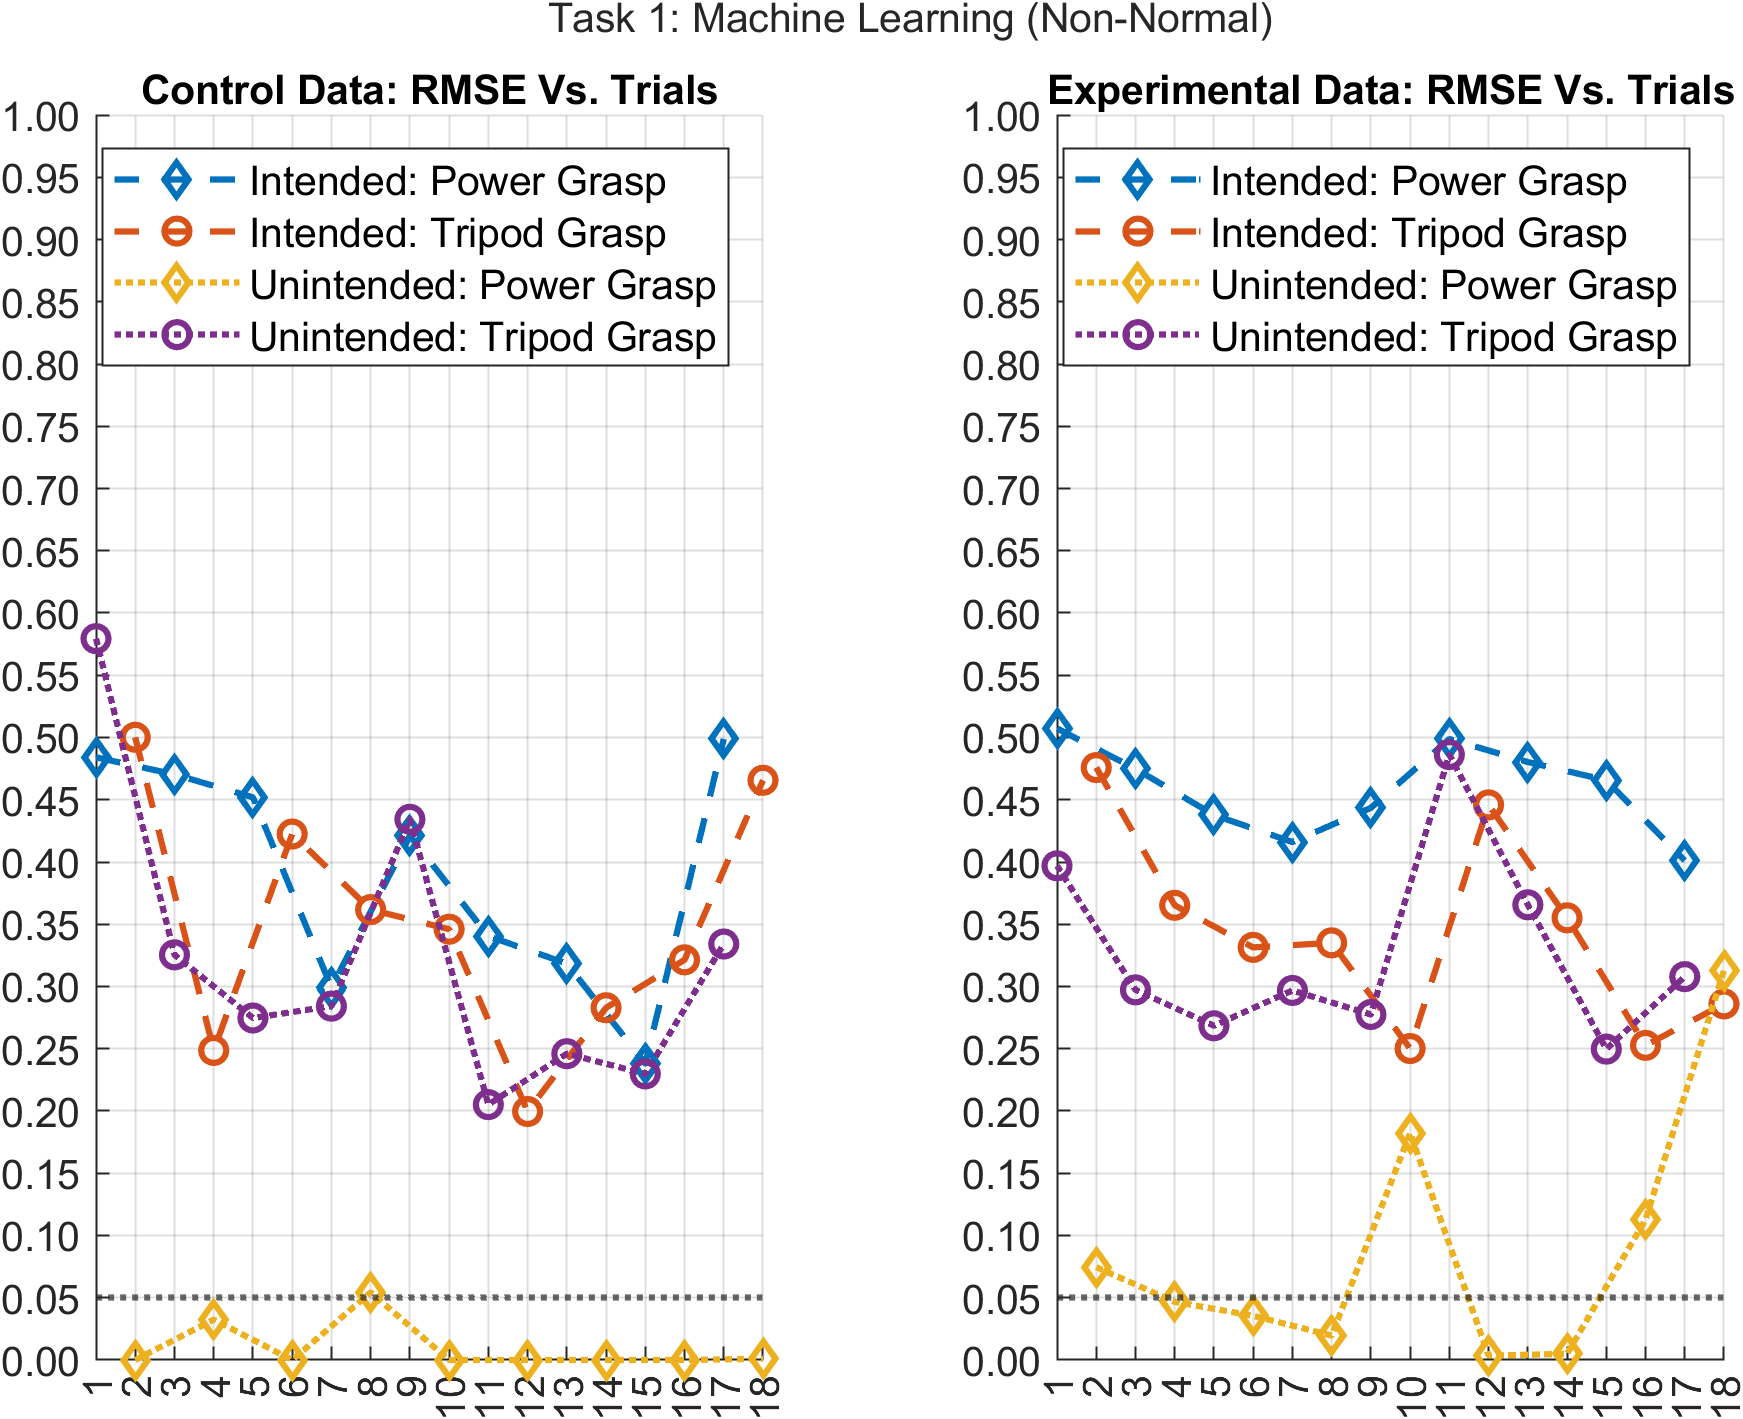
\includegraphics[width = \figWidth]{t1-rmse-xnorm.png}
\end{figure}
\begin{figure}
    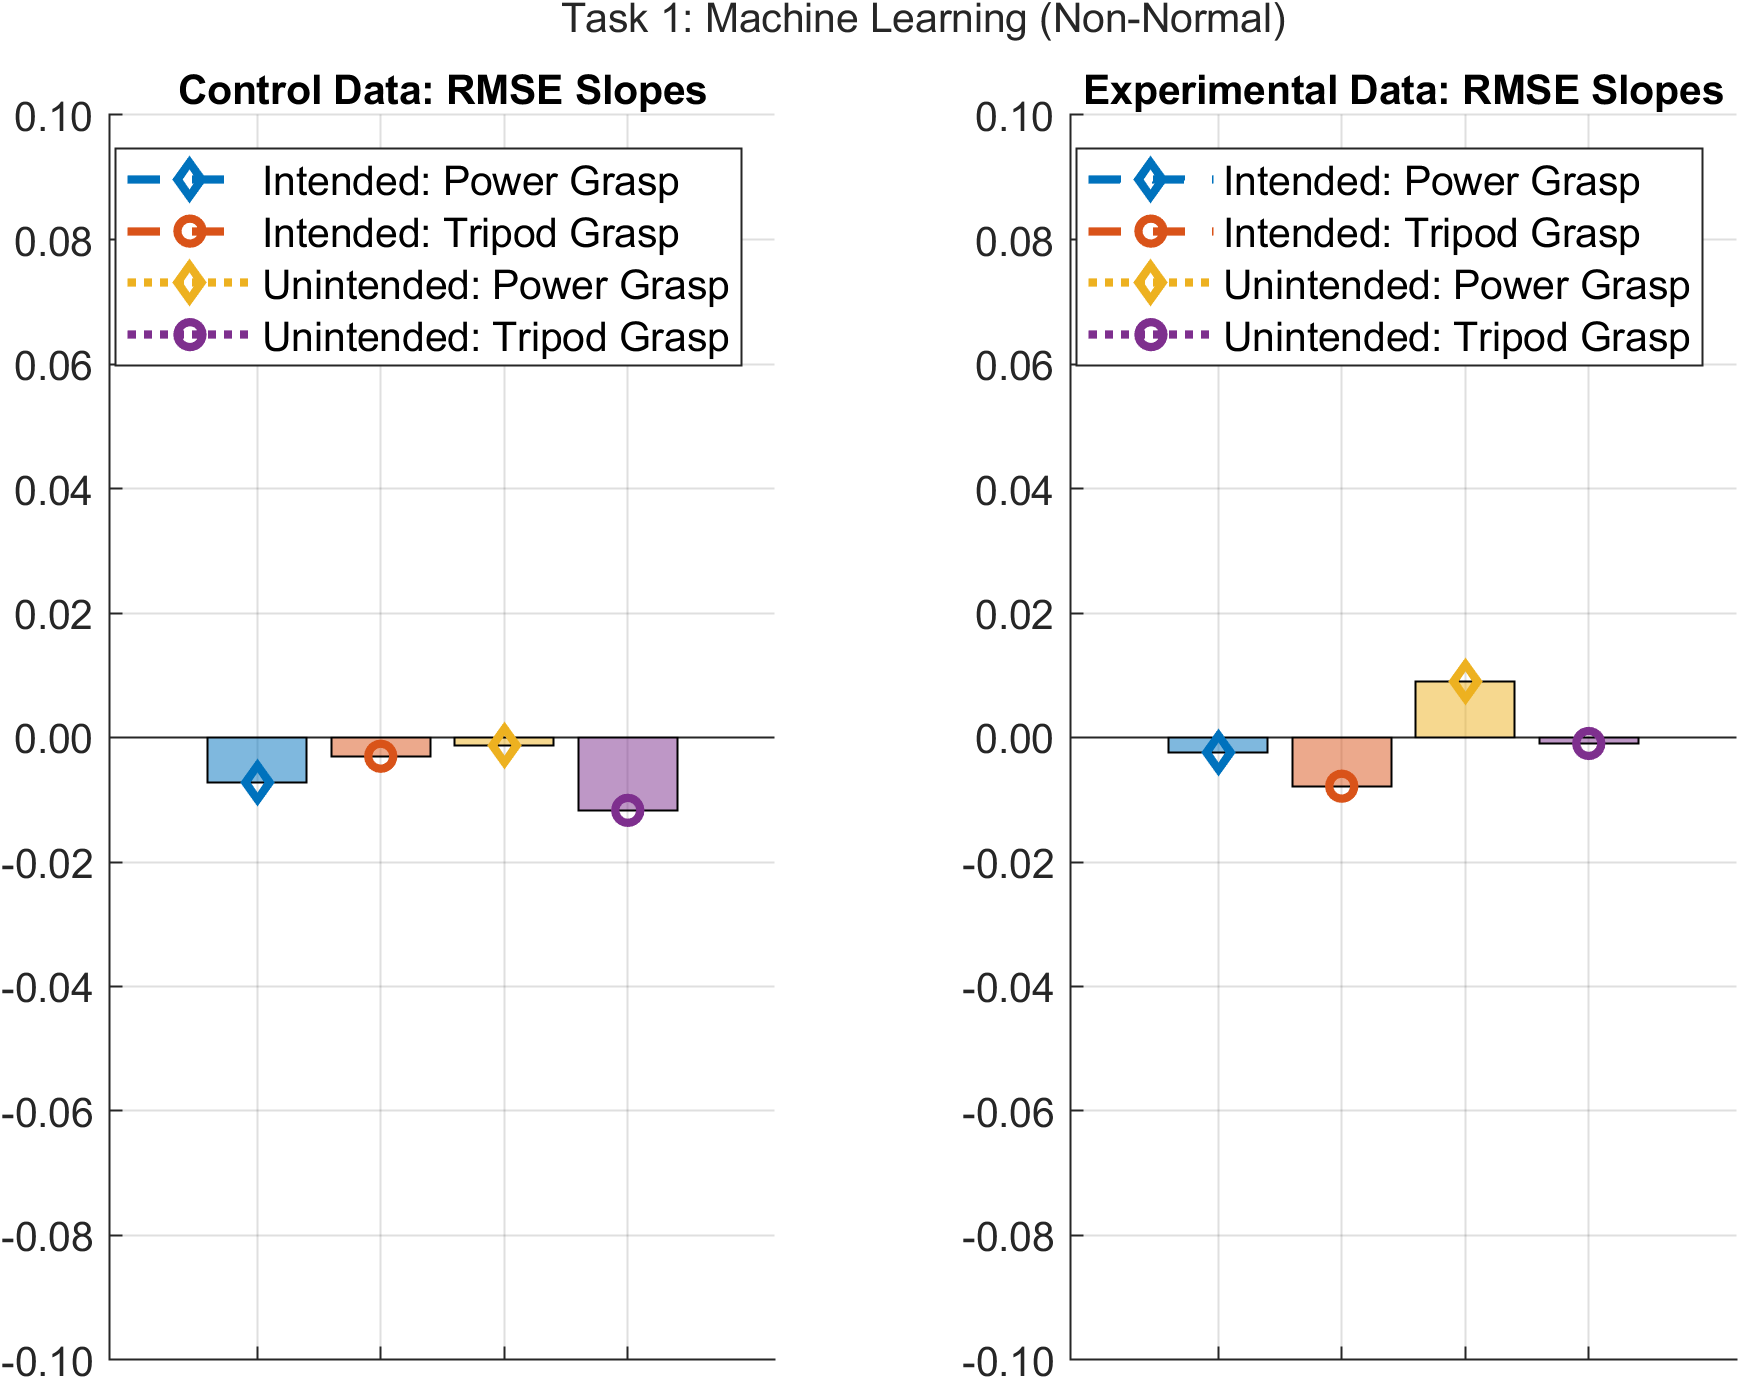
\includegraphics[width = \figWidth]{t1-bar-xnorm.png}
\end{figure}
\begin{figure}
    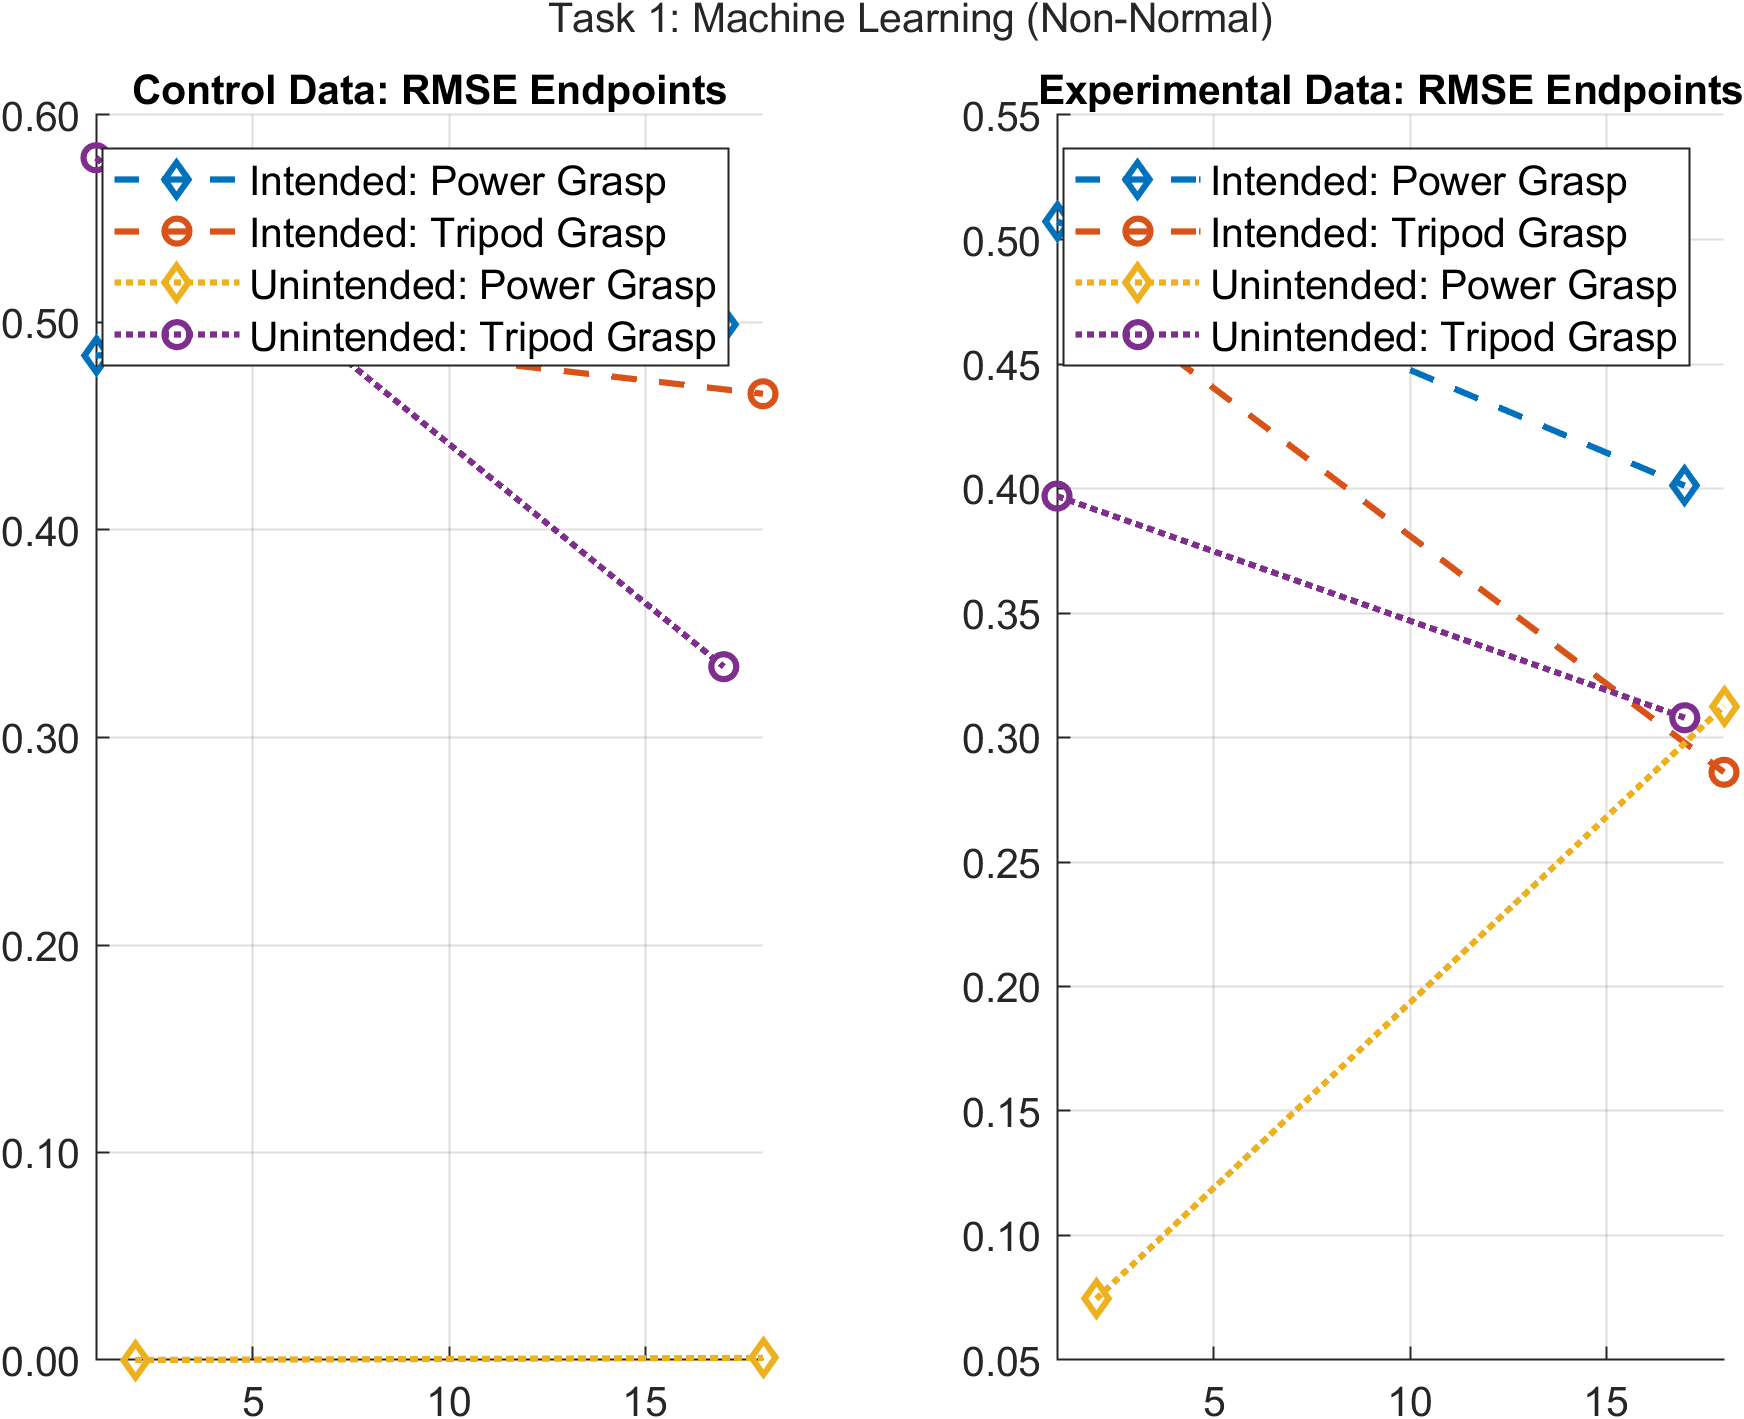
\includegraphics[width = \figWidth]{t1-spaghetti-xnorm.png}
\end{figure}

\begin{figure}
    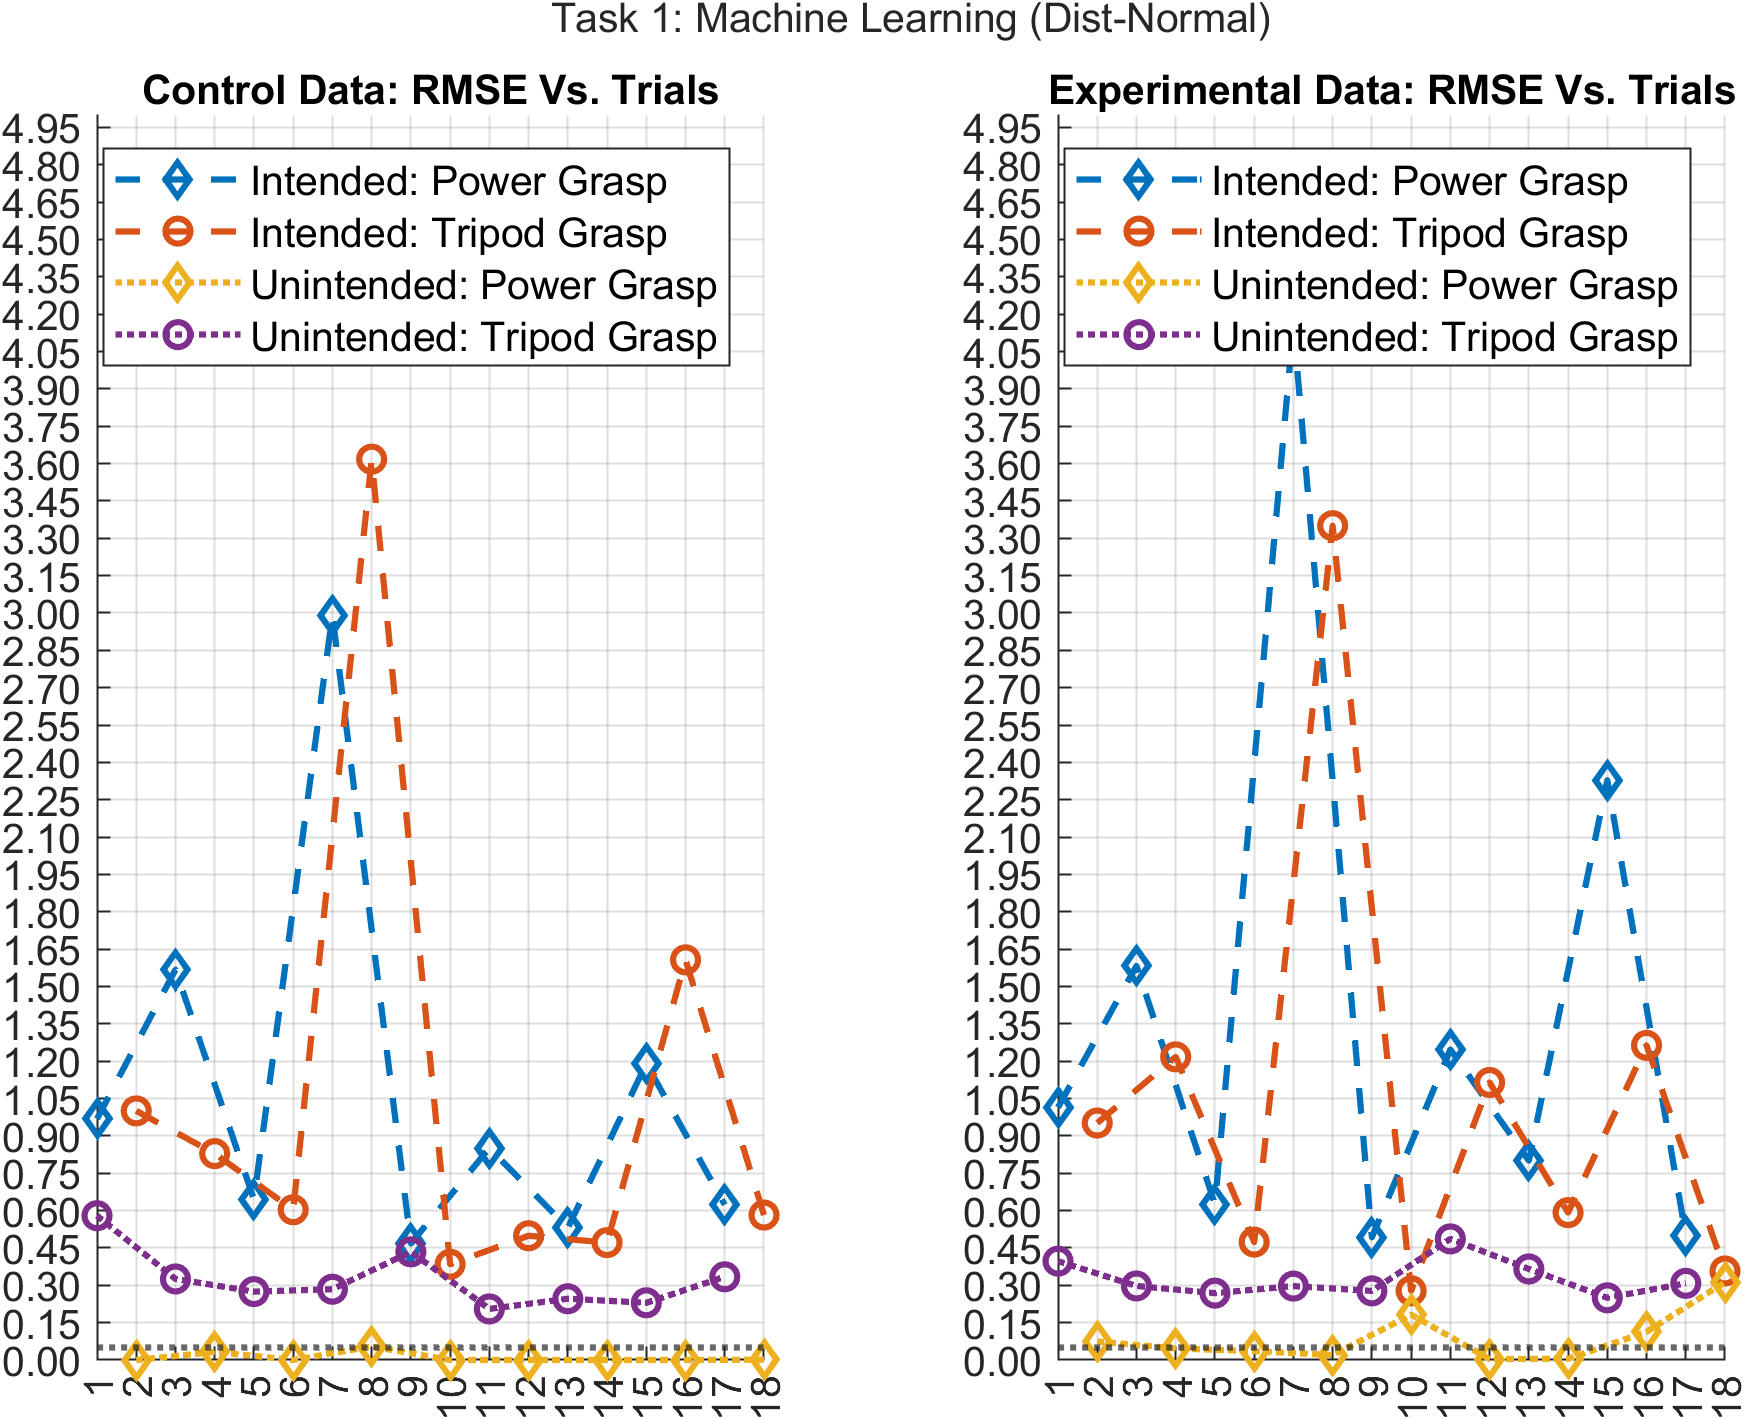
\includegraphics[width = \figWidth]{t1-rmse-dnorm.png}
\end{figure}
\begin{figure}
    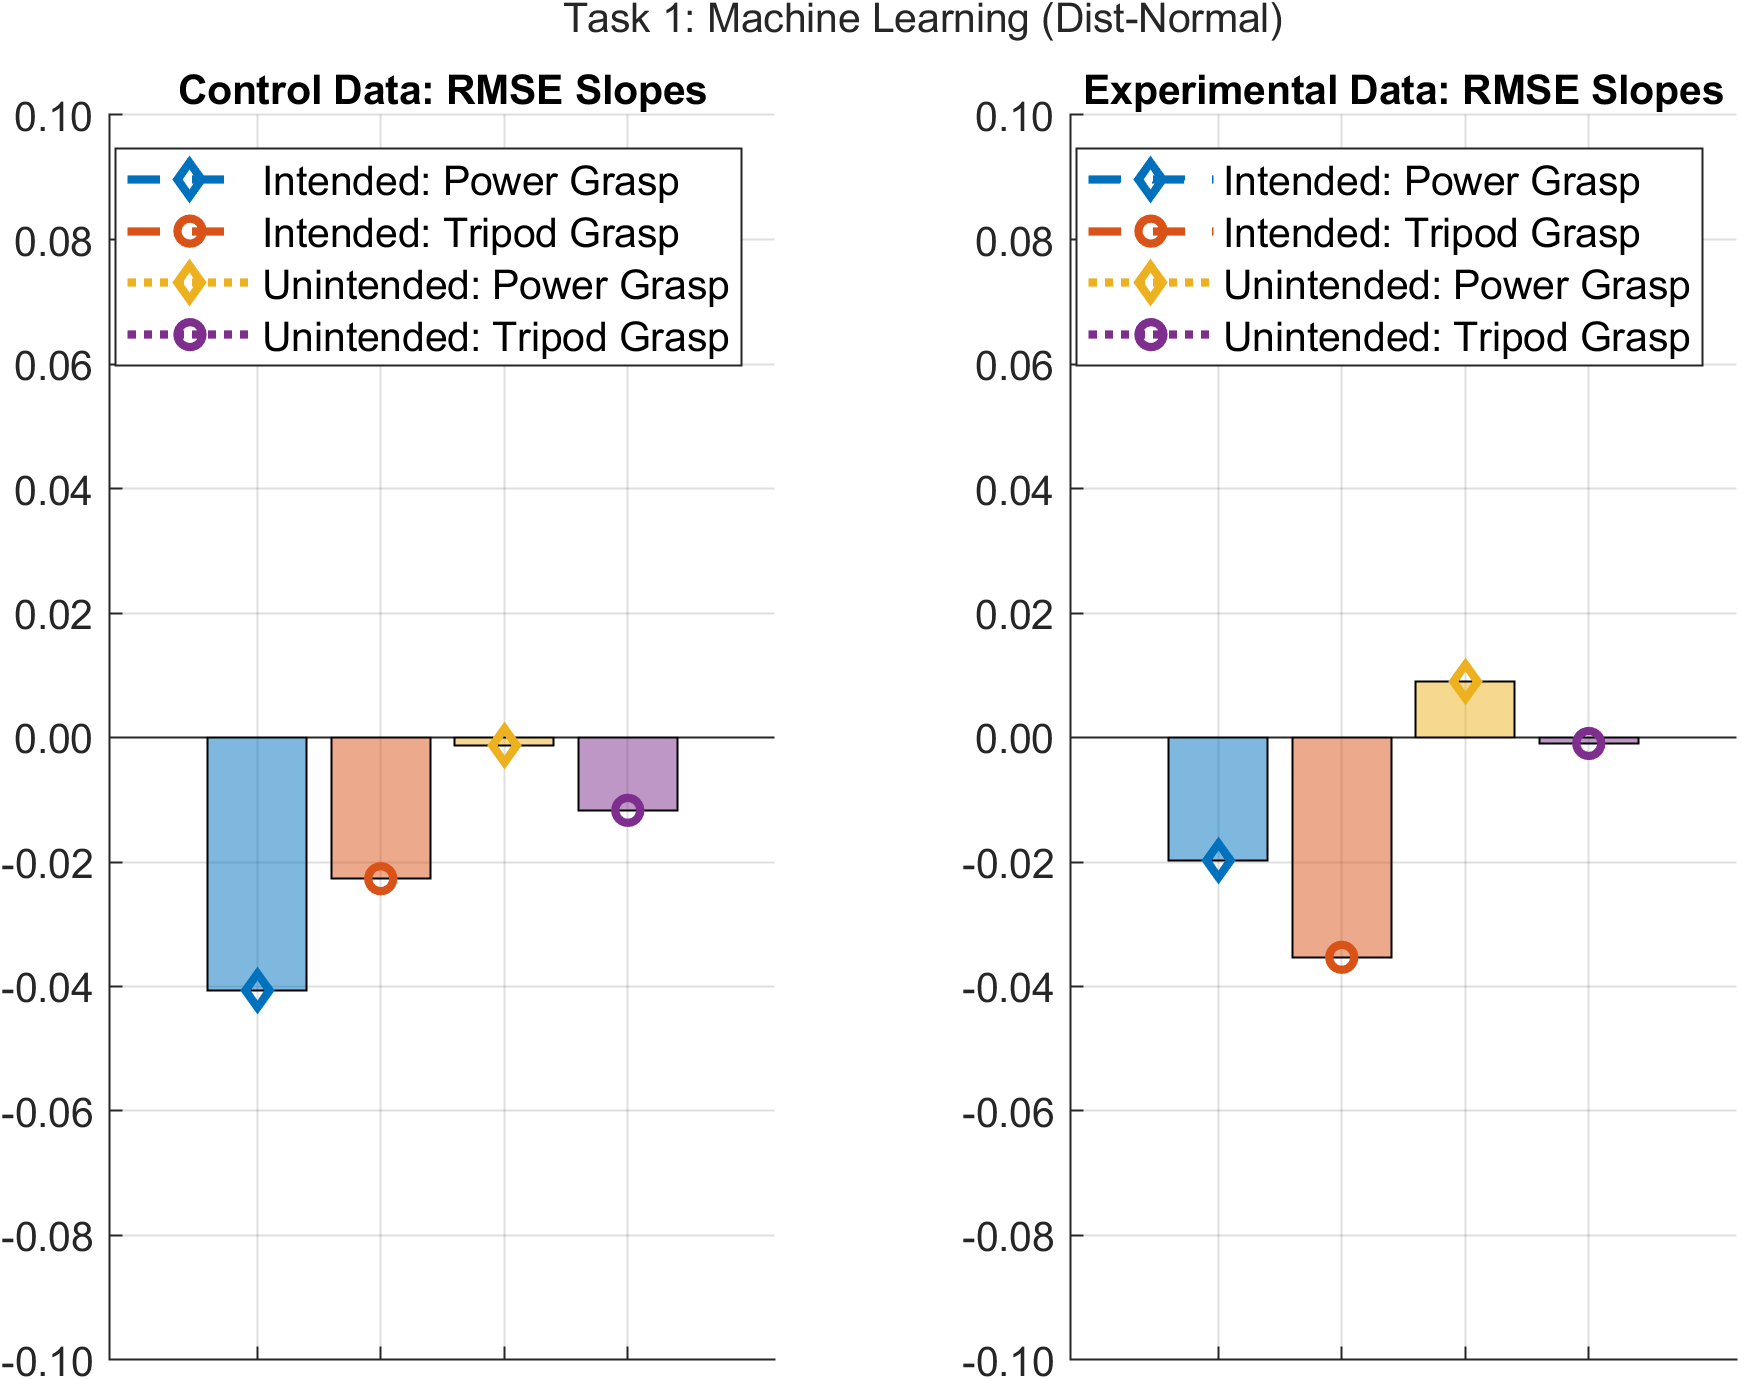
\includegraphics[width = \figWidth]{t1-bar-dnorm.png}
\end{figure}
\begin{figure}
    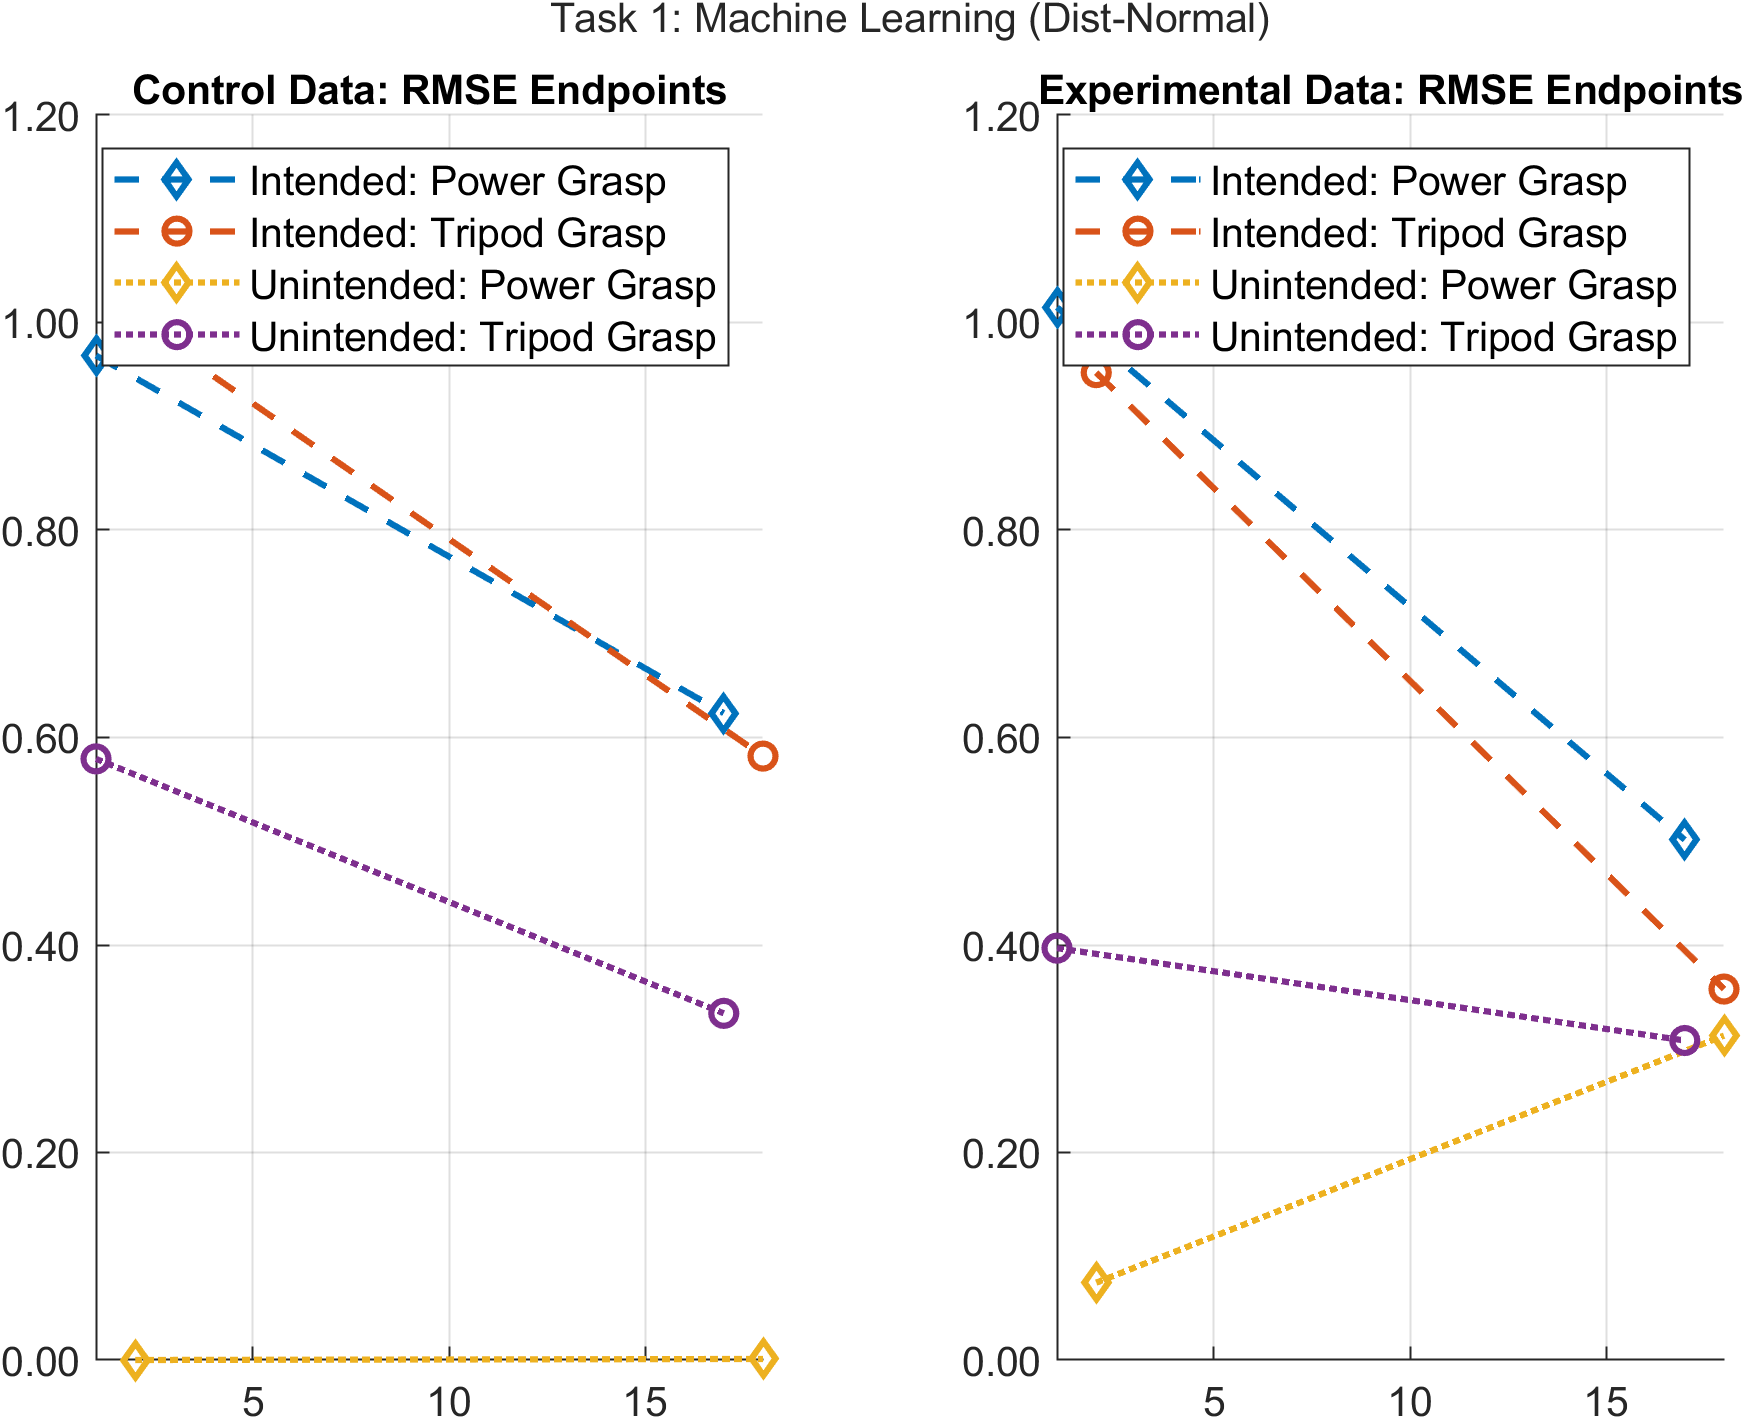
\includegraphics[width = \figWidth]{t1-spaghetti-dnorm.png}
\end{figure}

\begin{figure}
    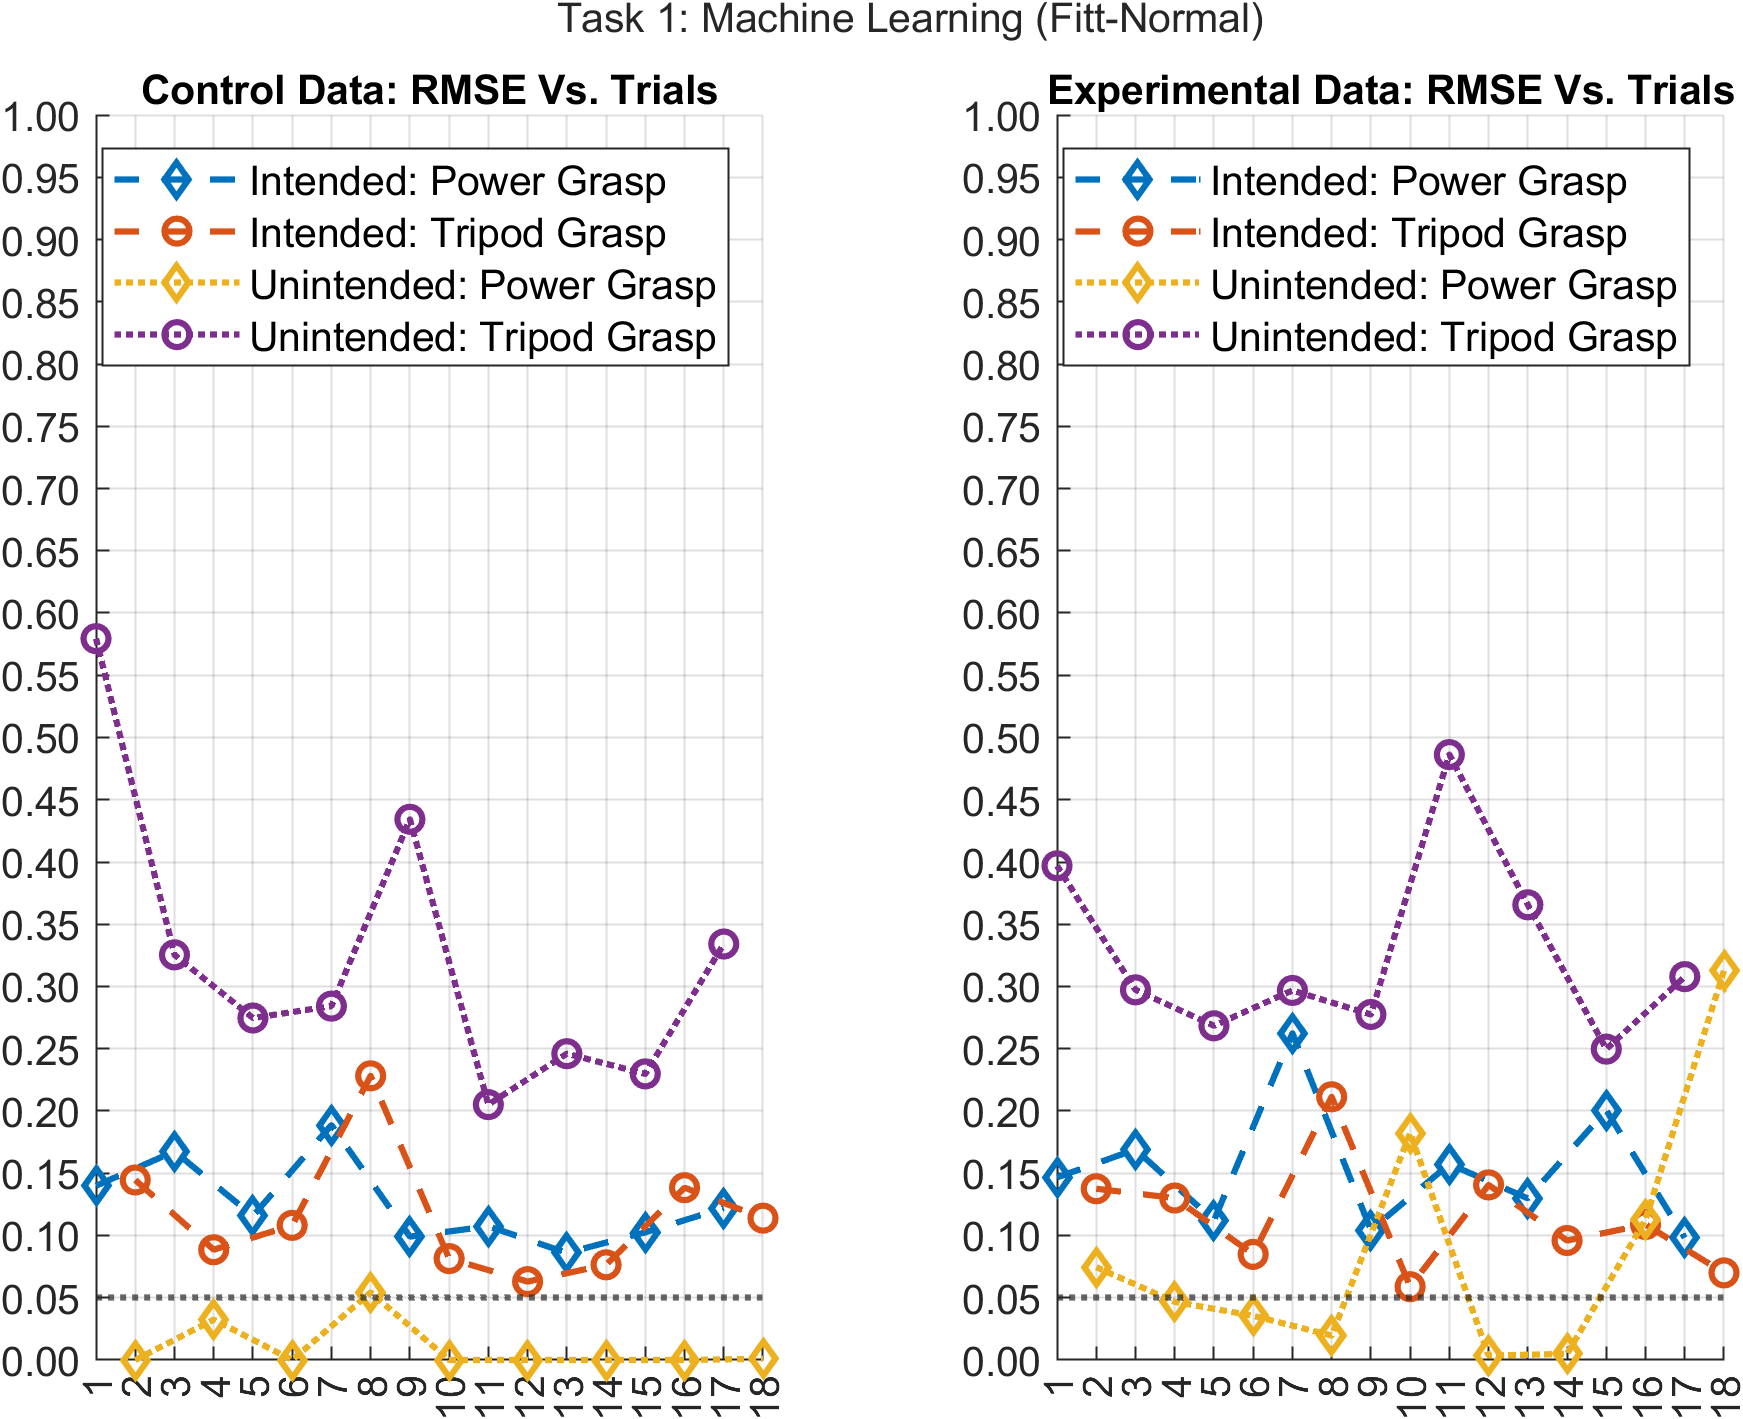
\includegraphics[width = \figWidth]{t1-rmse-fnorm.png}
\end{figure}
\begin{figure}
    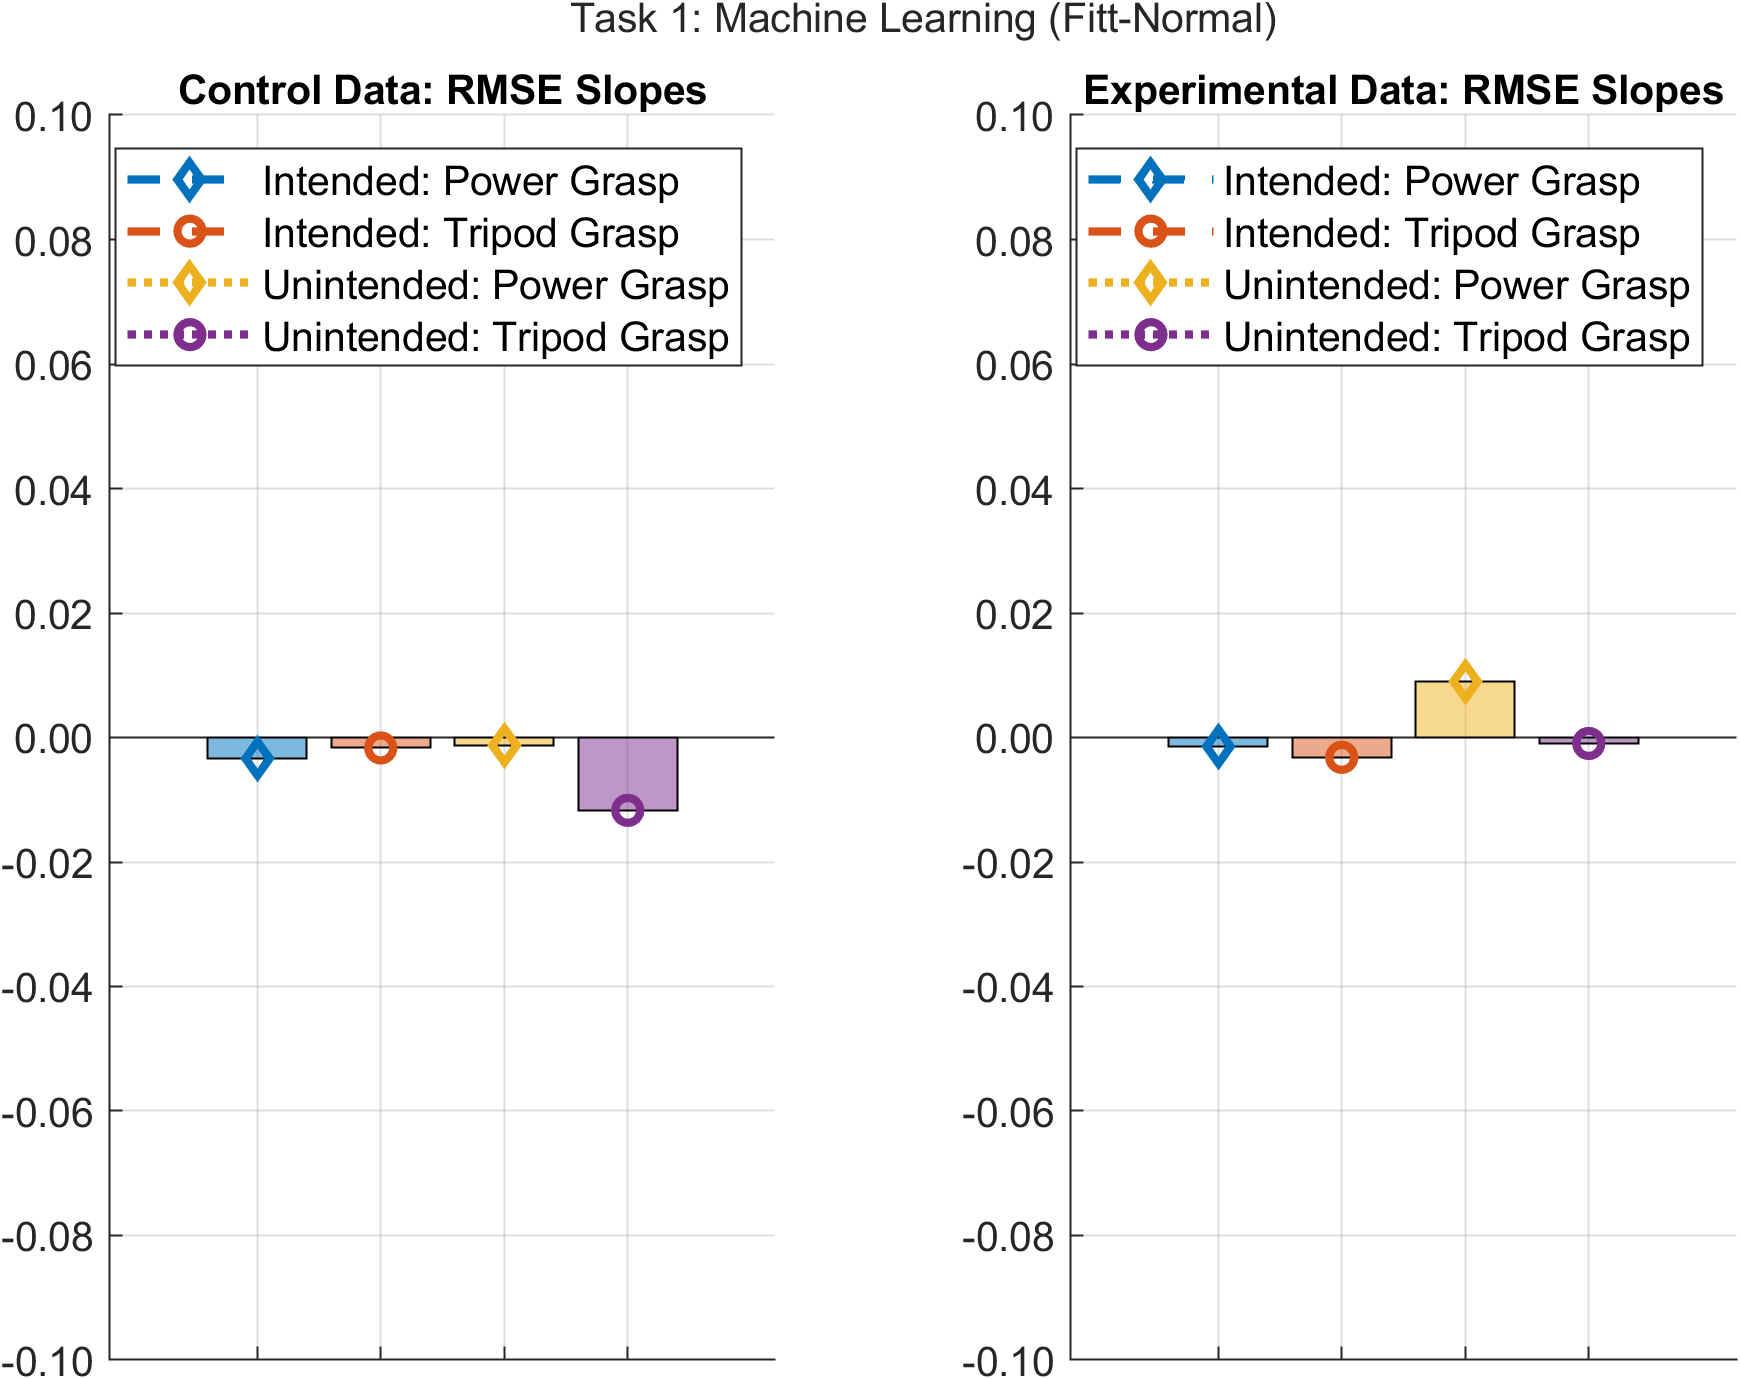
\includegraphics[width = \figWidth]{t1-bar-fnorm.png}
\end{figure}
\begin{figure}
    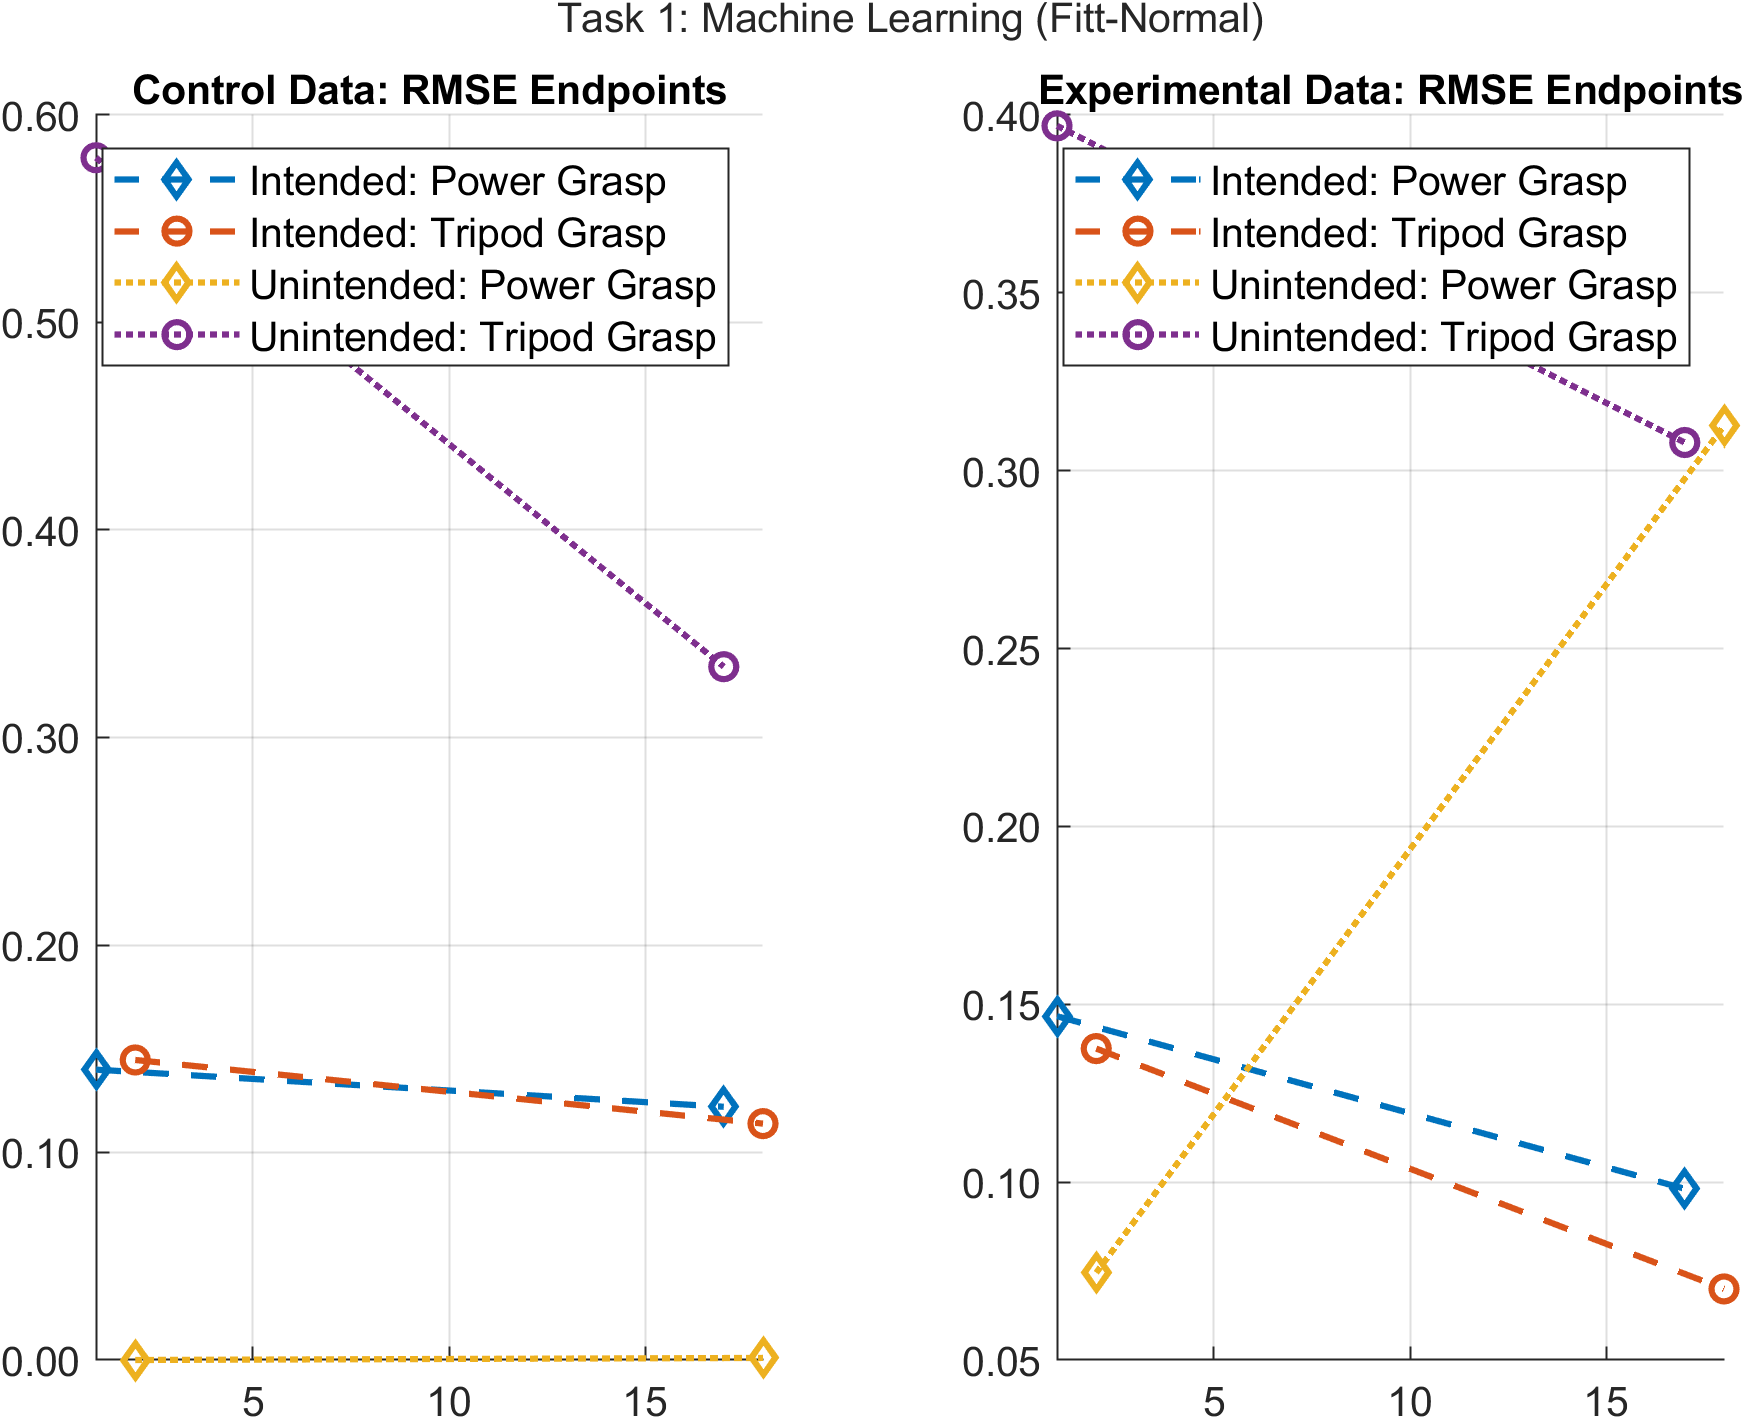
\includegraphics[width = \figWidth]{t1-spaghetti-fnorm.png}
\end{figure}
%%%%%%%%%%%%%%%
\begin{landscape}
    \begin{figure}
        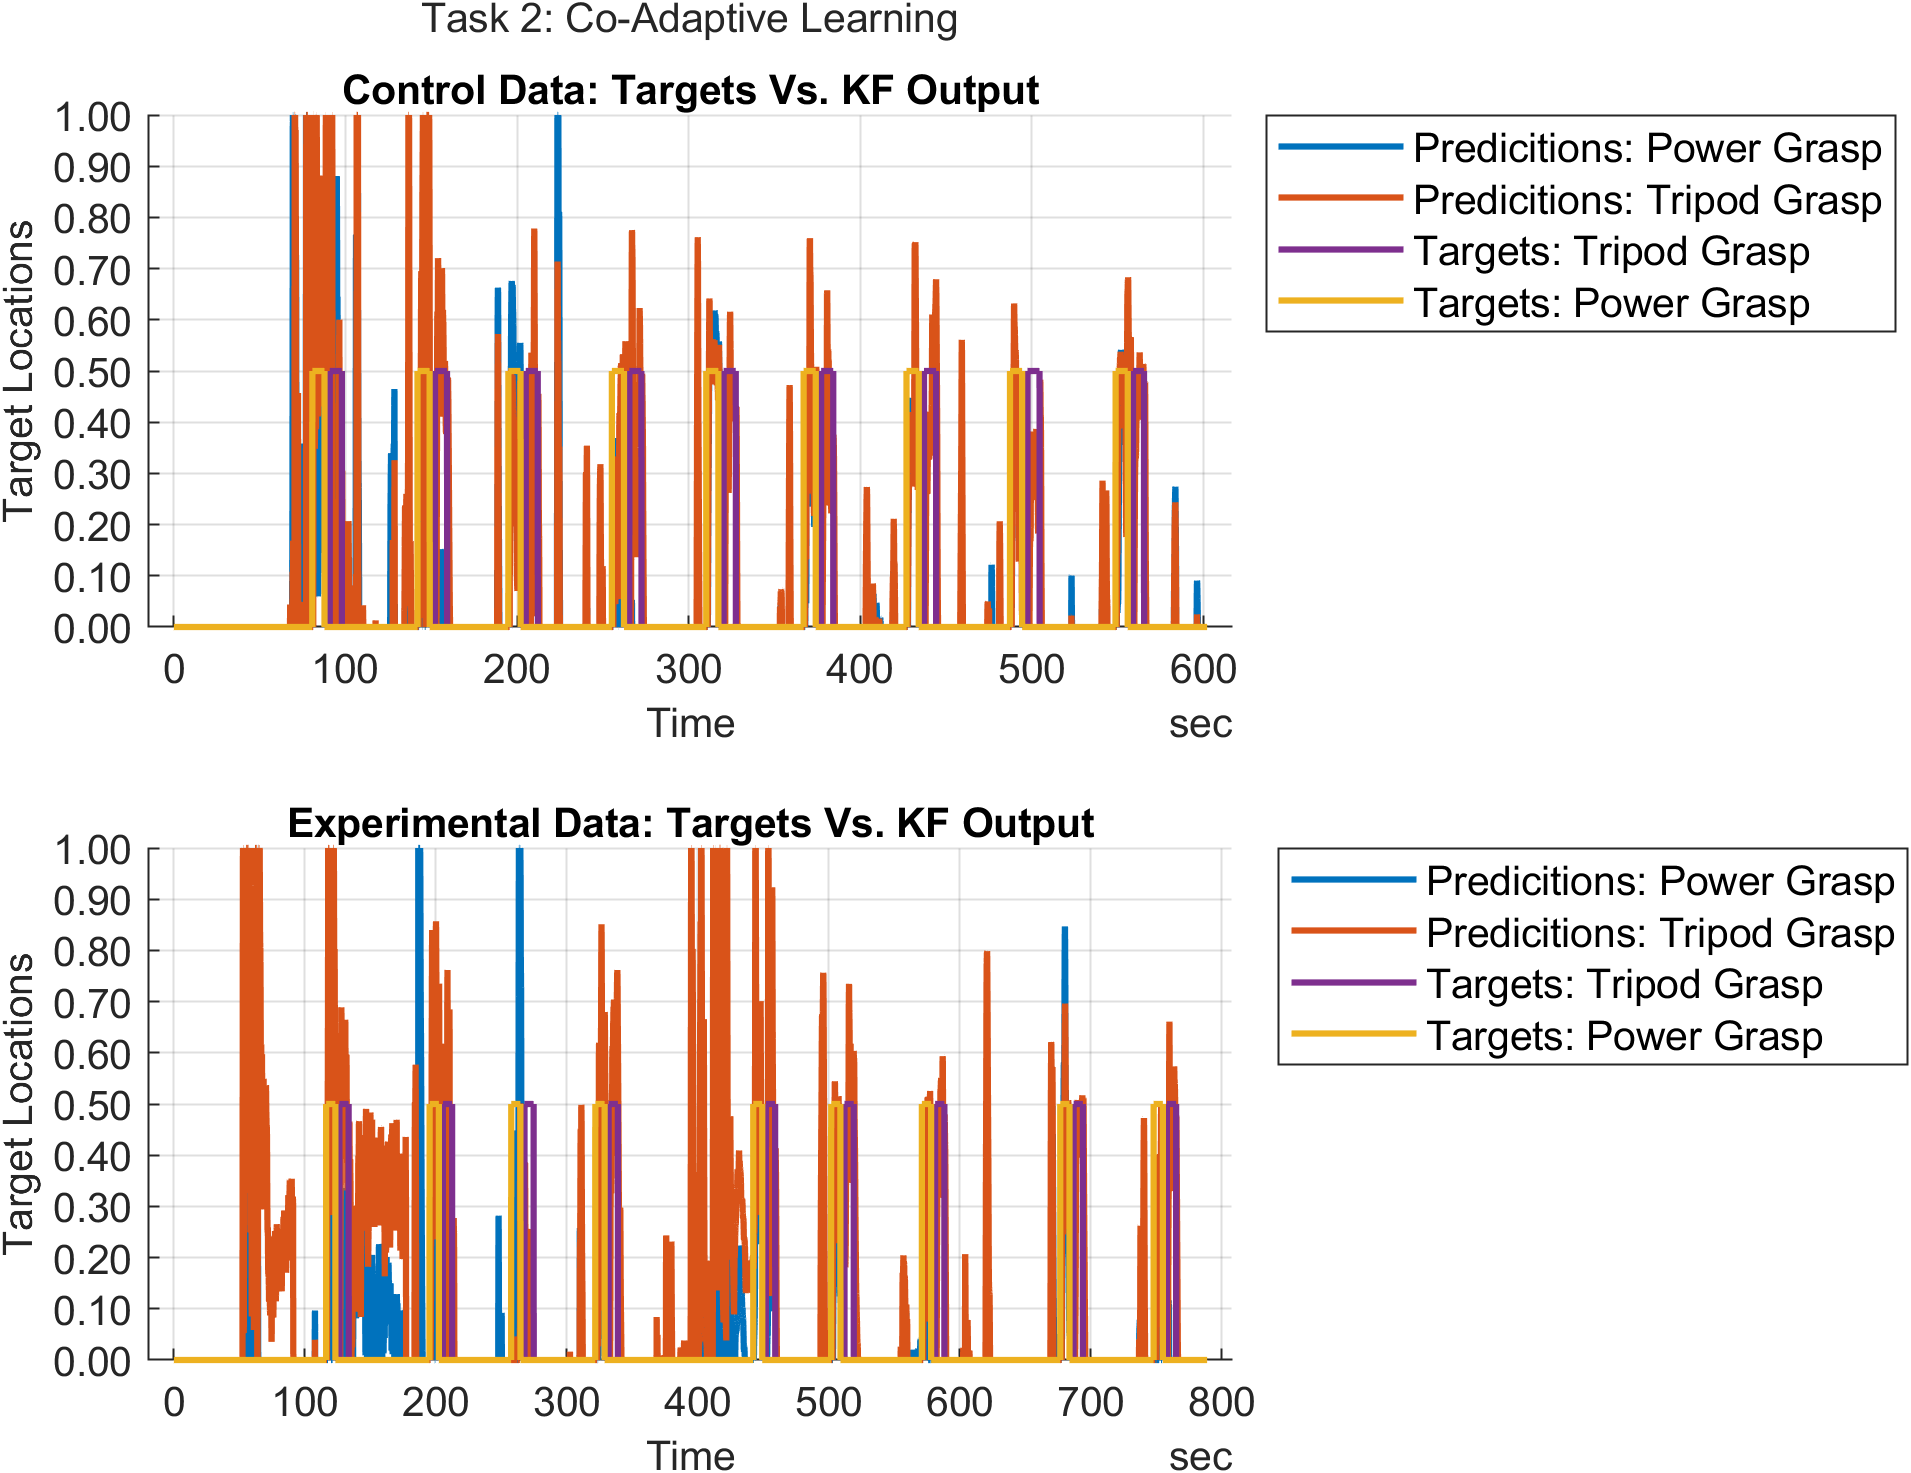
\includegraphics[width = \figWidthLarge]{t2-kf-out.png}
    \end{figure}
\end{landscape}
\begin{figure}
    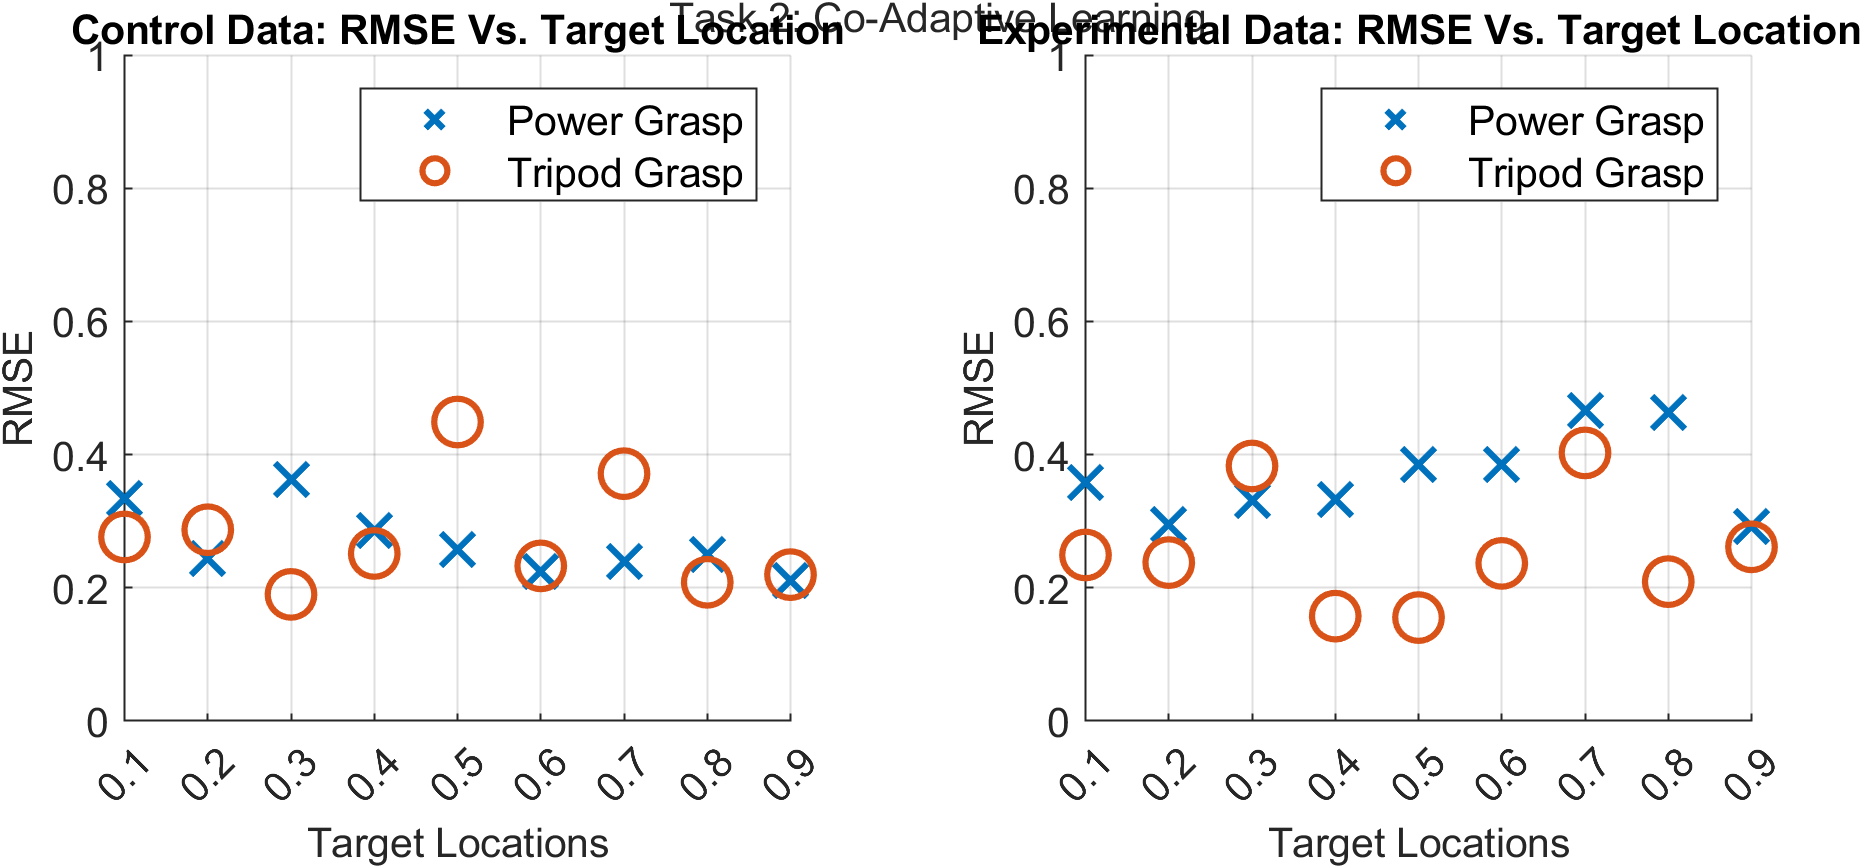
\includegraphics[width = \figWidth]{t2-rmse-reg.png}
\end{figure}
\newpage
\clearpage
\begin{figure}
    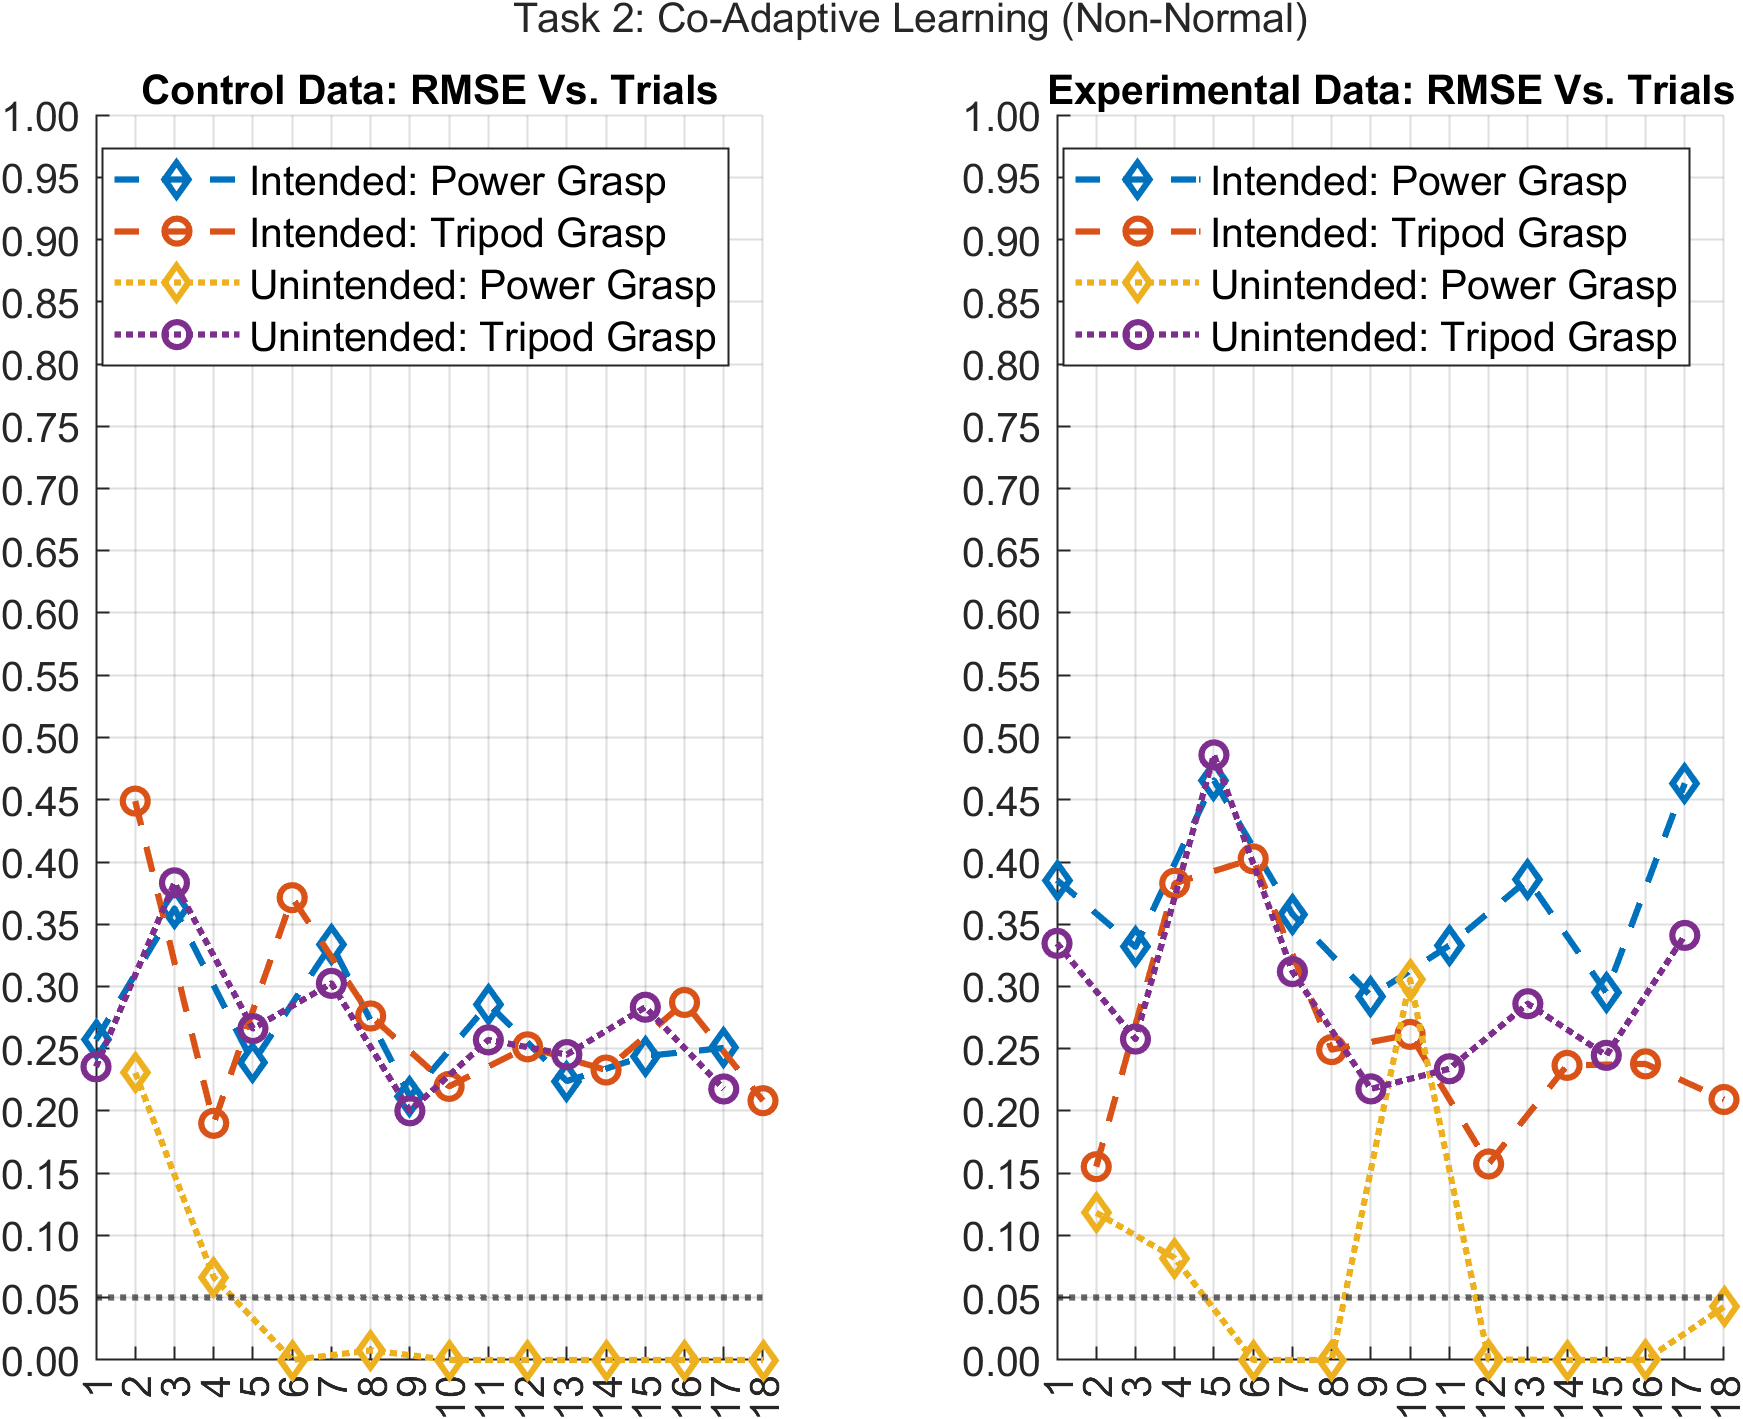
\includegraphics[width = \figWidth]{t2-rmse-xnorm.png}
\end{figure}
\begin{figure}
    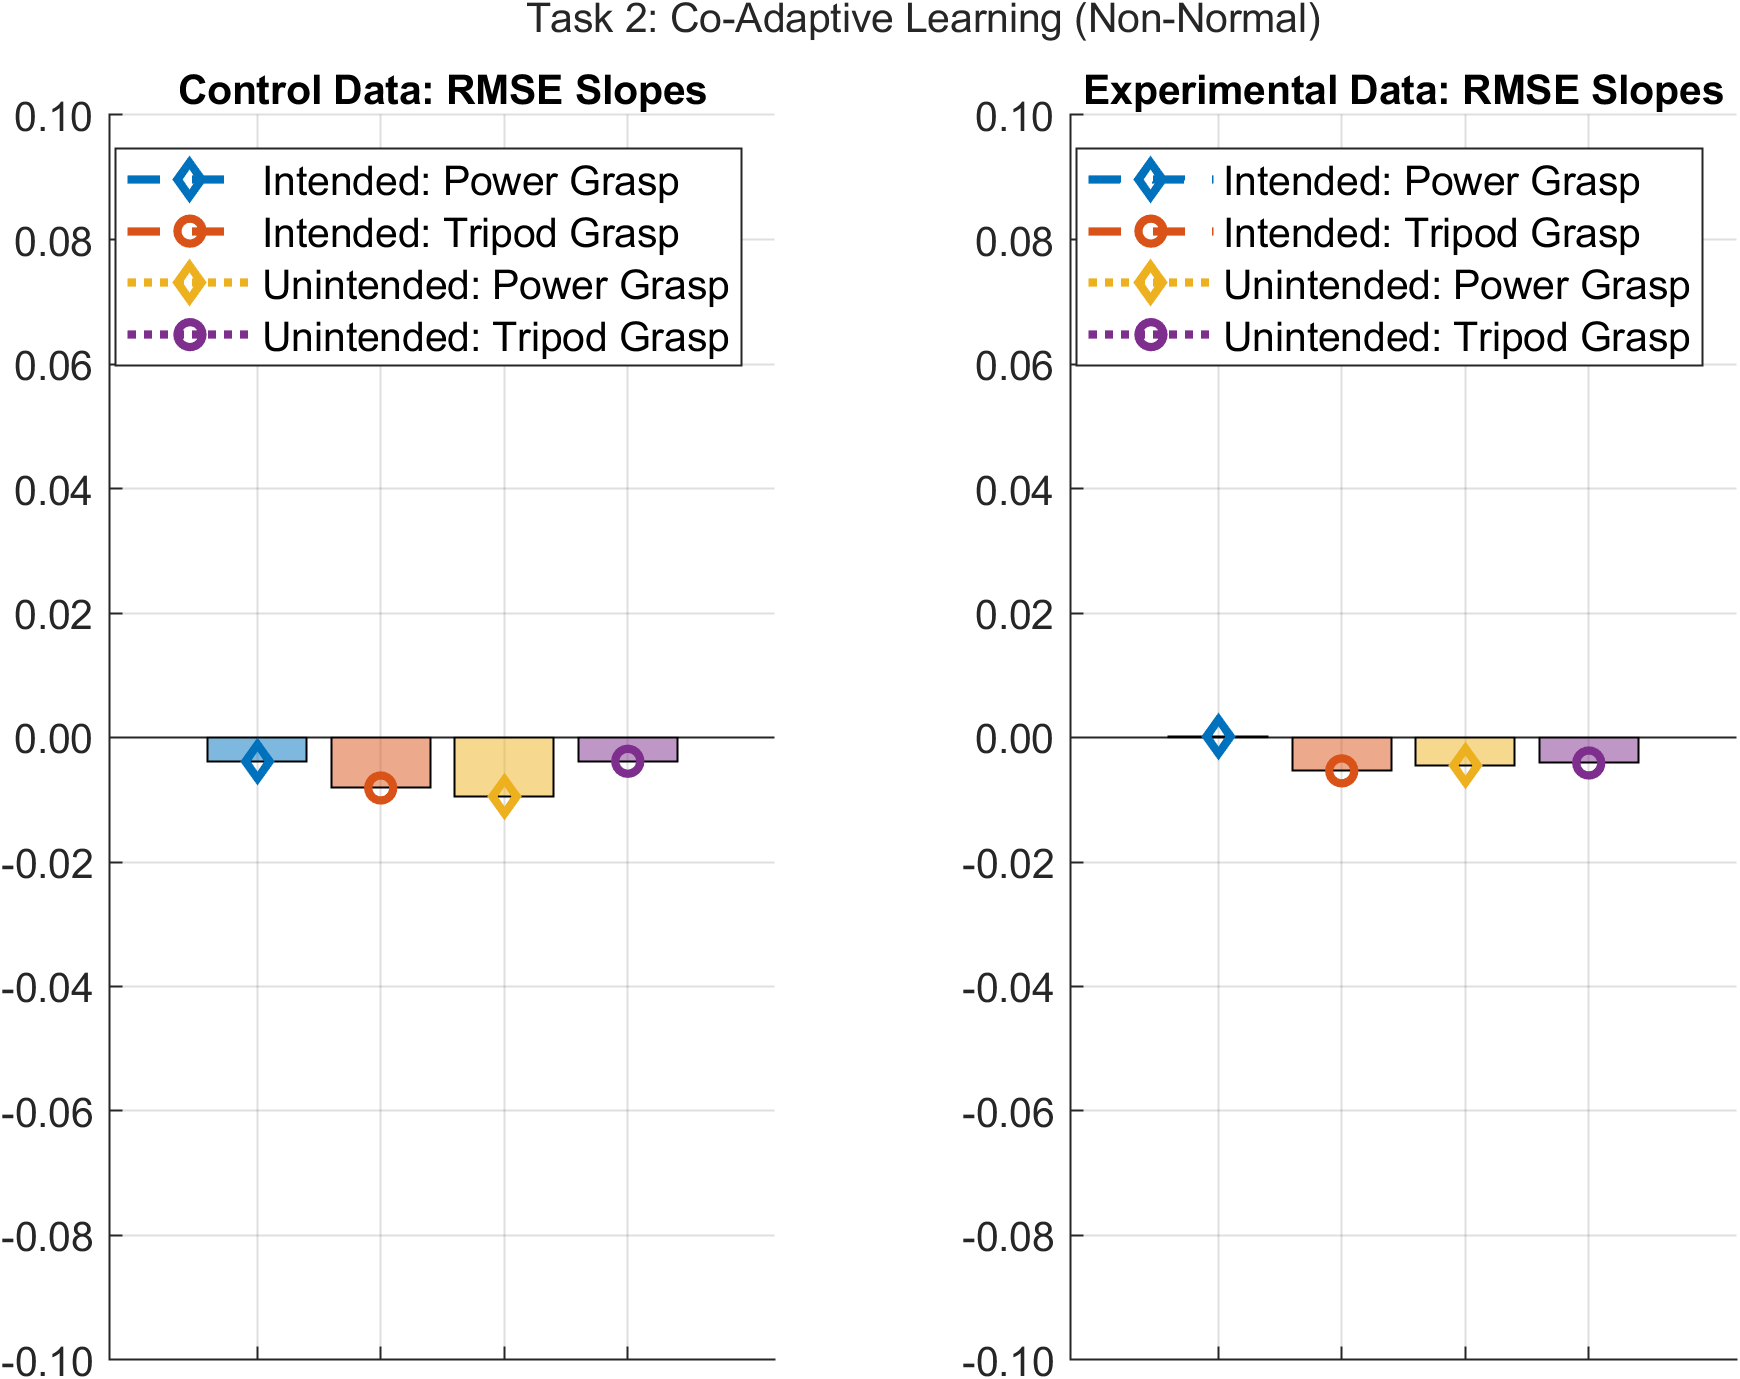
\includegraphics[width = \figWidth]{t2-bar-xnorm.png}
\end{figure}
\begin{figure}
    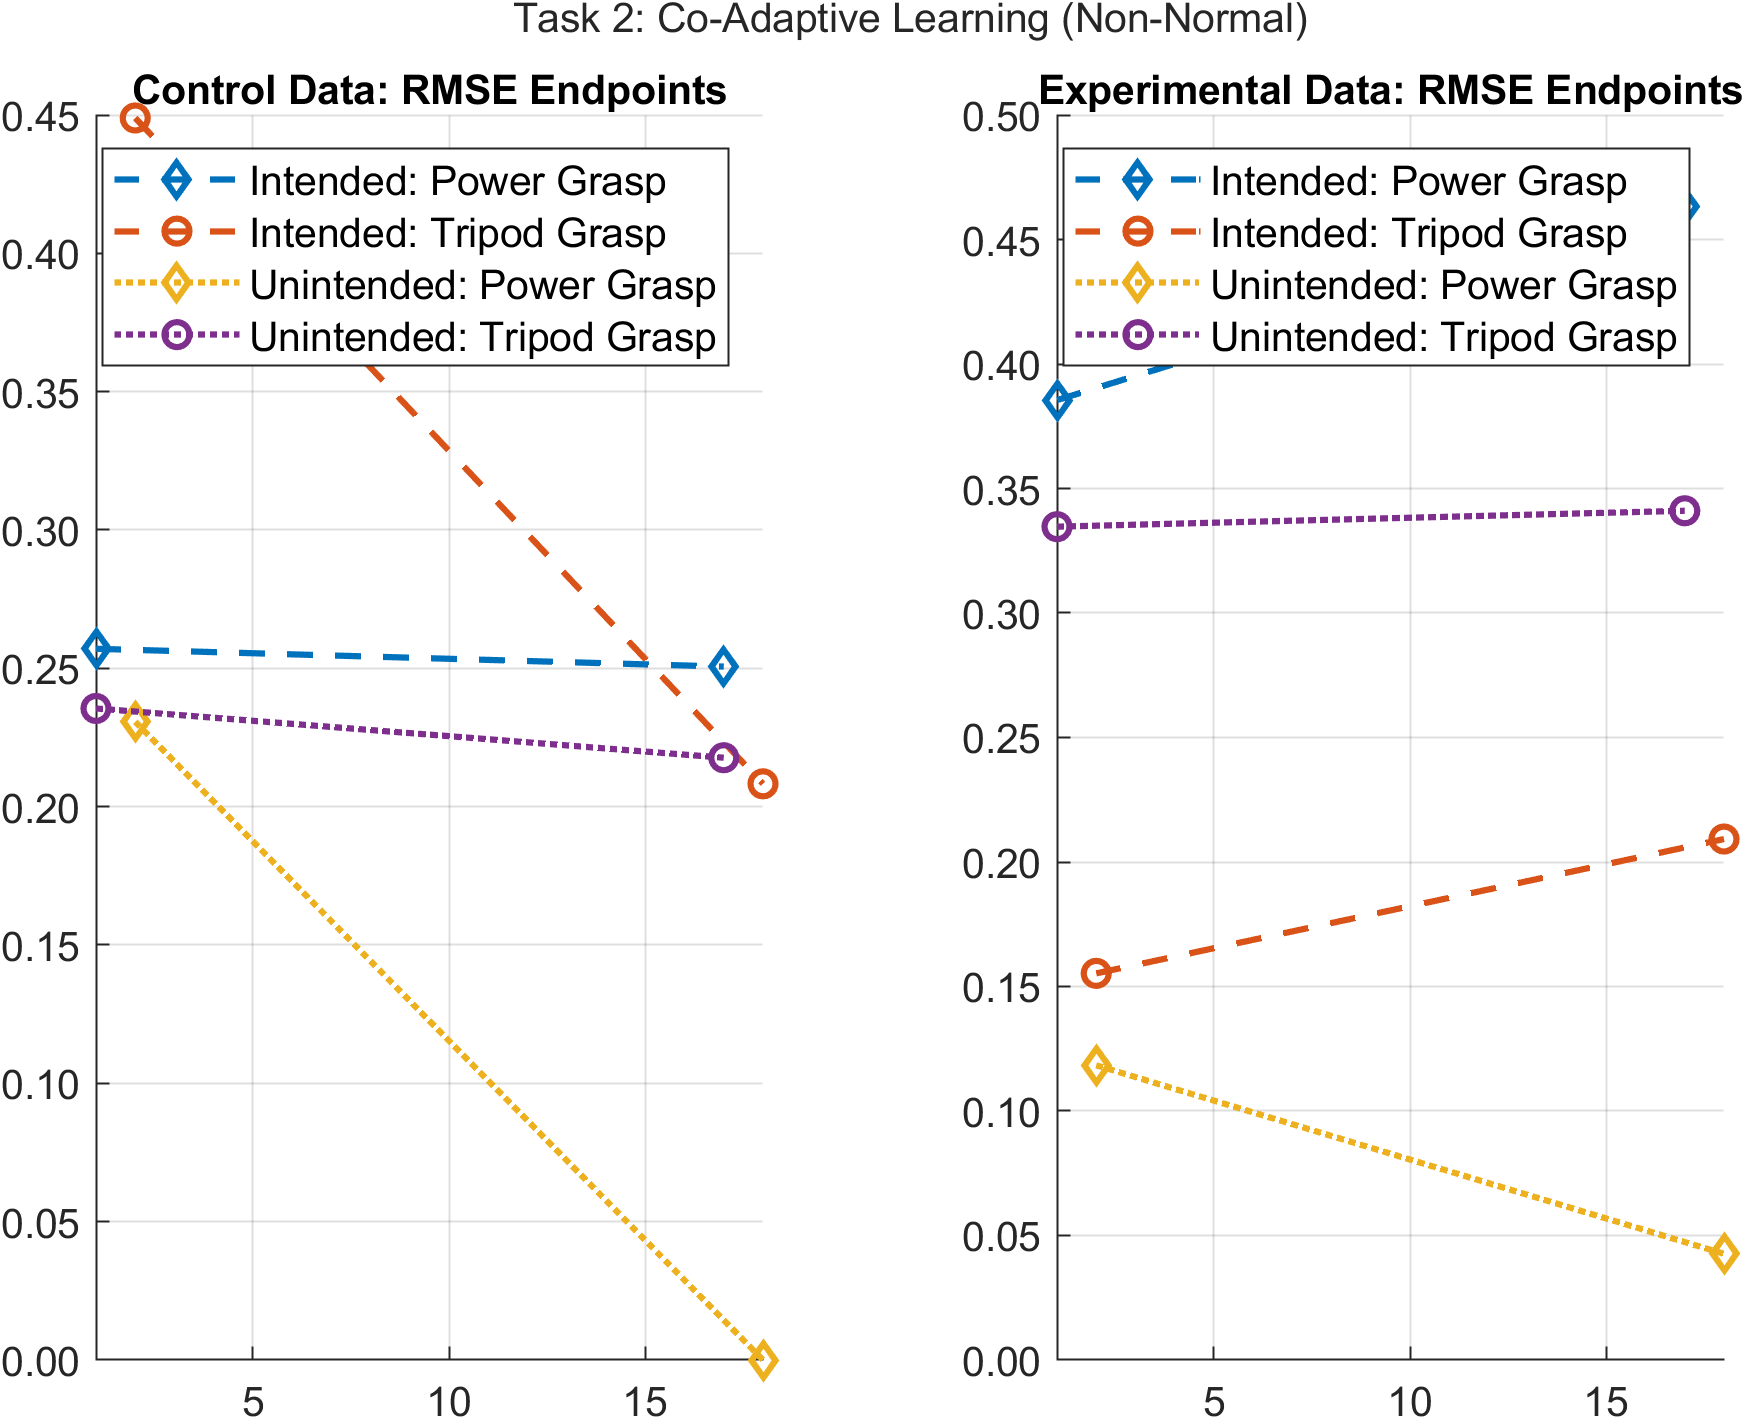
\includegraphics[width = \figWidth]{t2-spaghetti-xnorm.png}
\end{figure}

\begin{figure}
    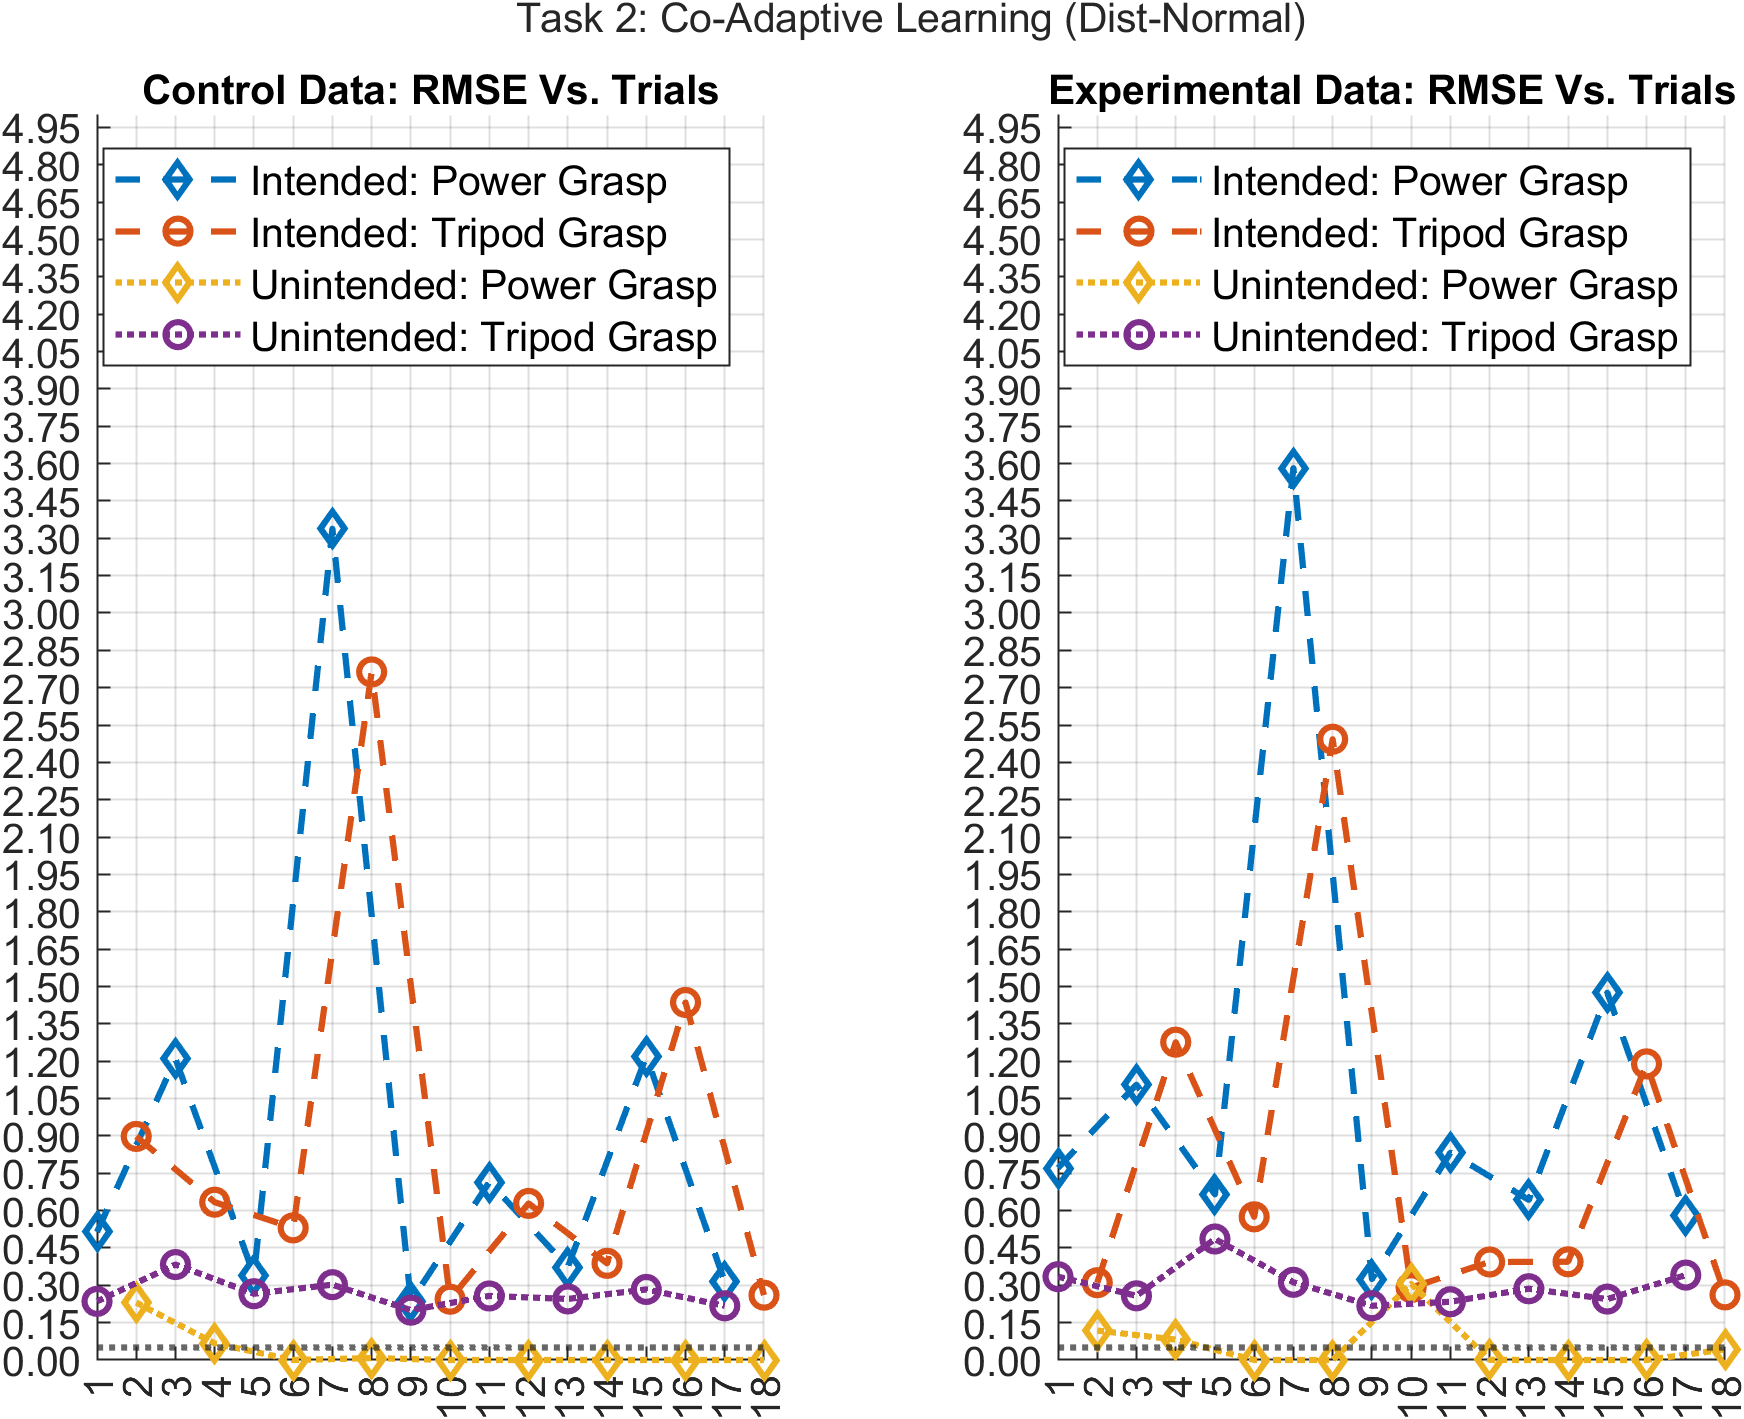
\includegraphics[width = \figWidth]{t2-rmse-dnorm.png}
\end{figure}
\begin{figure}
    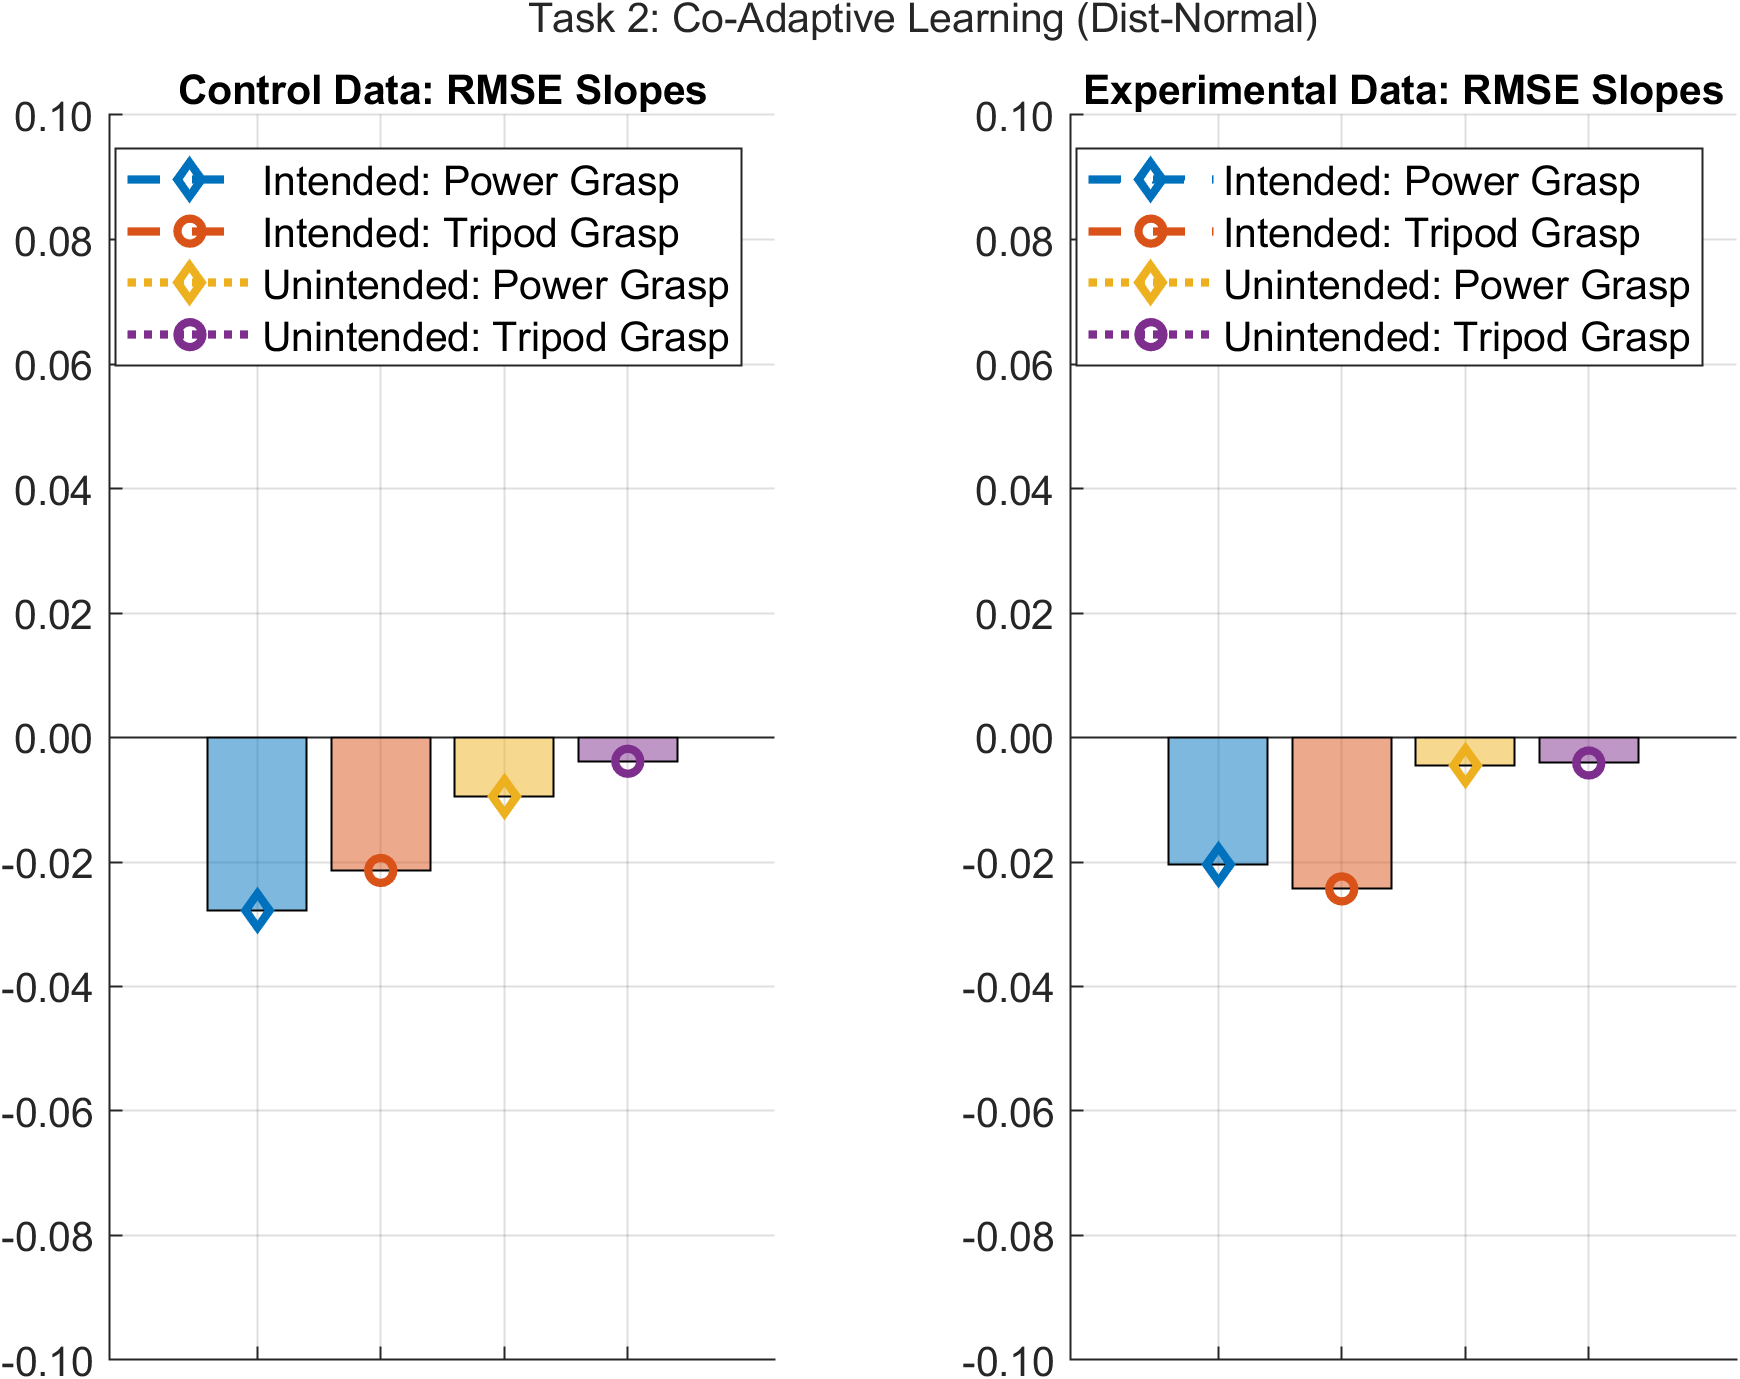
\includegraphics[width = \figWidth]{t2-bar-dnorm.png}
\end{figure}
\begin{figure}
    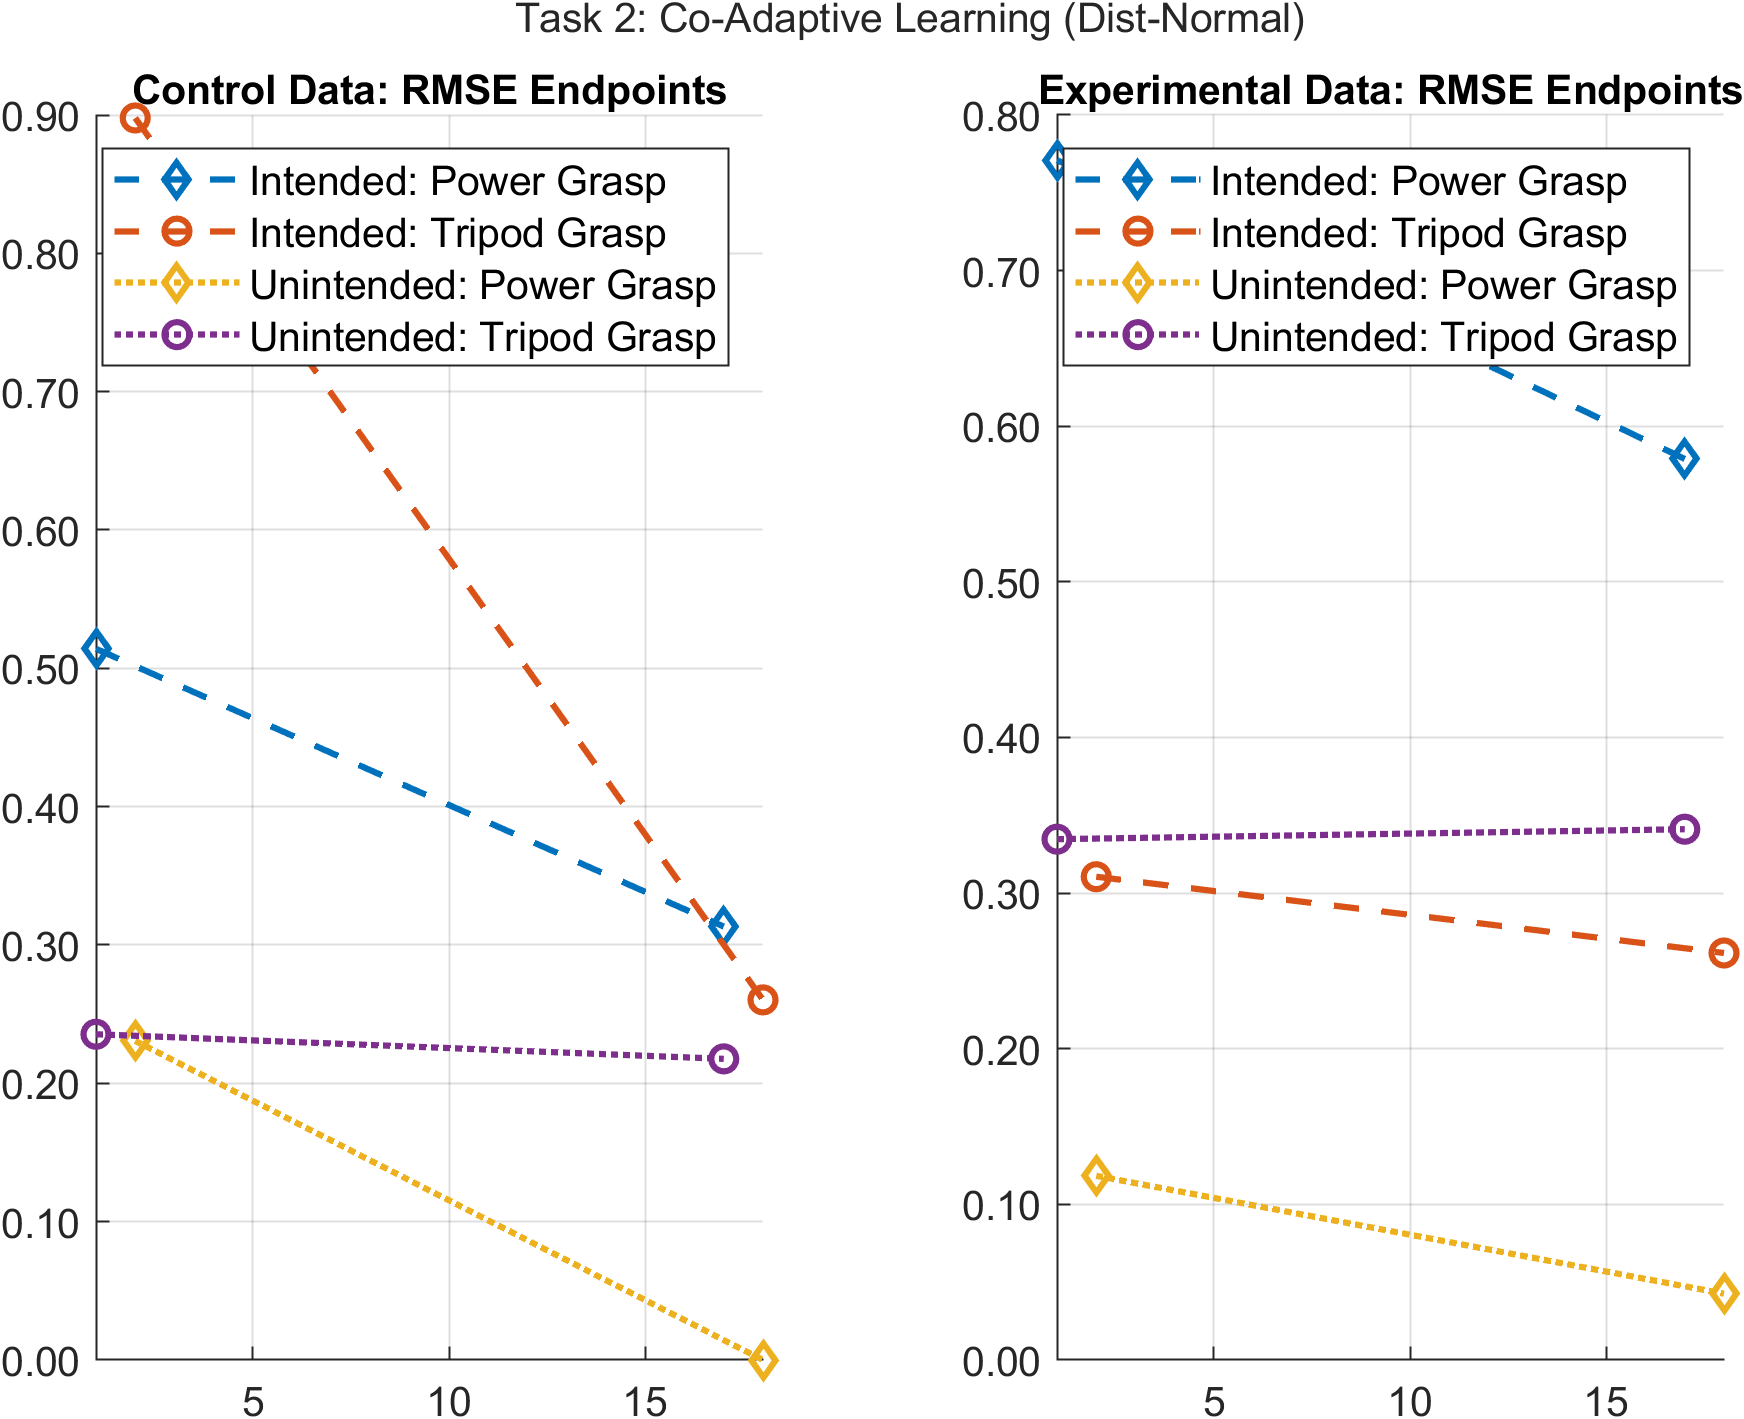
\includegraphics[width = \figWidth]{t2-spaghetti-dnorm.png}
\end{figure}

\begin{figure}
    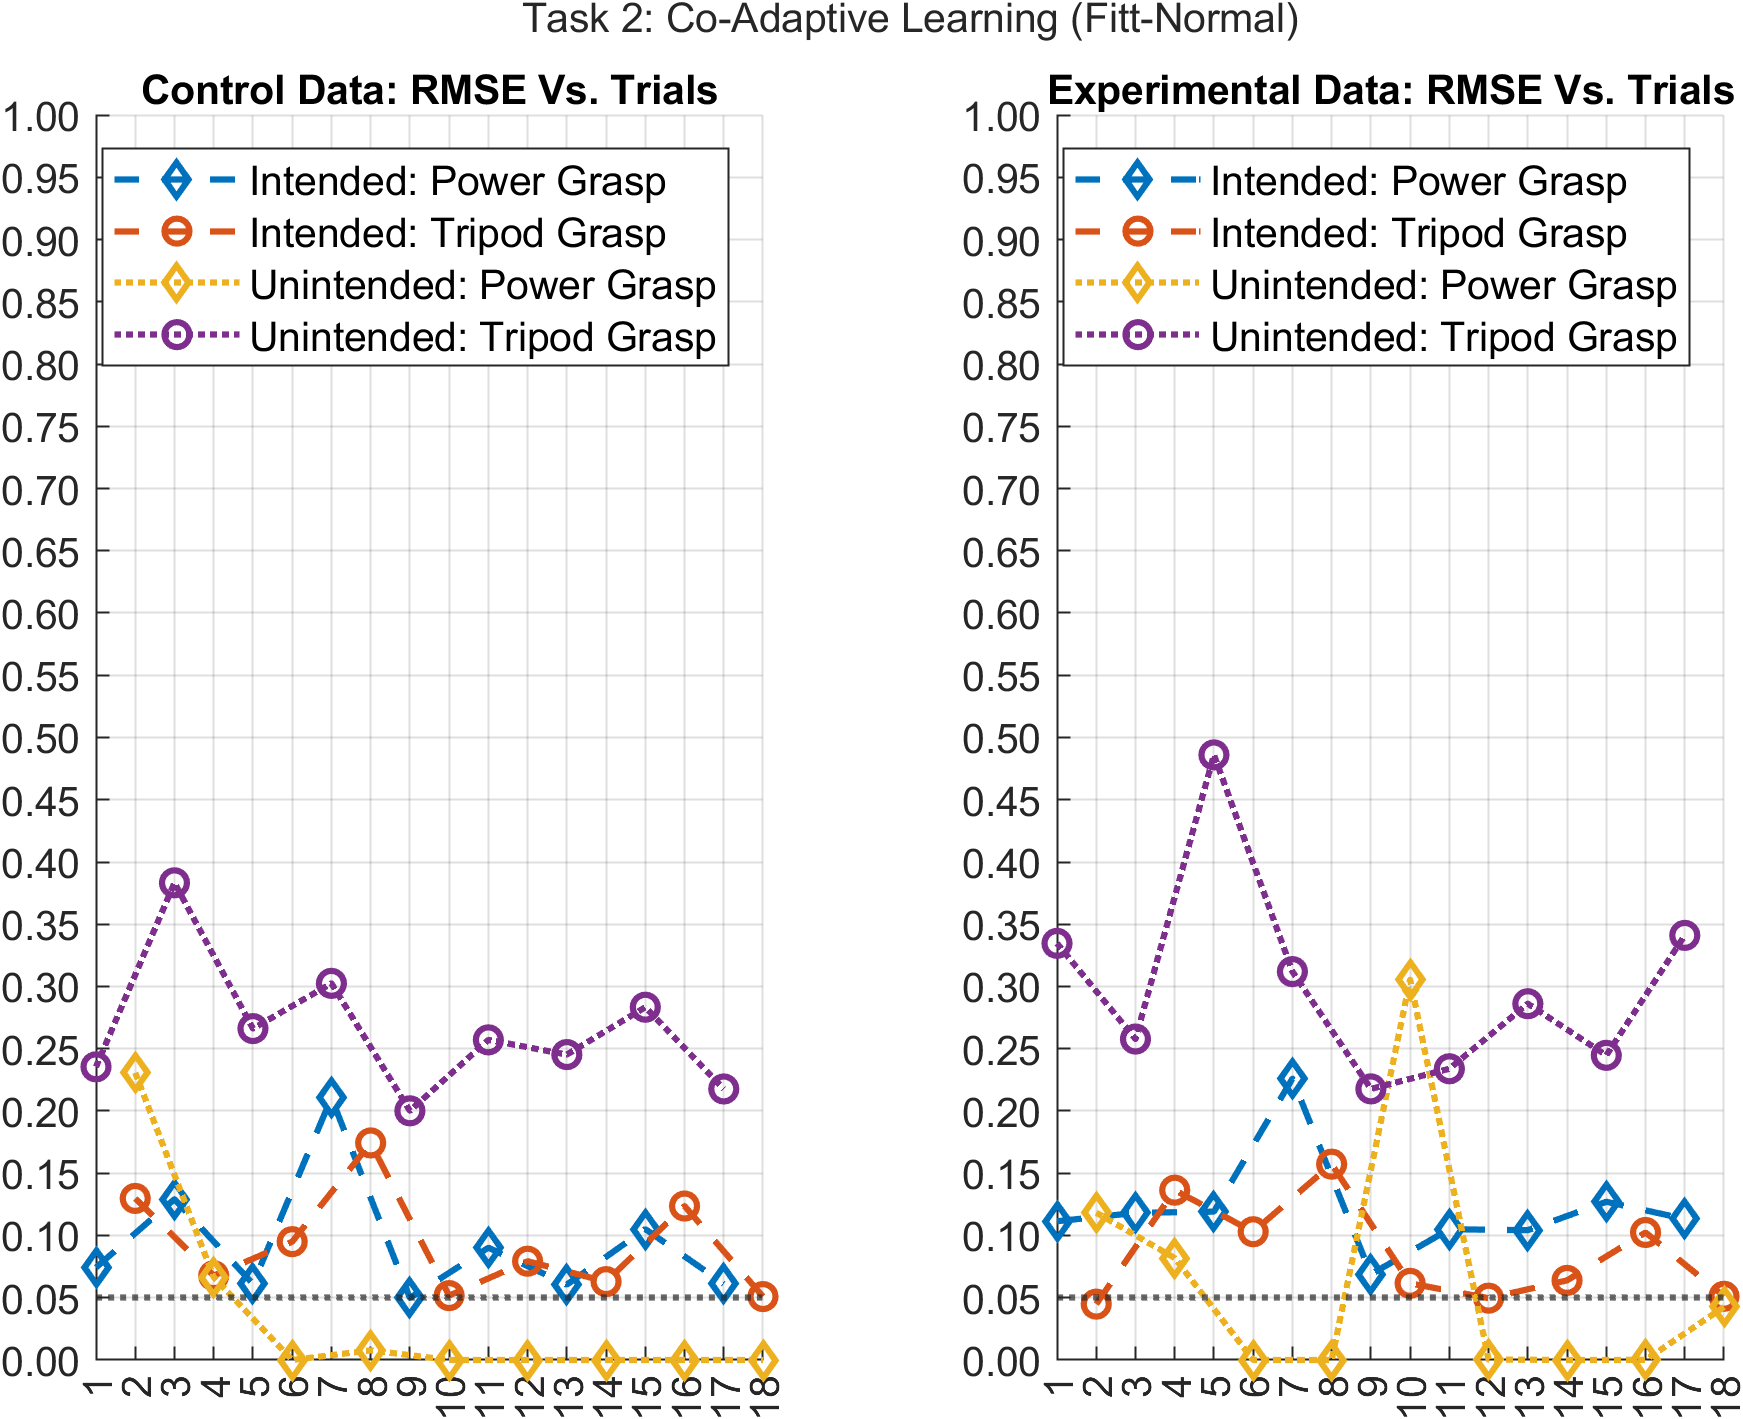
\includegraphics[width = \figWidth]{t2-rmse-fnorm.png}
\end{figure}
\begin{figure}
    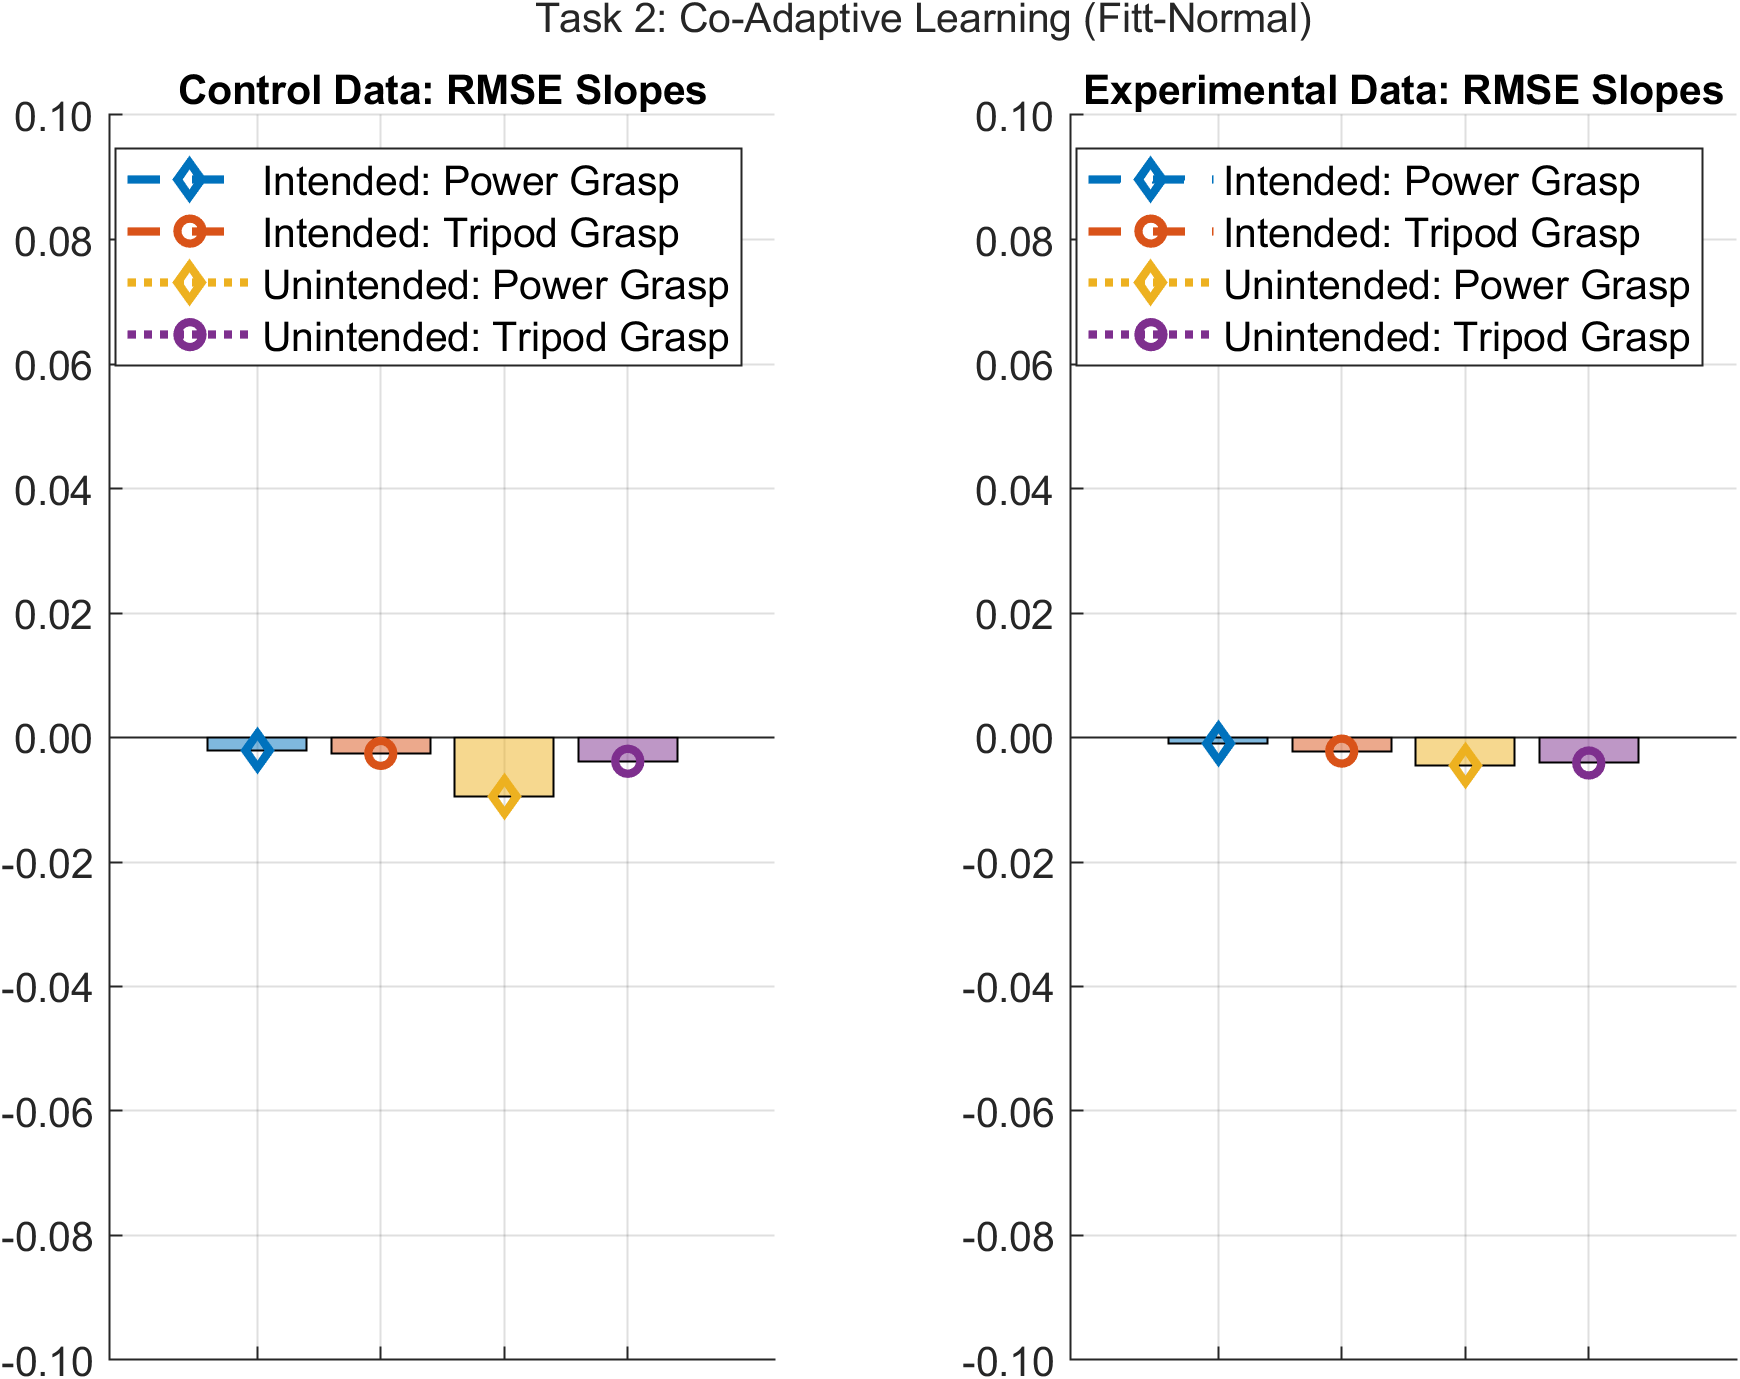
\includegraphics[width = \figWidth]{t2-bar-fnorm.png}
\end{figure}
\begin{figure}
    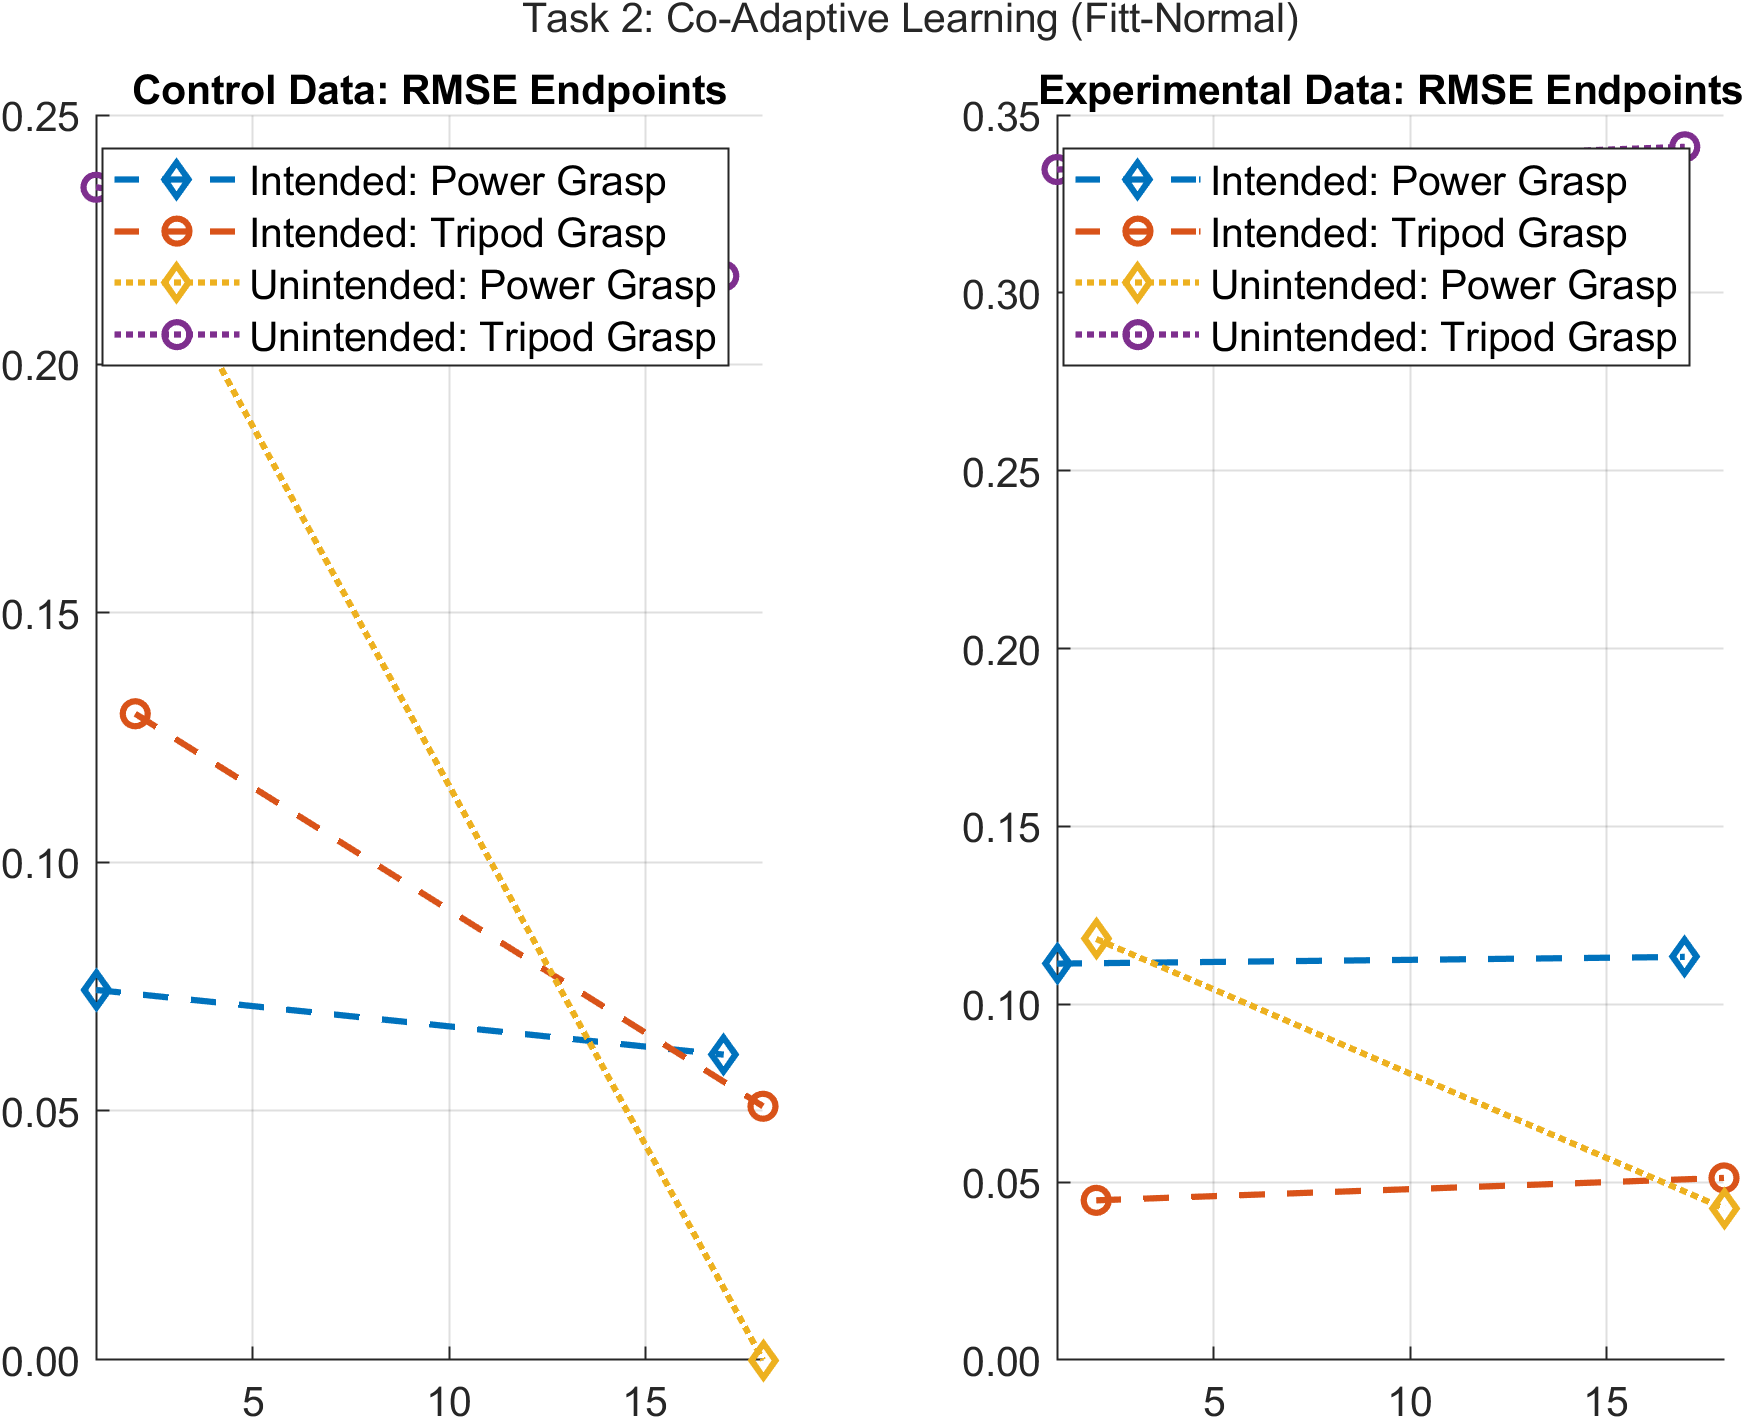
\includegraphics[width = \figWidth]{t2-spaghetti-fnorm.png}
\end{figure}
%%%%%%%
\begin{landscape}
    \begin{figure}
        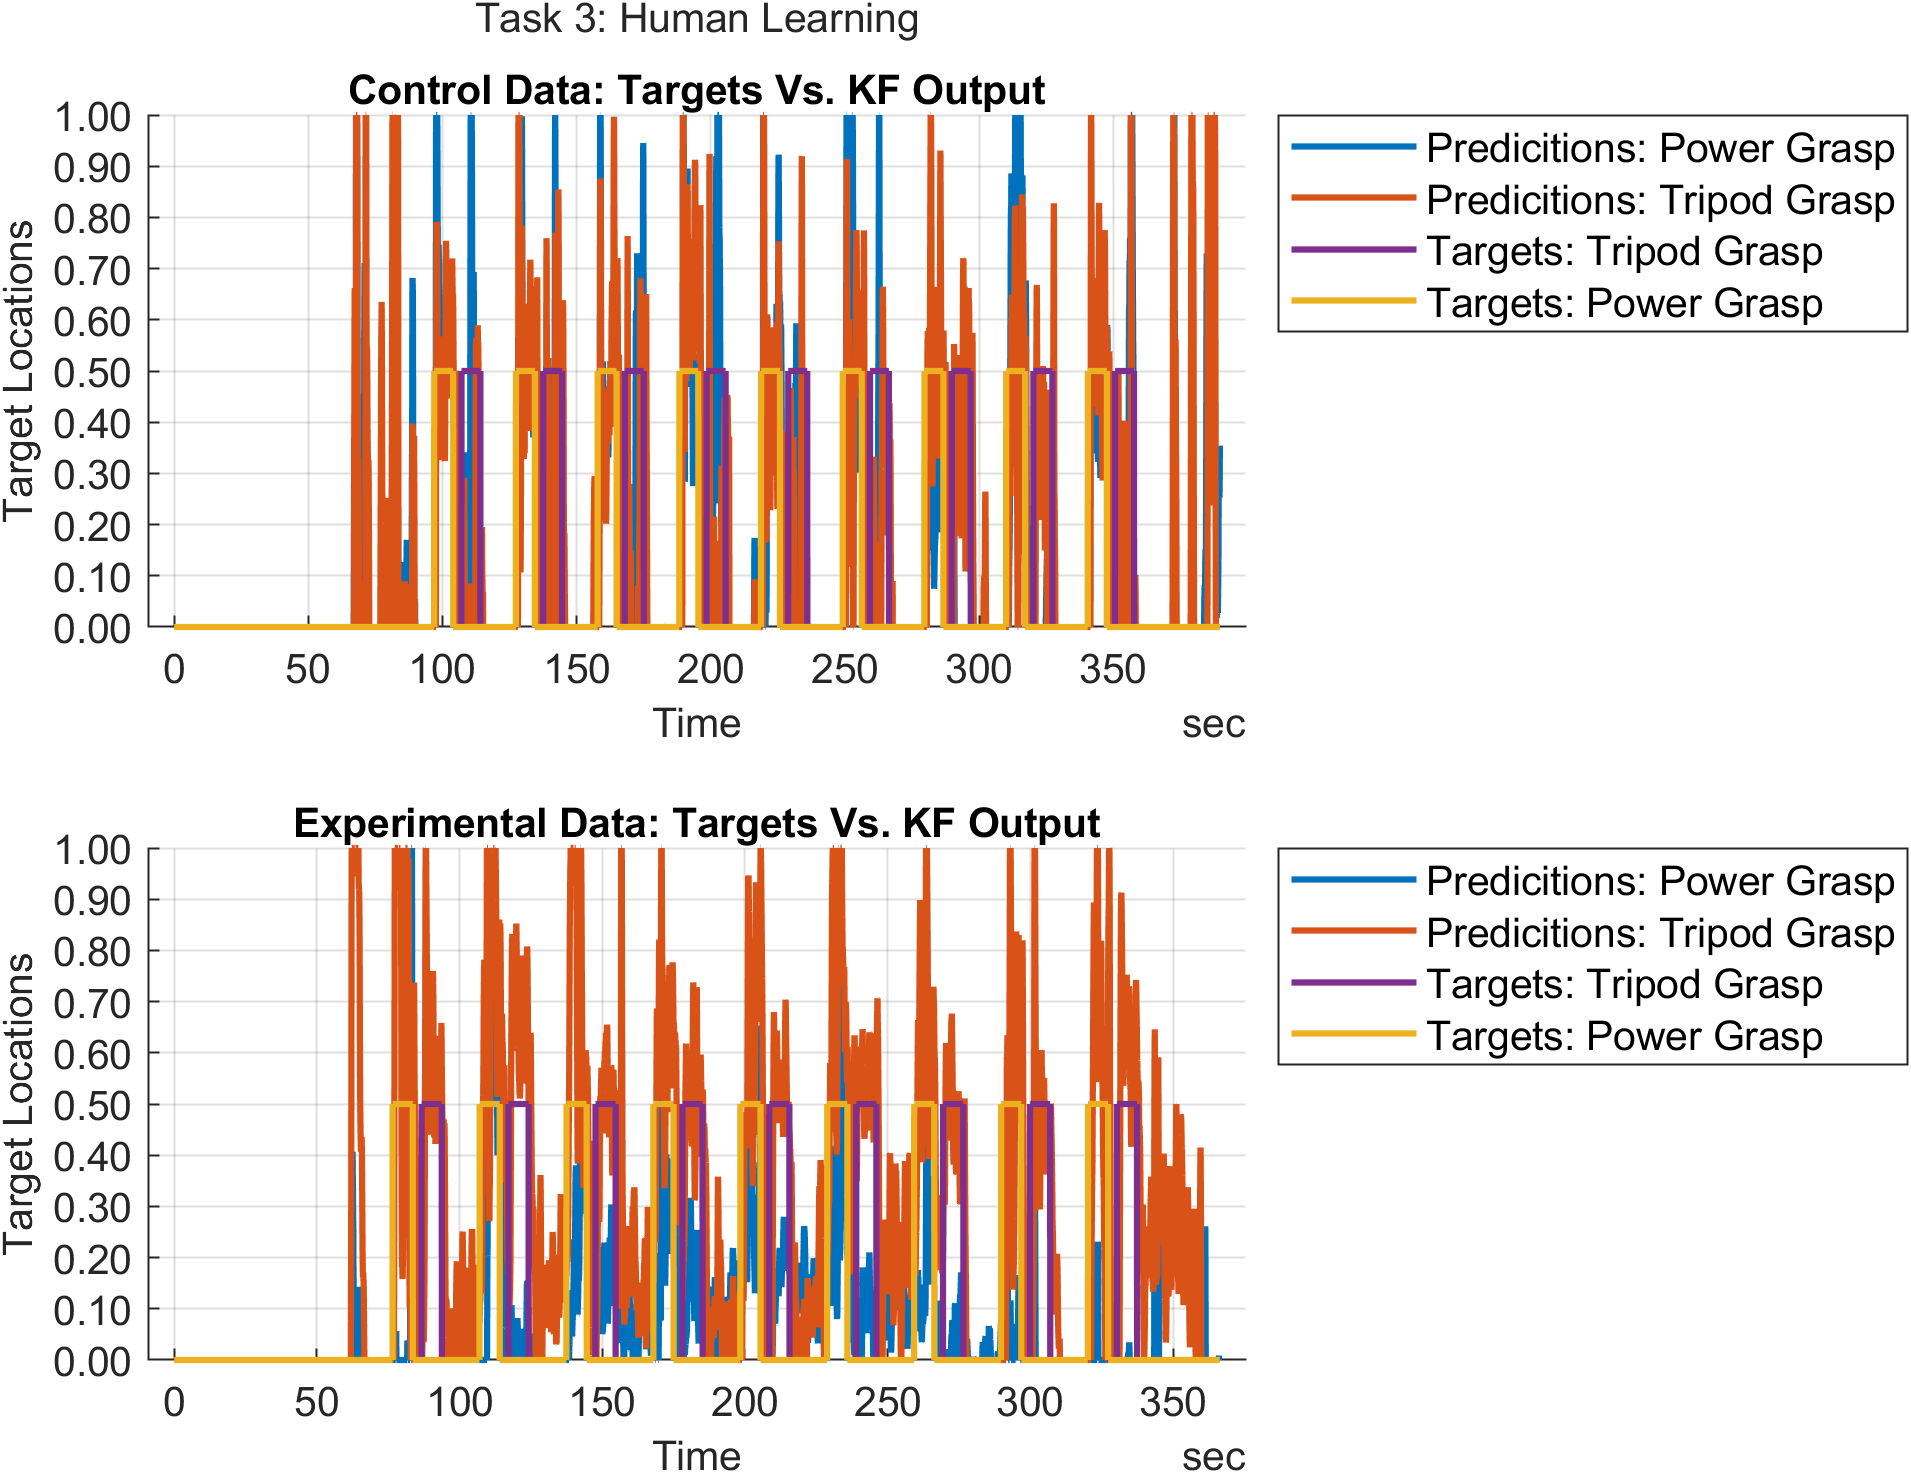
\includegraphics[width = \figWidthLarge]{t3-kf-out.png}
    \end{figure}
\end{landscape}
\begin{figure}
    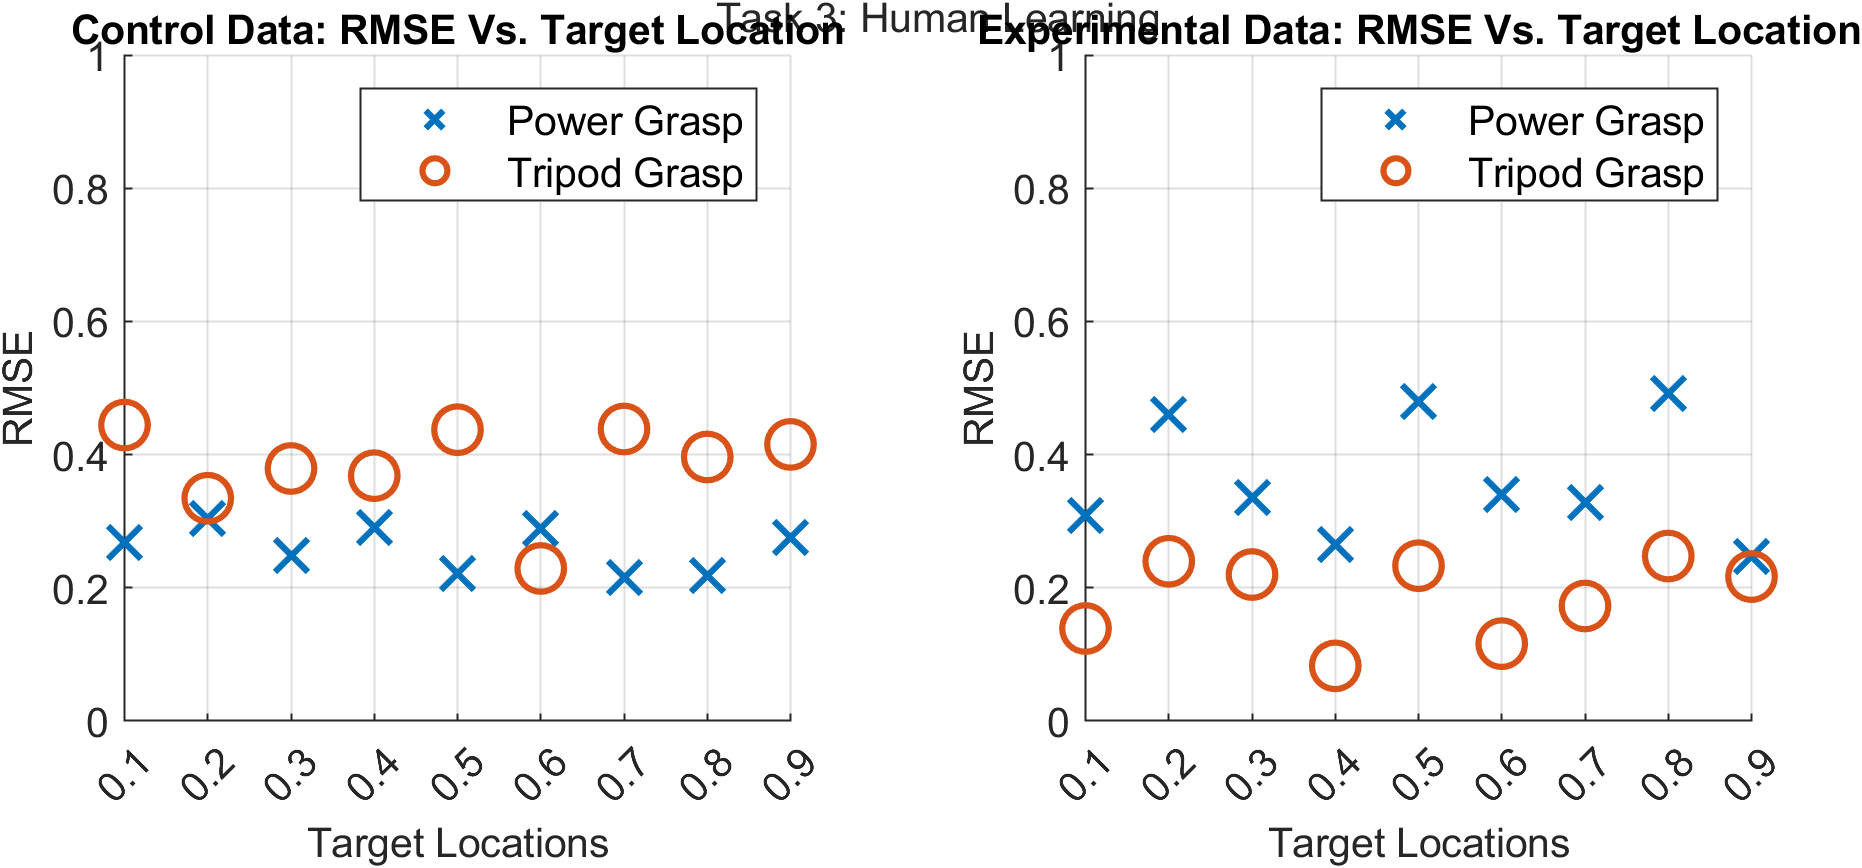
\includegraphics[width = \figWidth]{t3-rmse-reg.png}
\end{figure}
\newpage
\clearpage
\begin{figure}
    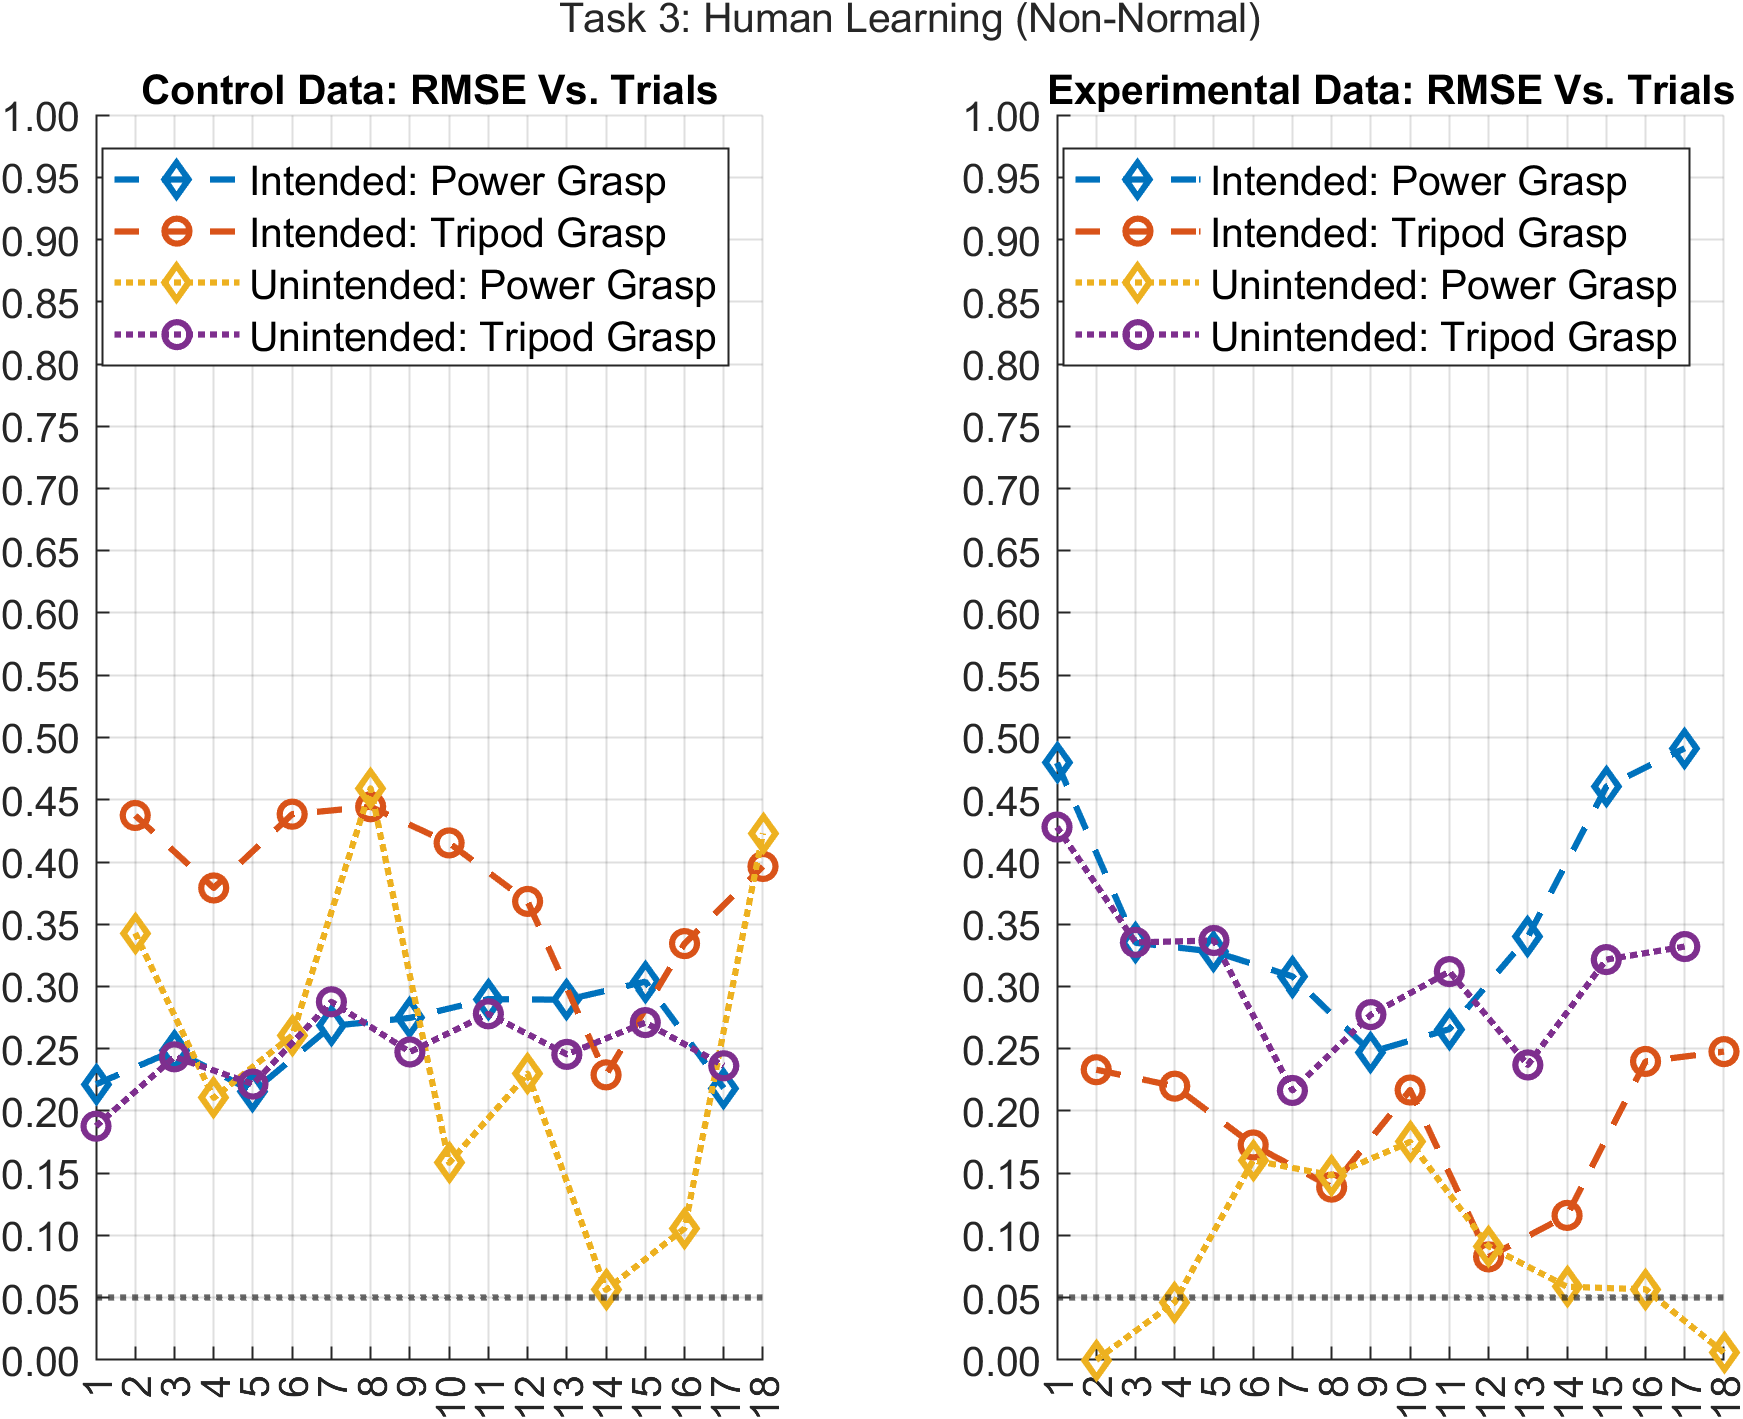
\includegraphics[width = \figWidth]{t3-rmse-xnorm.png}
\end{figure}
\begin{figure}
    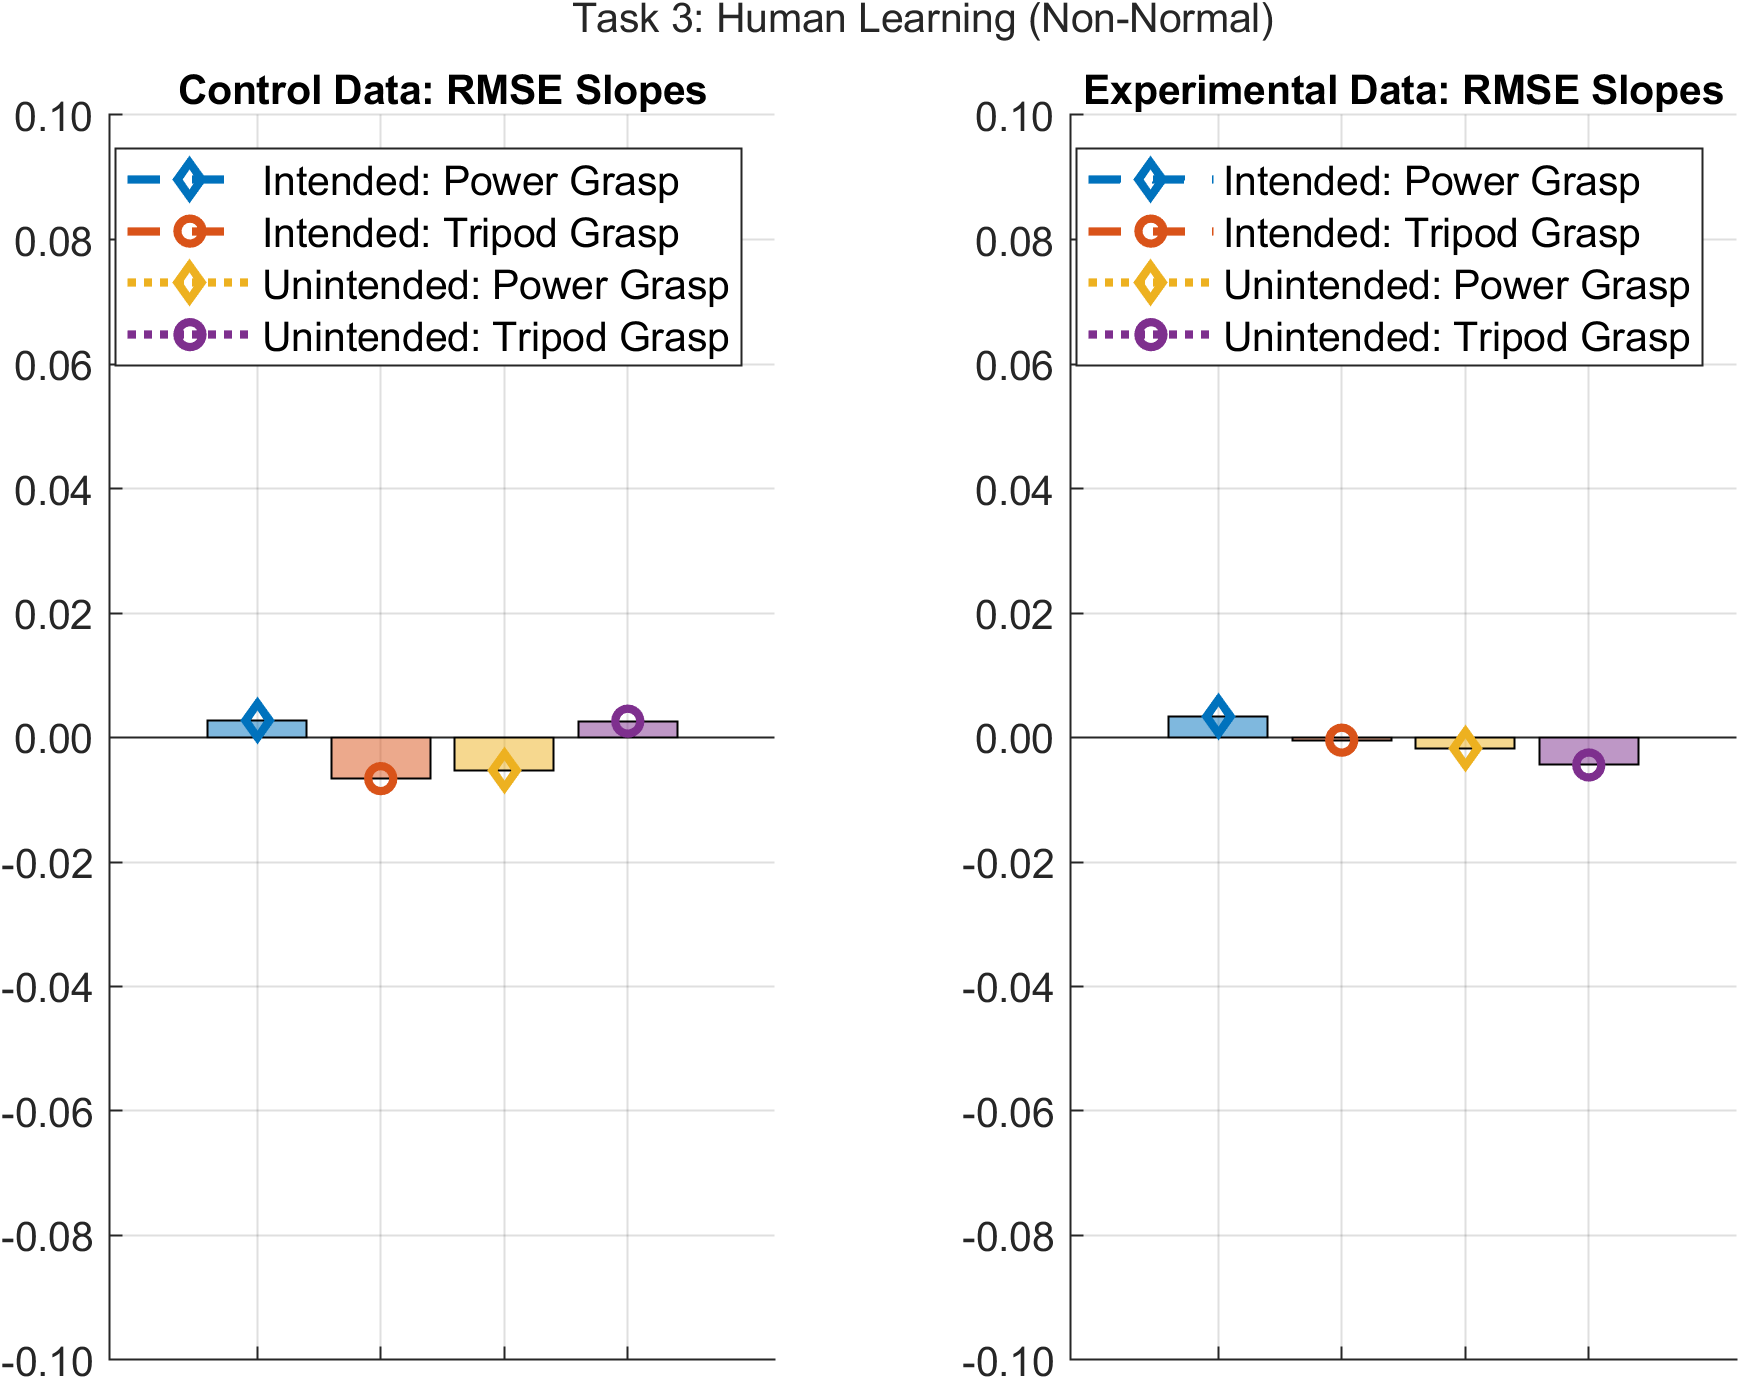
\includegraphics[width = \figWidth]{t3-bar-xnorm.png}
\end{figure}
\begin{figure}
    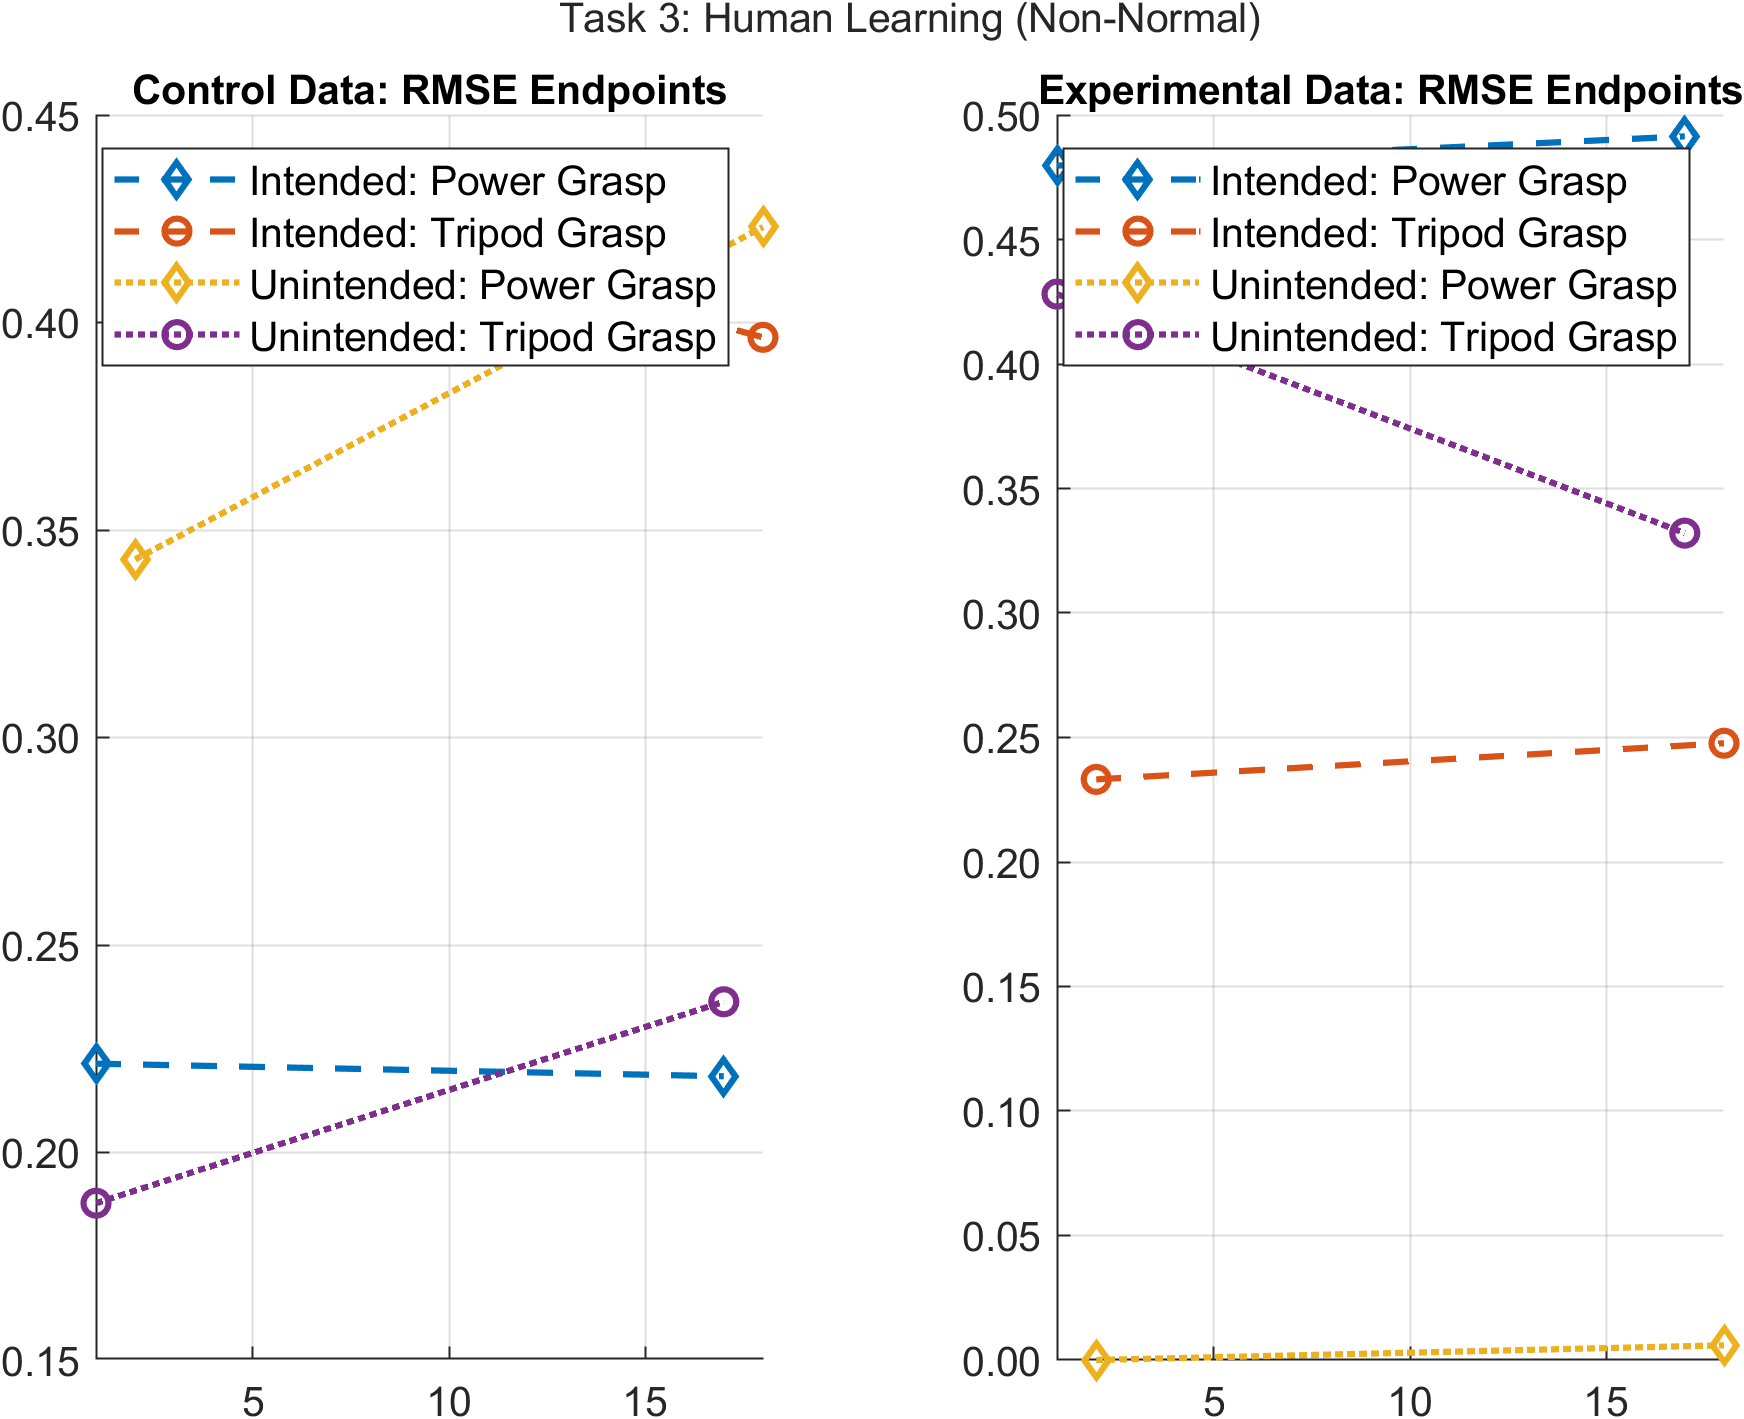
\includegraphics[width = \figWidth]{t3-spaghetti-xnorm.png}
\end{figure}

\begin{figure}
    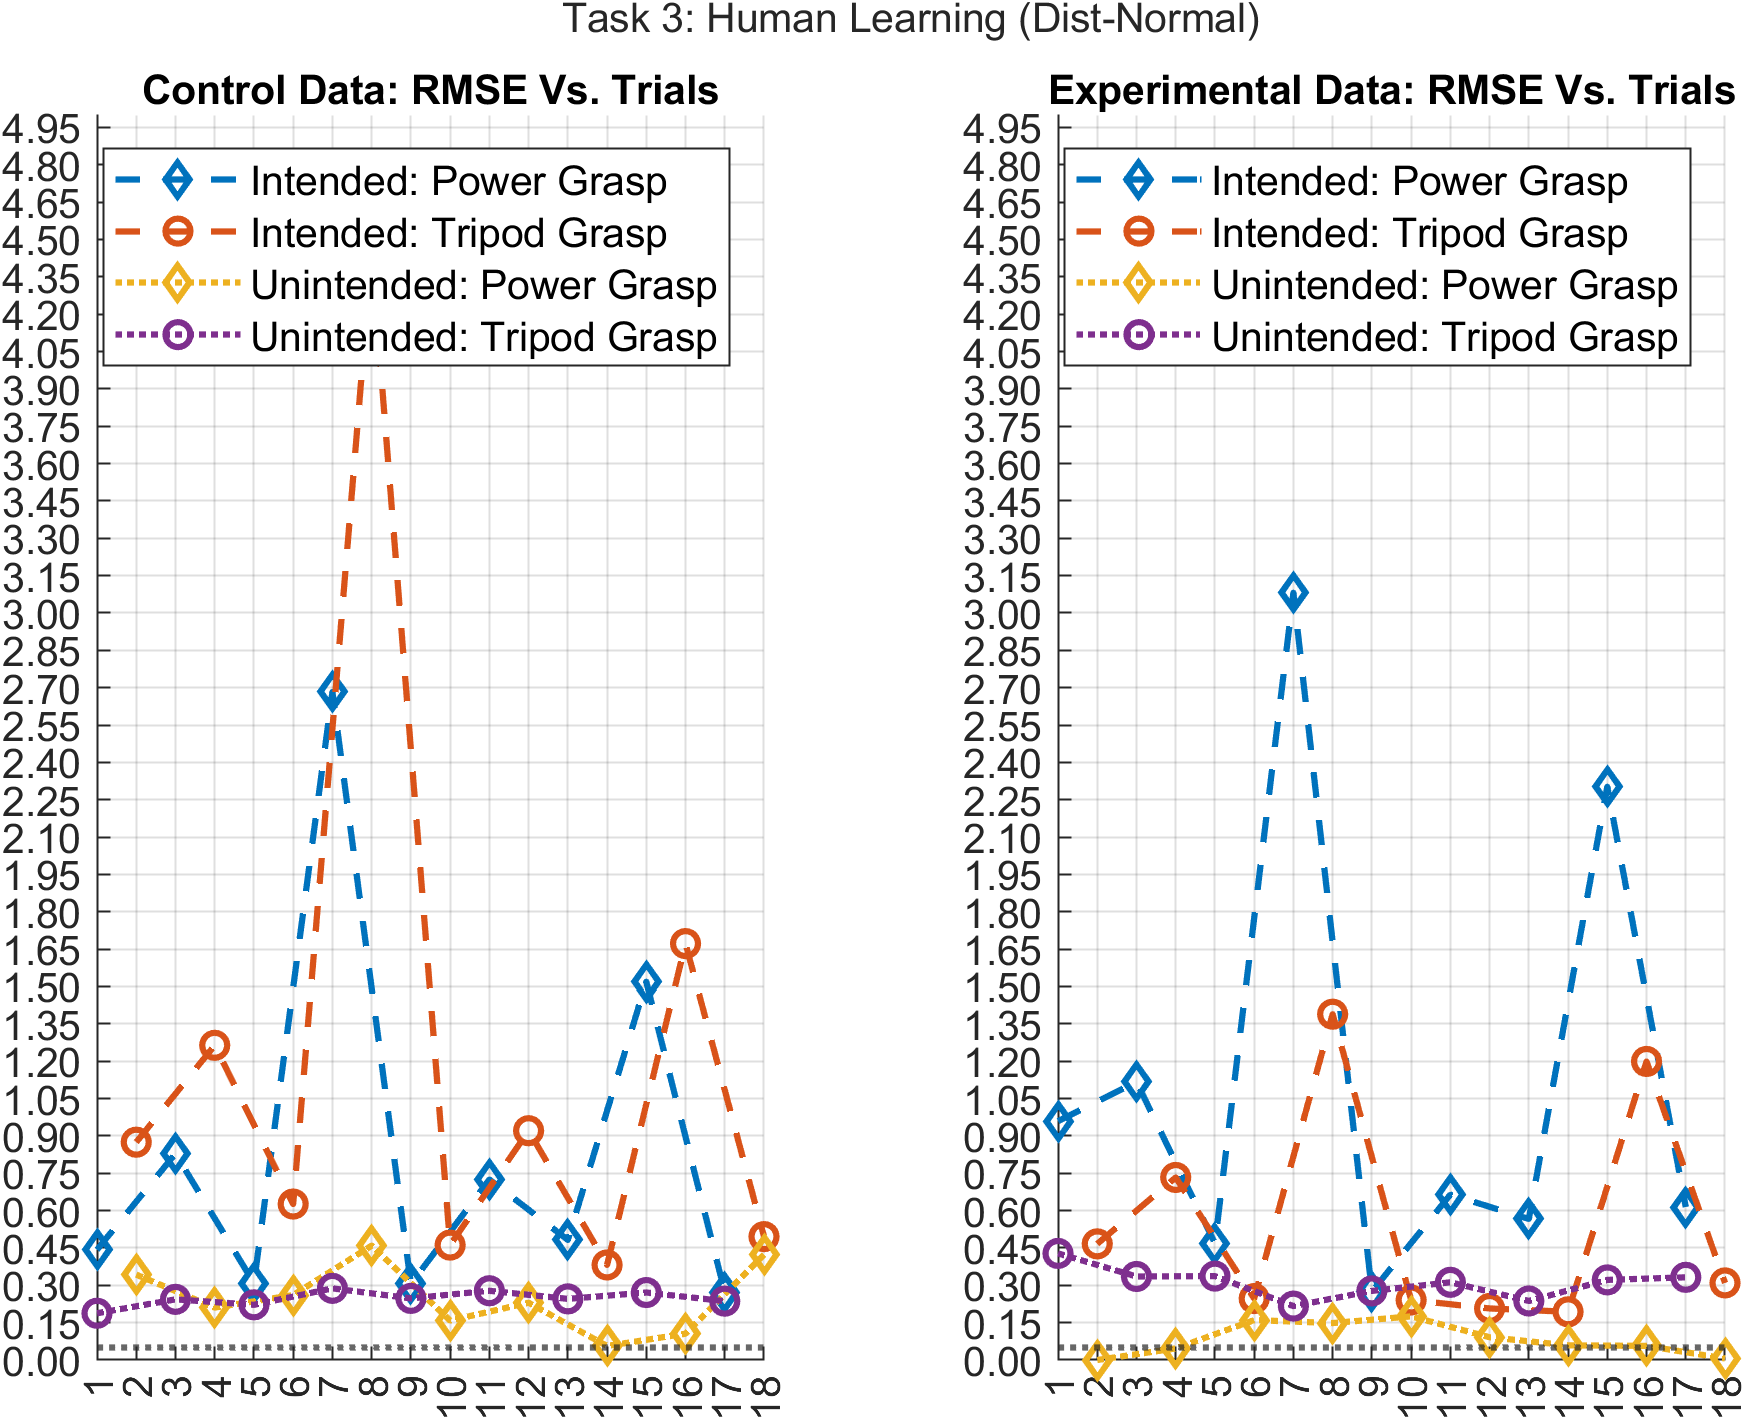
\includegraphics[width = \figWidth]{t3-rmse-dnorm.png}
\end{figure}
\begin{figure}
    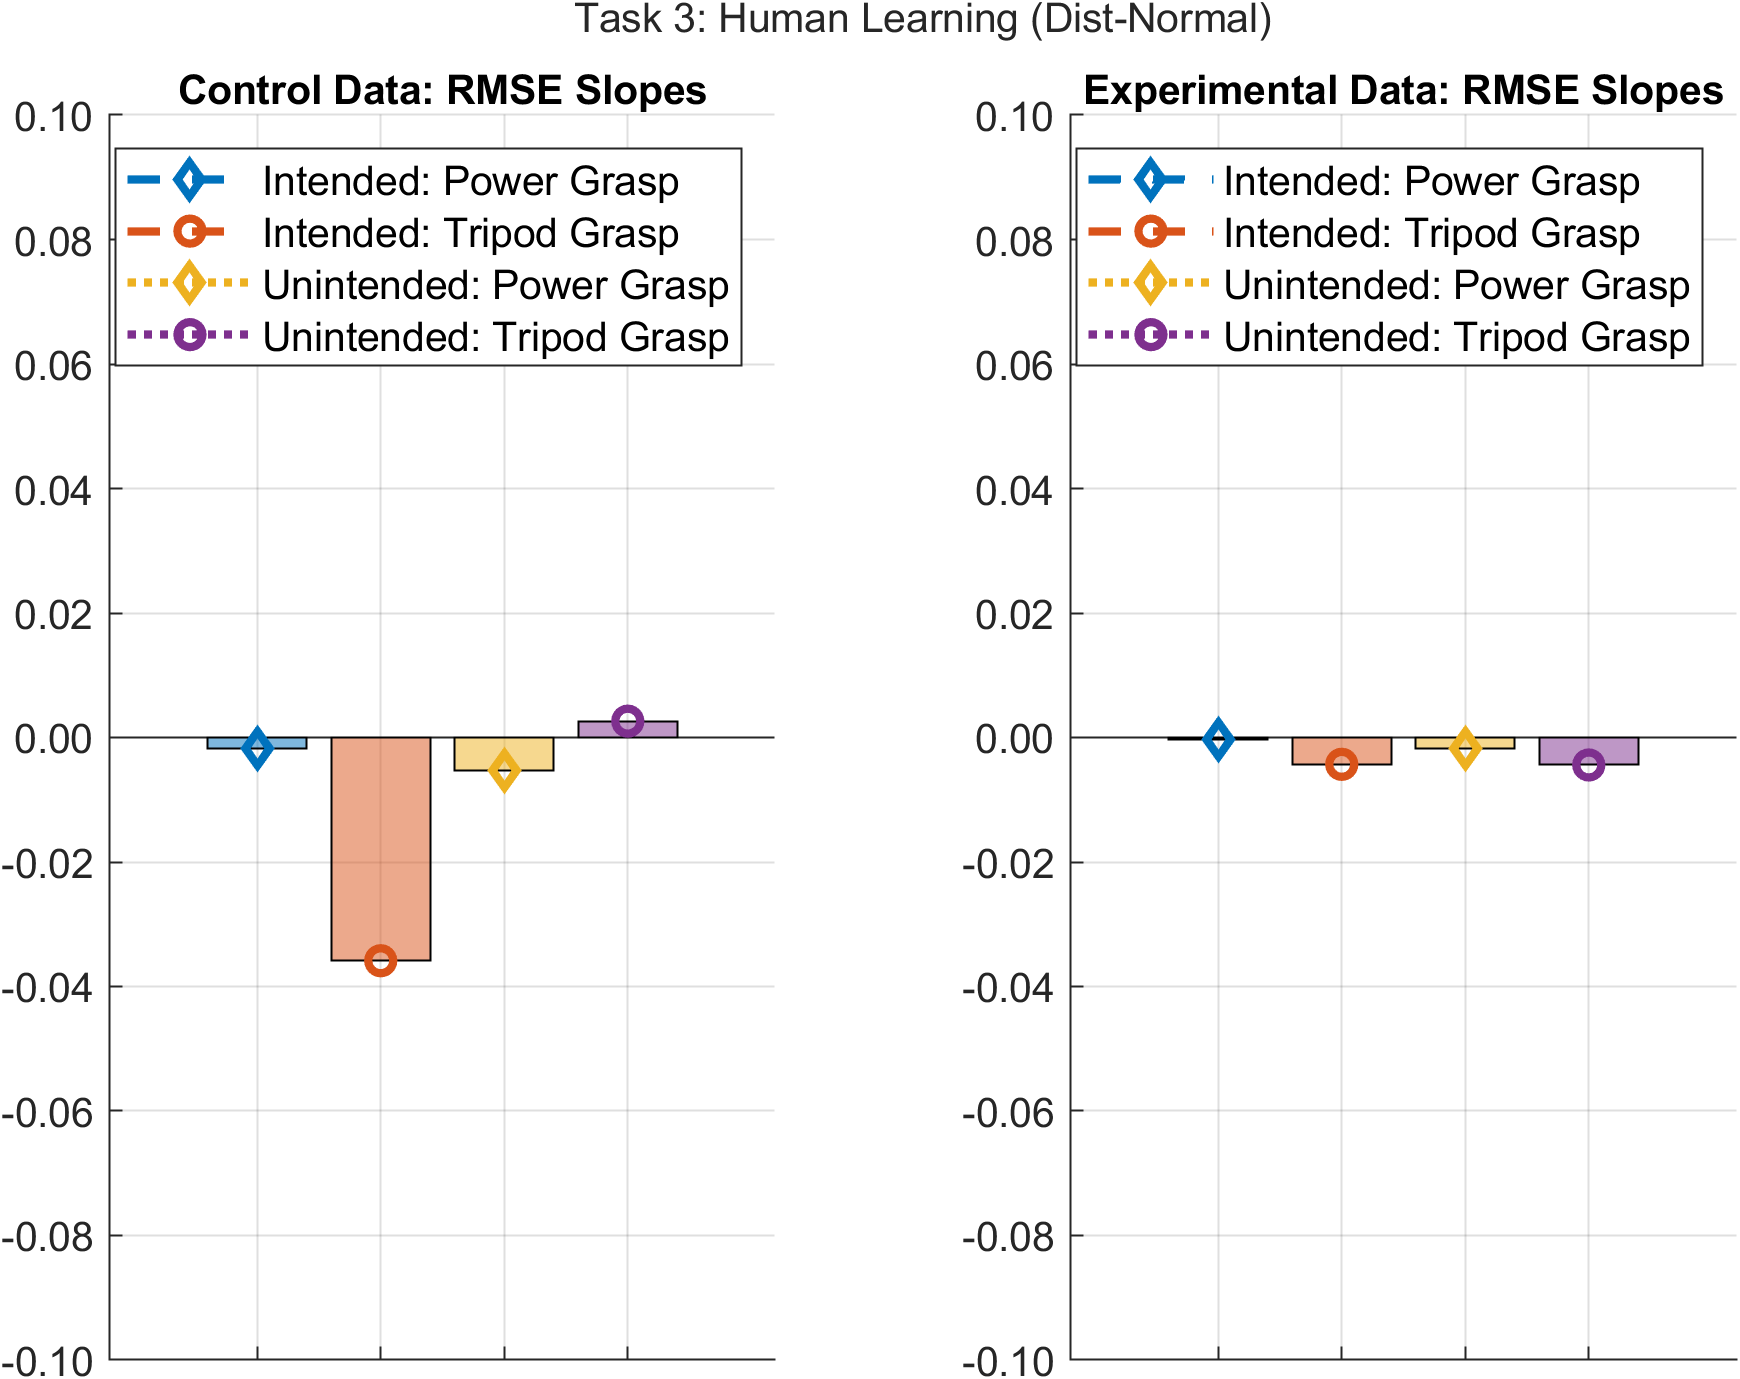
\includegraphics[width = \figWidth]{t3-bar-dnorm.png}
\end{figure}
\begin{figure}
    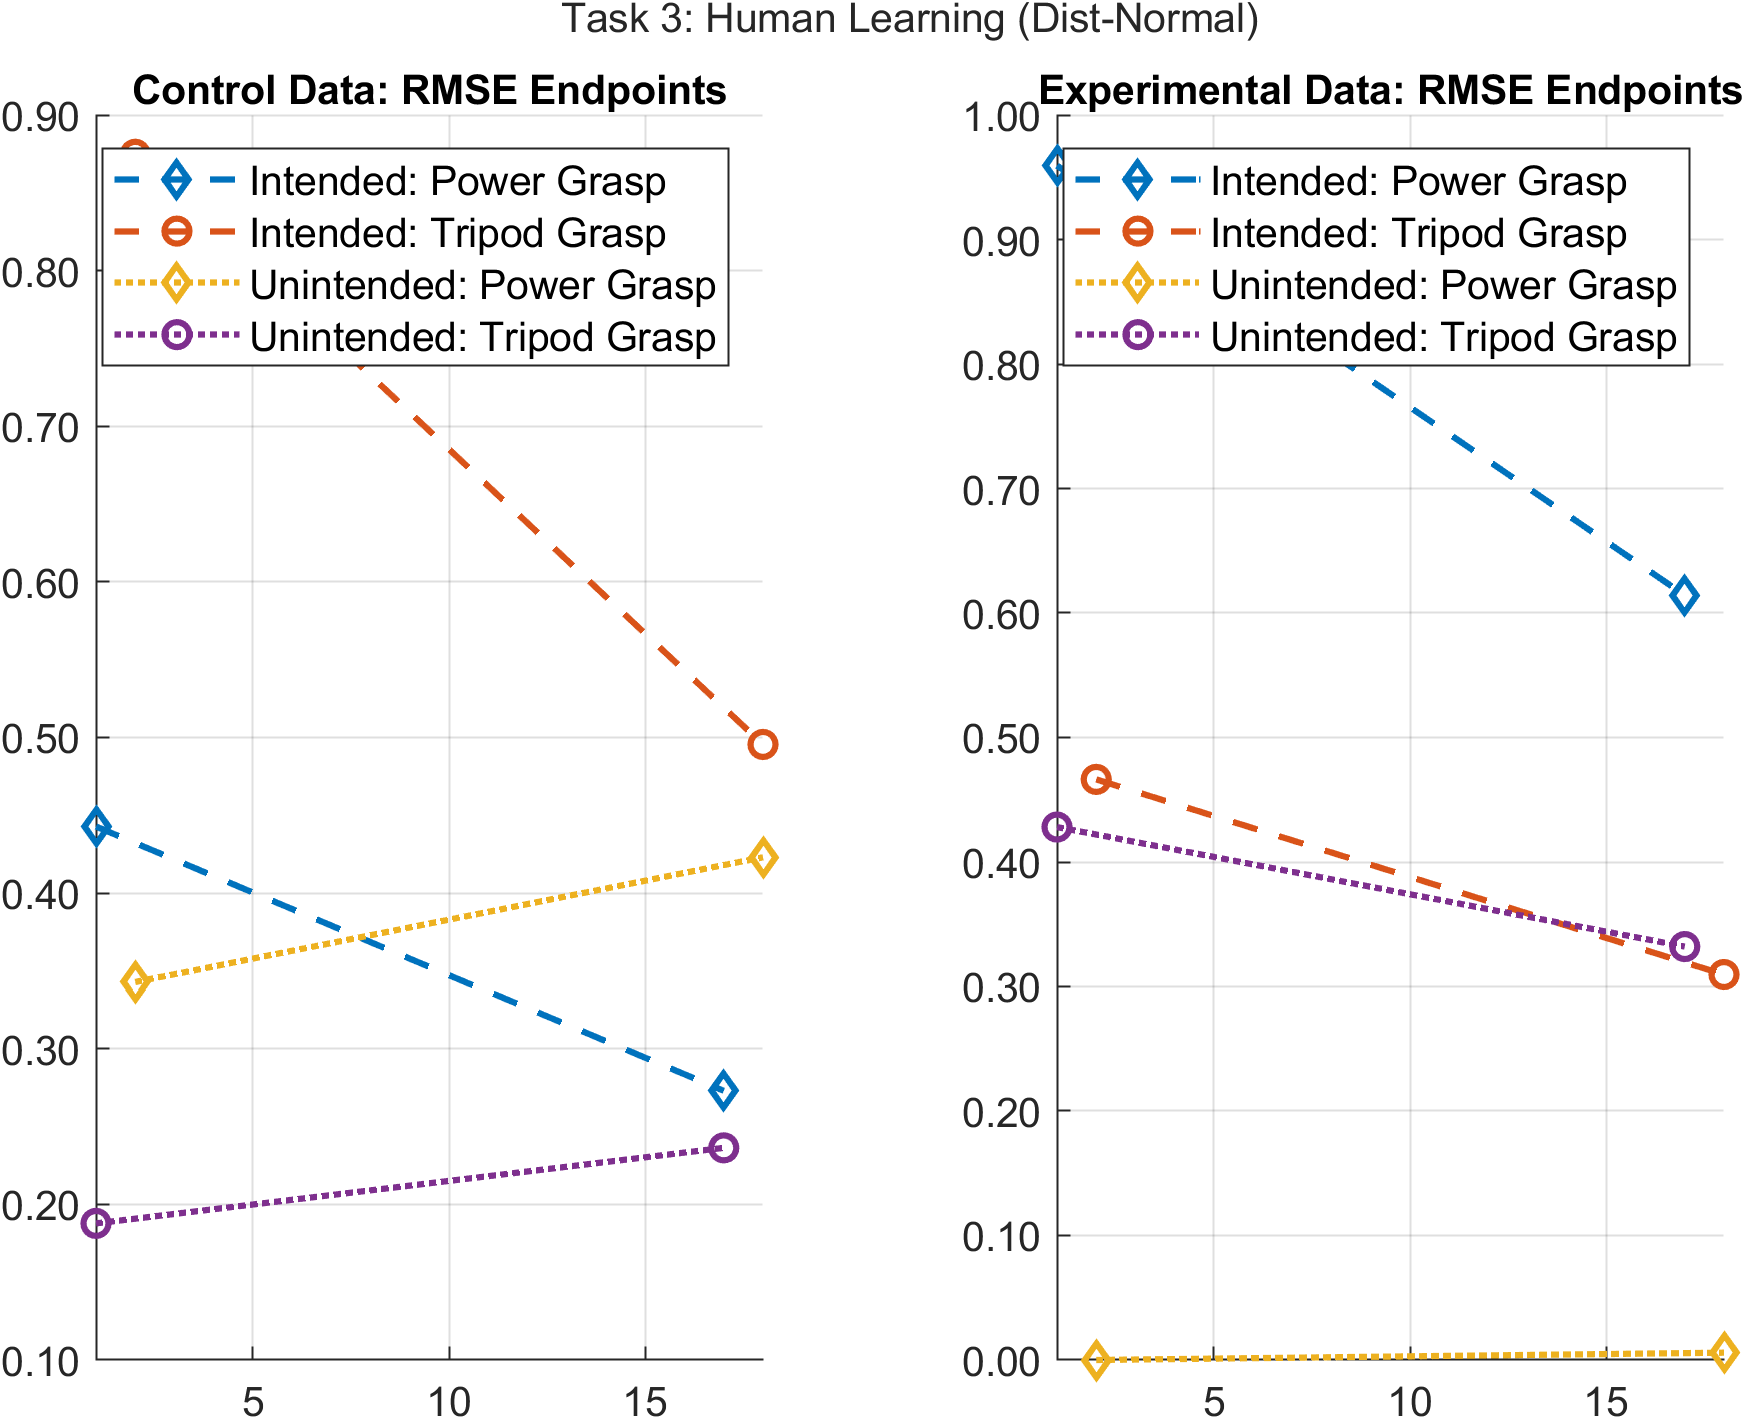
\includegraphics[width = \figWidth]{t3-spaghetti-dnorm.png}
\end{figure}

\begin{figure}
    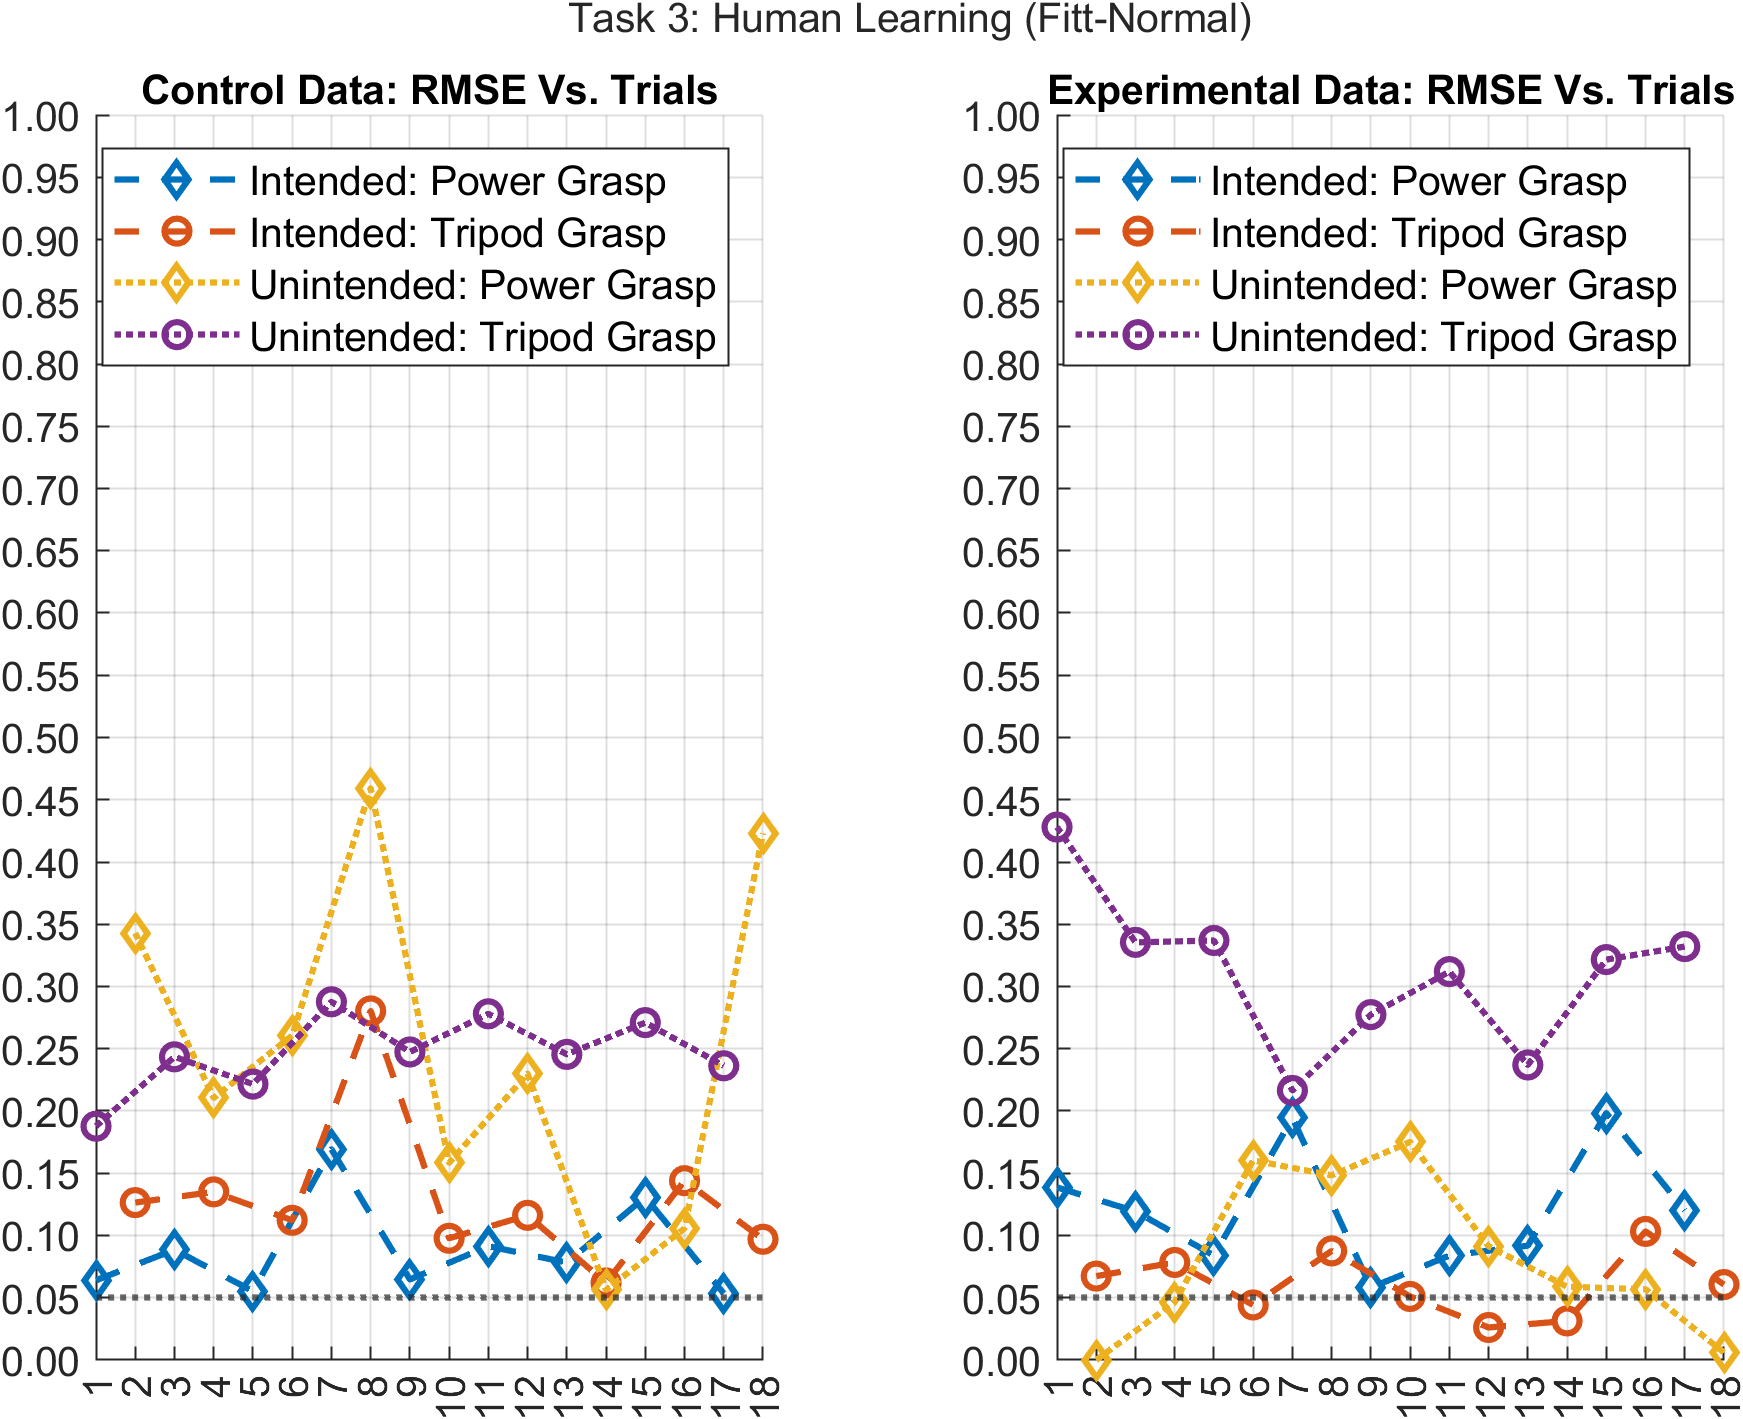
\includegraphics[width = \figWidth]{t3-rmse-fnorm.png}
\end{figure}
\begin{figure}
    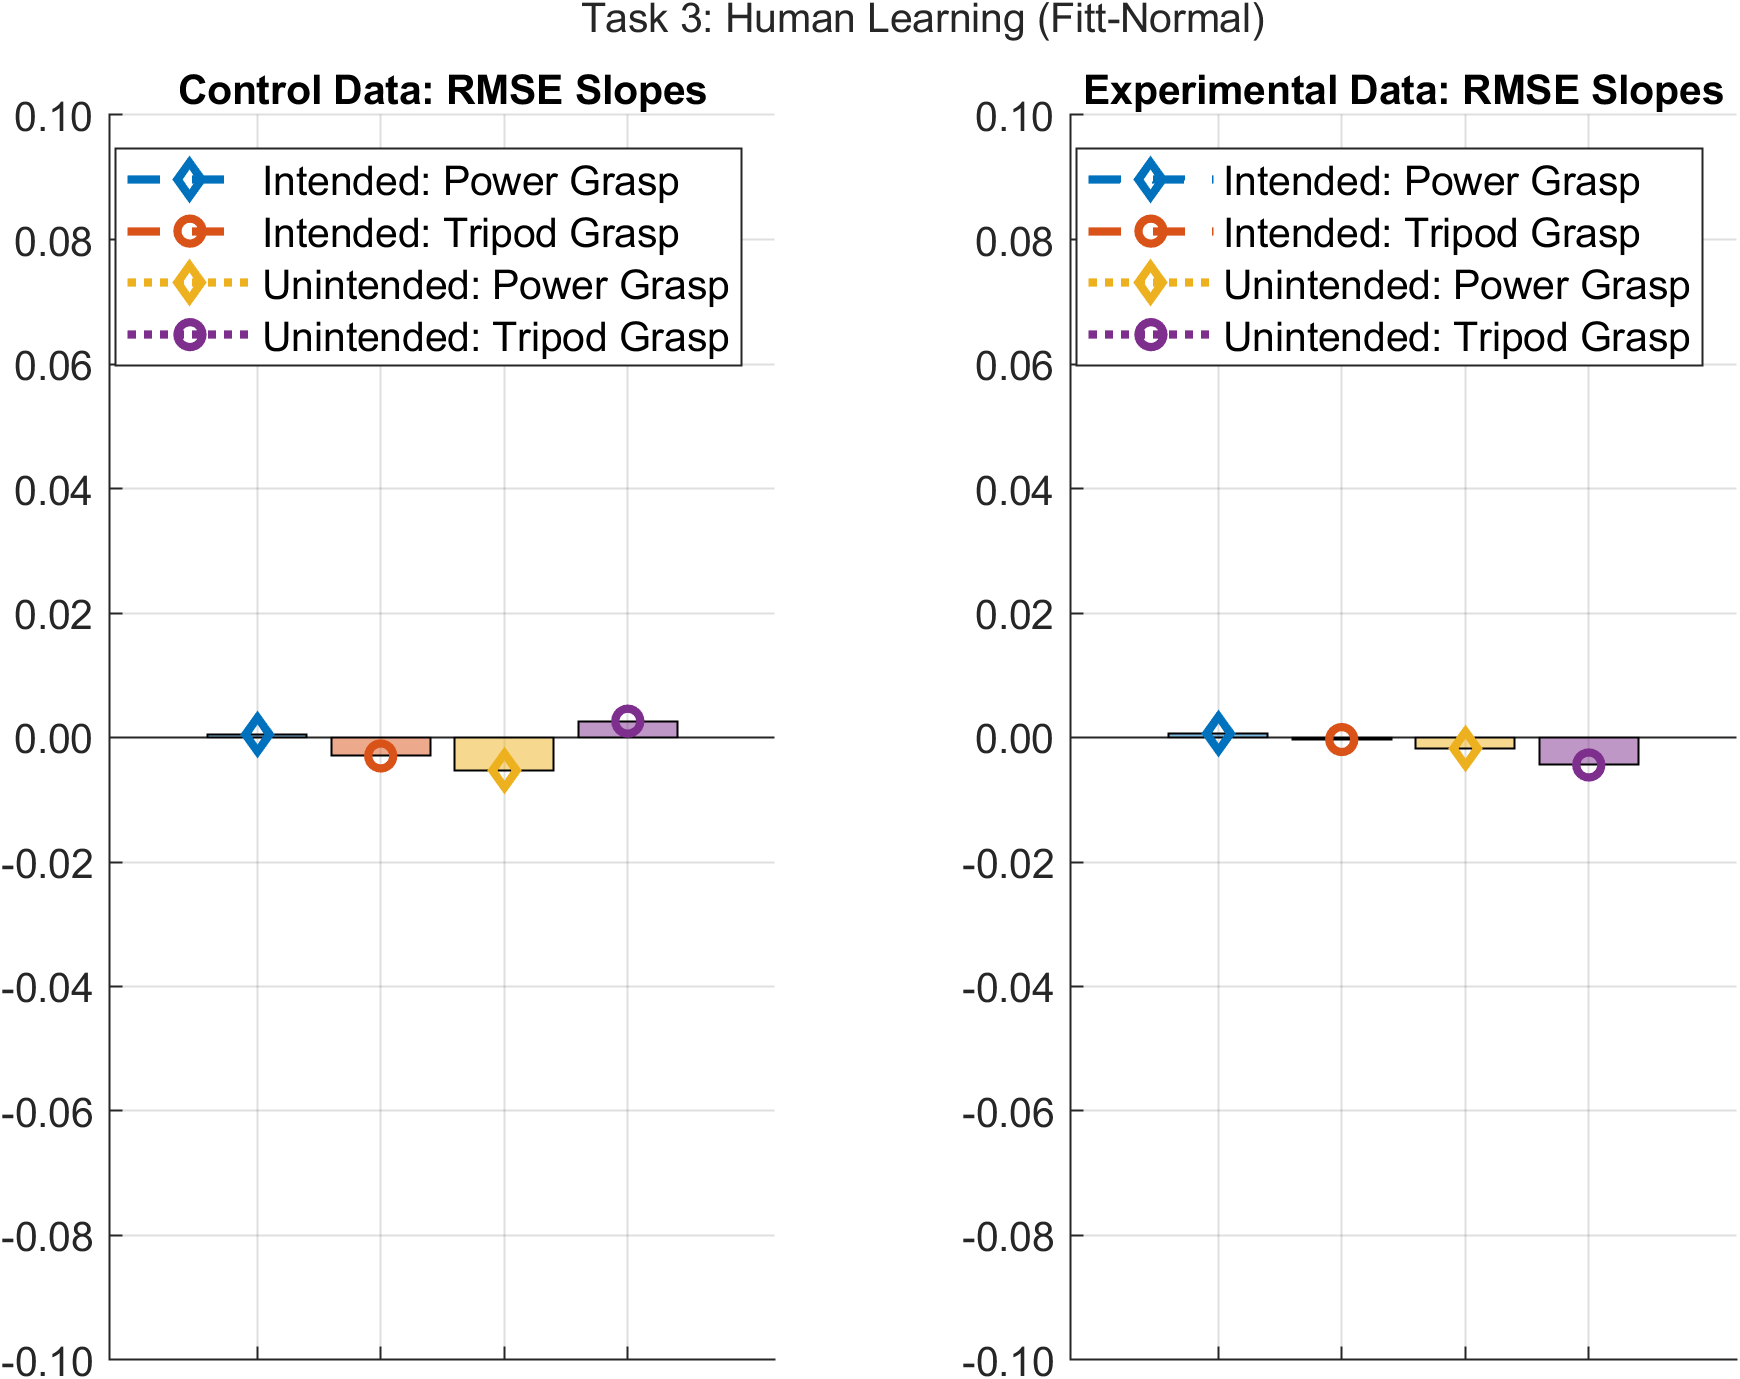
\includegraphics[width = \figWidth]{t3-bar-fnorm.png}
\end{figure}
\begin{figure}
    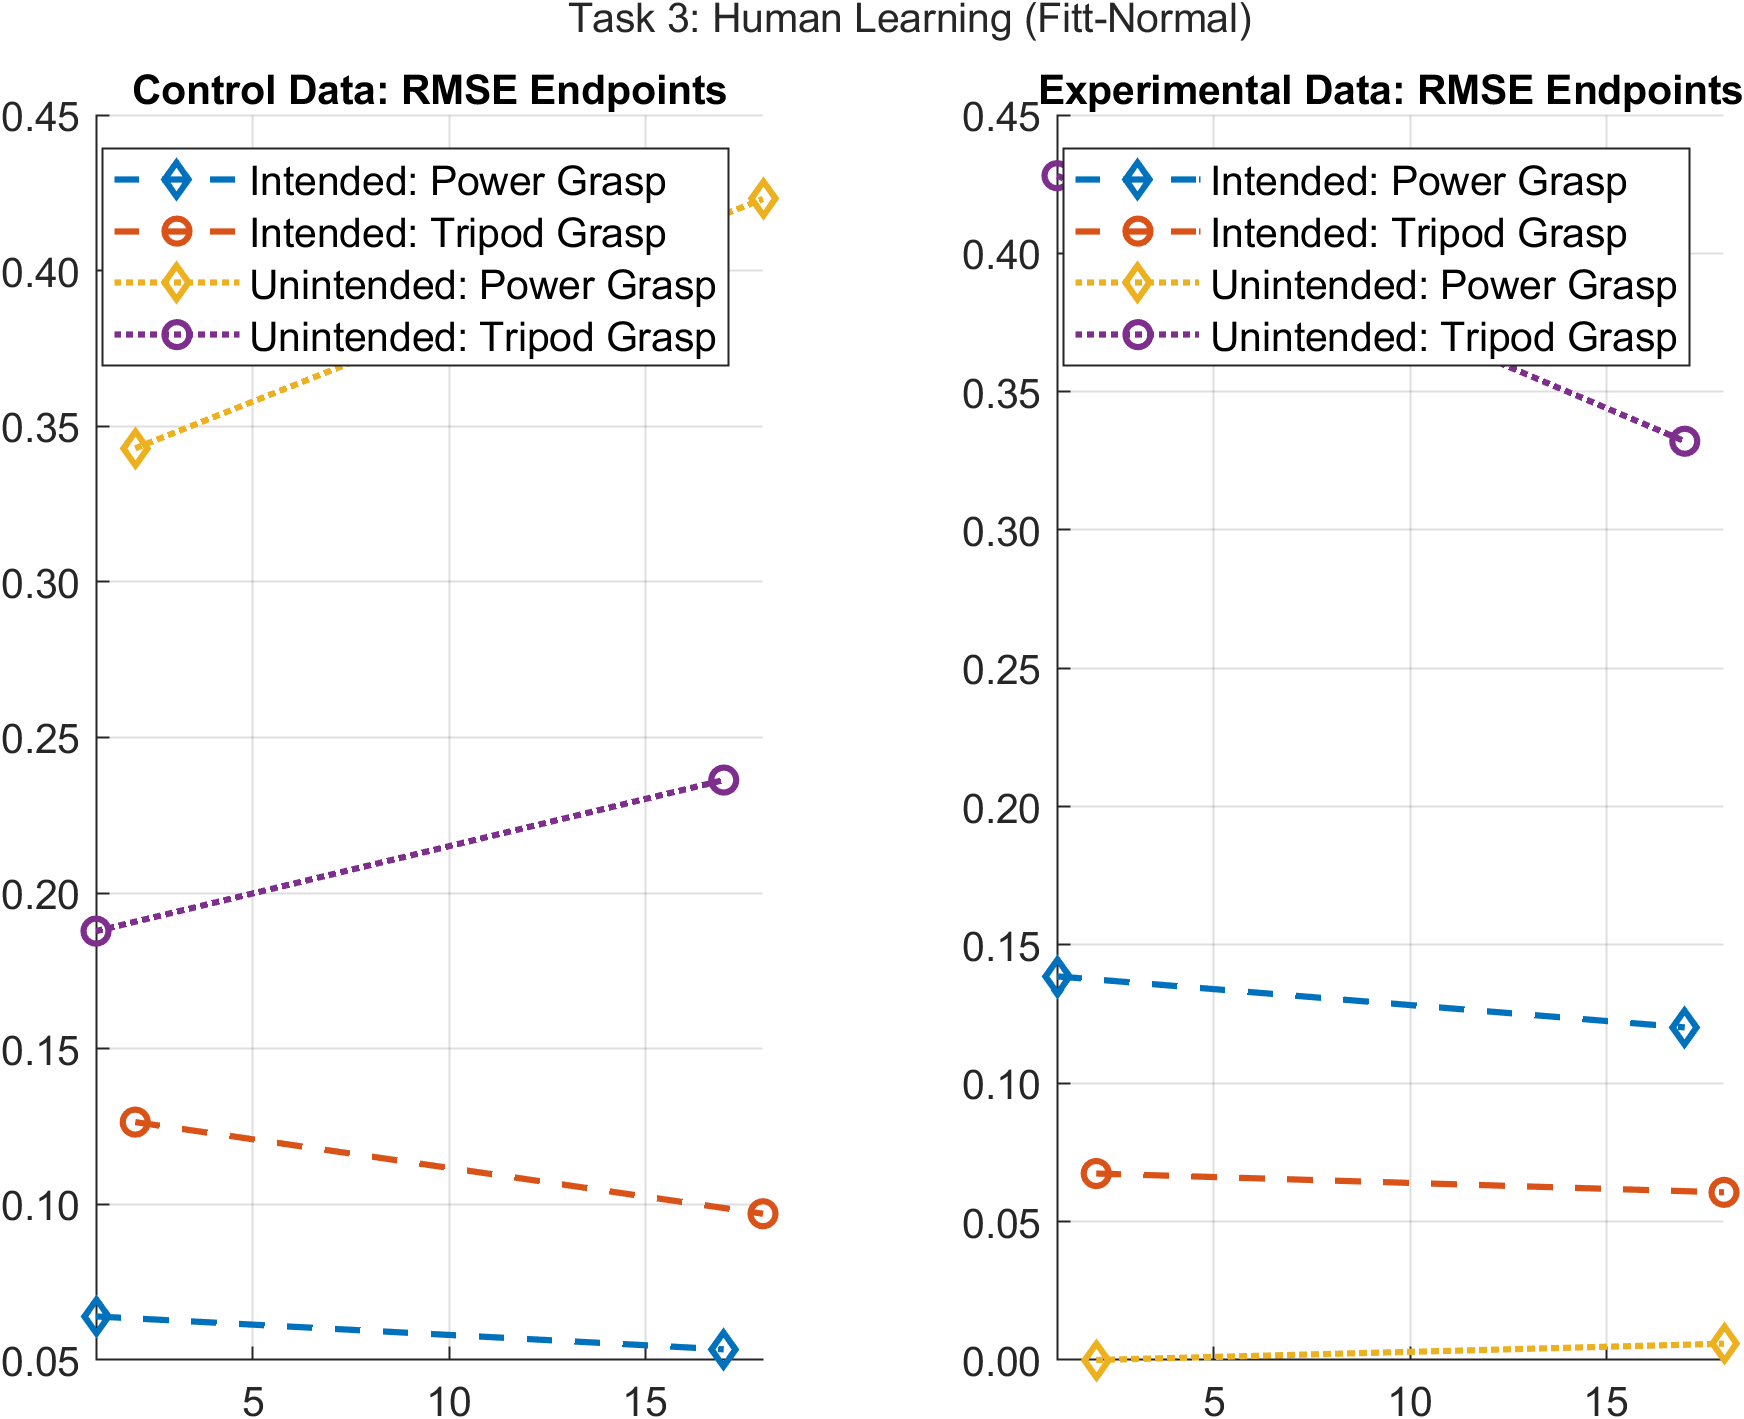
\includegraphics[width = \figWidth]{t3-spaghetti-fnorm.png}
\end{figure}
\end{document}